% Options for packages loaded elsewhere
\PassOptionsToPackage{unicode}{hyperref}
\PassOptionsToPackage{hyphens}{url}
%
\documentclass[
  11pt,
  a4paper,
]{scrbook}

\usepackage{amsmath,amssymb}
\usepackage{setspace}
\usepackage{iftex}
\ifPDFTeX
  \usepackage[T1]{fontenc}
  \usepackage[utf8]{inputenc}
  \usepackage{textcomp} % provide euro and other symbols
\else % if luatex or xetex
  \usepackage{unicode-math}
  \defaultfontfeatures{Scale=MatchLowercase}
  \defaultfontfeatures[\rmfamily]{Ligatures=TeX,Scale=1}
\fi
\usepackage{lmodern}
\ifPDFTeX\else  
    % xetex/luatex font selection
\fi
% Use upquote if available, for straight quotes in verbatim environments
\IfFileExists{upquote.sty}{\usepackage{upquote}}{}
\IfFileExists{microtype.sty}{% use microtype if available
  \usepackage[]{microtype}
  \UseMicrotypeSet[protrusion]{basicmath} % disable protrusion for tt fonts
}{}
\makeatletter
\@ifundefined{KOMAClassName}{% if non-KOMA class
  \IfFileExists{parskip.sty}{%
    \usepackage{parskip}
  }{% else
    \setlength{\parindent}{0pt}
    \setlength{\parskip}{6pt plus 2pt minus 1pt}}
}{% if KOMA class
  \KOMAoptions{parskip=half}}
\makeatother
\usepackage{xcolor}
\usepackage[textheight=9in,,textwidth=6.5in,,top=1in,,headheight=14pt,,headsep=25pt,,footskip=30pt]{geometry}
\setlength{\emergencystretch}{3em} % prevent overfull lines
\setcounter{secnumdepth}{2}
% Make \paragraph and \subparagraph free-standing
\makeatletter
\ifx\paragraph\undefined\else
  \let\oldparagraph\paragraph
  \renewcommand{\paragraph}{
    \@ifstar
      \xxxParagraphStar
      \xxxParagraphNoStar
  }
  \newcommand{\xxxParagraphStar}[1]{\oldparagraph*{#1}\mbox{}}
  \newcommand{\xxxParagraphNoStar}[1]{\oldparagraph{#1}\mbox{}}
\fi
\ifx\subparagraph\undefined\else
  \let\oldsubparagraph\subparagraph
  \renewcommand{\subparagraph}{
    \@ifstar
      \xxxSubParagraphStar
      \xxxSubParagraphNoStar
  }
  \newcommand{\xxxSubParagraphStar}[1]{\oldsubparagraph*{#1}\mbox{}}
  \newcommand{\xxxSubParagraphNoStar}[1]{\oldsubparagraph{#1}\mbox{}}
\fi
\makeatother


\providecommand{\tightlist}{%
  \setlength{\itemsep}{0pt}\setlength{\parskip}{0pt}}\usepackage{longtable,booktabs,array}
\usepackage{calc} % for calculating minipage widths
% Correct order of tables after \paragraph or \subparagraph
\usepackage{etoolbox}
\makeatletter
\patchcmd\longtable{\par}{\if@noskipsec\mbox{}\fi\par}{}{}
\makeatother
% Allow footnotes in longtable head/foot
\IfFileExists{footnotehyper.sty}{\usepackage{footnotehyper}}{\usepackage{footnote}}
\makesavenoteenv{longtable}
\usepackage{graphicx}
\makeatletter
\newsavebox\pandoc@box
\newcommand*\pandocbounded[1]{% scales image to fit in text height/width
  \sbox\pandoc@box{#1}%
  \Gscale@div\@tempa{\textheight}{\dimexpr\ht\pandoc@box+\dp\pandoc@box\relax}%
  \Gscale@div\@tempb{\linewidth}{\wd\pandoc@box}%
  \ifdim\@tempb\p@<\@tempa\p@\let\@tempa\@tempb\fi% select the smaller of both
  \ifdim\@tempa\p@<\p@\scalebox{\@tempa}{\usebox\pandoc@box}%
  \else\usebox{\pandoc@box}%
  \fi%
}
% Set default figure placement to htbp
\def\fps@figure{htbp}
\makeatother
% definitions for citeproc citations
\NewDocumentCommand\citeproctext{}{}
\NewDocumentCommand\citeproc{mm}{%
  \begingroup\def\citeproctext{#2}\cite{#1}\endgroup}
\makeatletter
 % allow citations to break across lines
 \let\@cite@ofmt\@firstofone
 % avoid brackets around text for \cite:
 \def\@biblabel#1{}
 \def\@cite#1#2{{#1\if@tempswa , #2\fi}}
\makeatother
\newlength{\cslhangindent}
\setlength{\cslhangindent}{1.5em}
\newlength{\csllabelwidth}
\setlength{\csllabelwidth}{3em}
\newenvironment{CSLReferences}[2] % #1 hanging-indent, #2 entry-spacing
 {\begin{list}{}{%
  \setlength{\itemindent}{0pt}
  \setlength{\leftmargin}{0pt}
  \setlength{\parsep}{0pt}
  % turn on hanging indent if param 1 is 1
  \ifodd #1
   \setlength{\leftmargin}{\cslhangindent}
   \setlength{\itemindent}{-1\cslhangindent}
  \fi
  % set entry spacing
  \setlength{\itemsep}{#2\baselineskip}}}
 {\end{list}}
\usepackage{calc}
\newcommand{\CSLBlock}[1]{\hfill\break\parbox[t]{\linewidth}{\strut\ignorespaces#1\strut}}
\newcommand{\CSLLeftMargin}[1]{\parbox[t]{\csllabelwidth}{\strut#1\strut}}
\newcommand{\CSLRightInline}[1]{\parbox[t]{\linewidth - \csllabelwidth}{\strut#1\strut}}
\newcommand{\CSLIndent}[1]{\hspace{\cslhangindent}#1}

% Palatino font:
\usepackage[T1]{fontenc}
\usepackage[utf8]{inputenc}


% Add new fonts 
\usepackage{newpxtext}
\usepackage{newpxmath}


% % Palatino and math font to match
% \usepackage{palatino}
% \usepackage{mathpazo}

\usepackage{upquote}

% front page
\usepackage[colorlinks]{hyperref} % for text color on title
\usepackage{titling} % makes \thetitle etc available...
\usepackage{lipsum}
\usepackage{tikz}
\tikzstyle{bag} = [align=center] % allows new lines in text below
\AtBeginDocument{\thispagestyle{empty}
\definecolor{titlecolor}{HTML}{1C2404}
\begin{tikzpicture}[remember picture,overlay]
\draw (current page.center) node[inner sep=0, opacity=0.5] {\resizebox{!}{350mm}{\includegraphics{highres_banner.pdf}}};
\draw (current page.center) node[inner sep=0, opacity=0.5] {\resizebox{!}{100mm}{
\includegraphics{ausegl_sort.pdf}}};
% \draw (current page.center) node[bag] {  
        \draw (17, 1.7) node[bag, align=right, anchor=north east] {  
    % \mytitlefont 
    \color{titlecolor} \Large \textbf{Thesis} \\ 
    \\ 
    % \mytitlefont 
    \color{titlecolor} \Huge \textbf{\thetitle} \\ 
    \\ 
    % \mytitlefont
    \color{titlecolor} \huge \theauthor \\
    \\
    % \mytitlefont 
    \color{titlecolor} \Large \thedate 
    };
\end{tikzpicture}
\clearpage}

% back side
\AtEndDocument{\clearpage\thispagestyle{empty}
\begin{tikzpicture}[remember picture,overlay]
\draw (current page.center) node[inner sep=0, opacity=0.5] {\resizebox{!}{350mm}{\includegraphics{highres_banner.pdf}}};
% \draw (current page.center) node[bag] {  
    \draw (17, 1.7) node[bag, align=right, anchor=north east] {  
        % \mytitlefont 
        \color{titlecolor} \large Bioinformatics Research Centre \\ 
        % \mytitlefont 
        \color{titlecolor} \large Department of Molecular Biology and Genetics \\ 
        % \mytitlefont 
        \color{titlecolor} \large Aarhus University \\
        % \mytitlefont 
        \color{titlecolor} \large Universitetsbyen 81 \\
        % \mytitlefont 
        \color{titlecolor} \large 8000 Aarhus C \\
        % \mytitlefont 
        \color{titlecolor} \large Denmark
        };

\end{tikzpicture}}


% % picture (AU logo in title page)
% \usepackage{titlepic}
% % \usepackage{graphicx}
% \titlepic{\resizebox{!}{50mm}{
\includegraphics[width=\textwidth]{ausegl_sort.pdf}}}



% \pagestyle{plain} % no running header

\usepackage[many]{tcolorbox}
\definecolor{quotegray}{HTML}{505050}
\newtcolorbox{myquote}{%
    enhanced jigsaw, 
    breakable,      % allow page breaks
    frame hidden,   % hide the default frame
    left=1cm,       % left margin
    right=1cm,      % right margin
    colback=white,
    fontupper=\color{quotegray},
    overlay={%
        \node [scale=4,
            text=lightgray,
            inner sep=0pt,] at ([xshift=0.5cm,yshift=-0.7cm]frame.north west){``}; 
        \node [scale=4,
            text=lightgray,
            inner sep=0pt,] at ([xshift=-0.5cm]frame.south east){''};  
            },
        % paragraph skips obeyed within tcolorbox
                parbox=false,
}
% redefine the 'quote' environment to use this 'myquote' environment
\renewenvironment{quote}{\begin{myquote}}{\end{myquote}}

% add a dummy abstract environment that is defined in quarto manuscript 
% but not in the quarto book that we run first to give it a slot in the 
% side bar
\ifcsmacro{abstract}{}{
  \let\endmyenvironment\undefined%
  \newenvironment{abstract}{\chapter*{Abstract}}{}
}

% \usepackage{framed} % not sure i need this anymore

% \usepackage[T1]{fontenc}
% \usepackage{inconsolata}

% % I have to only define Shaded if it is already defined.
% % The reason is that pandoc does not define the macro if there are not code blocks in the a markdown file.
% \ifx \@Shaded \@empty

% \renewcommand{\KeywordTok}[1]{\textcolor[rgb]{0, 0, 0}{\textbf{{#1}}}} % def and or not reg
% \renewcommand{\BuiltInTok}[1]{\textcolor[rgb]{0.373, 0.298, 0.580}{\textbf{{#1}}}} % print open 
% \renewcommand{\VariableTok}[1]{\textcolor[rgb]{0.141, 0.392, 0.824}{\textbf{{#1}}}}
% \renewcommand{\OperatorTok}[1]{\textcolor[rgb]{0, 0, 0}{{#1}}} % def and or not reg
% \renewcommand{\DataTypeTok}[1]{\textcolor[rgb]{1.0,0.13,0.00}{{#1}}}
% \renewcommand{\DecValTok}[1]{\textcolor[rgb]{0.655, 0.498, 0.161}{{#1}}}
% \renewcommand{\BaseNTok}[1]{\textcolor[rgb]{0.259, 0.592, 0.596}{{#1}}}
% \renewcommand{\FloatTok}[1]{\textcolor[rgb]{0.655, 0.498, 0.161}{{#1}}}
% \renewcommand{\CharTok}[1]{\textcolor[rgb]{0.678,0.141,0.098}{{#1}}}
% \renewcommand{\StringTok}[1]{\textcolor[rgb]{0.678,0.141,0.098}{{#1}}}
% \renewcommand{\CommentTok}[1]{\textcolor[rgb]{0.135, 0.134, 0.133}{{#1}}}
% \renewcommand{\OtherTok}[1]{\textcolor[rgb]{0.00,0.44,0.13}{{#1}}}
% \renewcommand{\AlertTok}[1]{\textcolor[rgb]{1.00,0.00,0.00}{\textbf{{#1}}}}
% \renewcommand{\FunctionTok}[1]{\textcolor[rgb]{0.549, 0.102, 0.063}{\textbf{{#1}}}}  % function name
% \renewcommand{\RegionMarkerTok}[1]{{#1}}
% \renewcommand{\ErrorTok}[1]{\textcolor[rgb]{1.00,0.00,0.00}{\textbf{{#1}}}}
% \renewcommand{\NormalTok}[1]{\textcolor[rgb]{0, 0, 0}{{#1}}}


% \else
%   % no code blocks with markup...
% \fi



\usepackage{etoolbox}
\makeatletter
\g@addto@macro{\appendix}{%
  \patchcmd{\@@makechapterhead}% <cmd>
    {\endgraf\nobreak\vskip.5\baselineskip}% <search>
    {\hspace*{-.5em}:\space}% <replace>
    {}{}% <success><failure>
  \patchcmd{\@chapter}% <cmd>
    {\addchaptertocentry{\thechapter}}% <search>
    {\addchaptertocentry{Appendix~\thechapter:}}% <replace>
    {}{}% <success><failure>
  \addtocontents{toc}{%
    \protect\patchcmd{\protect\l@chapter}% <cmd>
      {1.5em}% <search>
      {6.5em}% <replace>
      {}{}}% <success><failure>
}
\renewcommand{\autodot}{}% Remove all end-of-counter dots
\makeatother


% restart chapter numbers in each part
\makeatletter
\@addtoreset{chapter}{part}
\makeatother


% \usepackage{chngcntr}
% \counterwithin*{subsubsection}{chapter}
% \counterwithout*{subsubsection}{section}
% \counterwithout*{subsubsection}{subsection}

% %  % KMT only use subsubsection number (this increments though the book 
% %  % when we supress numbering with  {.unnumbered} after each header except Exerisices
% \renewcommand\thesubsubsection{\arabic{section}}
% \renewcommand\thesubsubsection{\arabic{subsection}}
% \renewcommand\thesubsubsection{\arabic{chapter}-\arabic{subsubsection}}


\renewcommand*{\chapterformat}{%
\textcolor[rgb]{0.7, 0.7, 0.7}{\thechapter}\autodot\enskip%
}
\renewcommand*{\sectionformat}{%
\textcolor[rgb]{0.7, 0.7, 0.7}{\thesection}\autodot\enskip%
}
\renewcommand*{\subsectionformat}{%
\textcolor[rgb]{0.7, 0.7, 0.7}{\thesubsection}\autodot\enskip%
}
\renewcommand*{\subsubsectionformat}{%
\textcolor[rgb]{0.7, 0.7, 0.7}{\thesubsubsection}\autodot\enskip%
}

% %% from arcxiv.sty:  %%%
\RedeclareSectionCommand[
  beforeskip=-2ex,
  afterskip=1.5ex
]{chapter}

\RedeclareSectionCommand[
  beforeskip=-1.8ex,
  afterskip=0.8ex
]{section}

\RedeclareSectionCommand[
  beforeskip=--1.5ex,
  afterskip=0.5ex
]{subsection}

\RedeclareSectionCommand[
  beforeskip=1.5ex,
  afterskip=-1em
]{subsubsection}

\RedeclareSectionCommand[
  beforeskip=1.5ex,
  afterskip=-1em
]{paragraph}

% \RedeclareSectionCommand[
%   beforeskip=1.5ex plus 0.5ex minus 0.2ex,
%   afterskip=-1em
% ]{subparagraph}


\setkomafont{section}{\normalfont\Large\bfseries\raggedright}
\setkomafont{subsection}{\normalfont\large\bfseries\raggedright}
\setkomafont{subsubsection}{\normalfont\normalsize\bfseries\raggedright}
\setkomafont{paragraph}{\normalfont\normalsize\bfseries}
\setkomafont{subparagraph}{\normalfont\normalsize\bfseries}

\setkomafont{caption}{\small}
\setkomafont{captionlabel}{\bfseries\sffamily}

%% Tables
% \usepackage{floatrow}
% \floatsetup[table]{font=small}
\usepackage{booktabs} % professional-quality tables (arxiv.sty)
\usepackage{caption}
\captionsetup[subfigure]{font=scriptsize,labelfont=scriptsize, position=top}

%%%


% % prevent latex from "floating" the figures
% \usepackage{float}
% \let\origfigure\figure
% \let\endorigfigure\endfigure
% \renewenvironment{figure}[1][2] {
%     \expandafter\origfigure\expandafter[H]
% } {
%     \endorigfigure
% }

\usepackage{xcolor}
% \let\oldtextit\textit 
% \renewcommand\textit[1]{\oldtextit{\color{blue}#1}}
\let\oldemph\emph
\renewcommand\emph[1]{\oldemph{\color{gray}#1}}

\makeatletter
\@ifpackageloaded{caption}{}{\usepackage{caption}}
\AtBeginDocument{%
\ifdefined\contentsname
  \renewcommand*\contentsname{Table of contents}
\else
  \newcommand\contentsname{Table of contents}
\fi
\ifdefined\listfigurename
  \renewcommand*\listfigurename{List of Figures}
\else
  \newcommand\listfigurename{List of Figures}
\fi
\ifdefined\listtablename
  \renewcommand*\listtablename{List of Tables}
\else
  \newcommand\listtablename{List of Tables}
\fi
\ifdefined\figurename
  \renewcommand*\figurename{Figure}
\else
  \newcommand\figurename{Figure}
\fi
\ifdefined\tablename
  \renewcommand*\tablename{Table}
\else
  \newcommand\tablename{Table}
\fi
}
\@ifpackageloaded{float}{}{\usepackage{float}}
\floatstyle{ruled}
\@ifundefined{c@chapter}{\newfloat{codelisting}{h}{lop}}{\newfloat{codelisting}{h}{lop}[chapter]}
\floatname{codelisting}{Listing}
\newcommand*\listoflistings{\listof{codelisting}{List of Listings}}
\makeatother
\makeatletter
\makeatother
\makeatletter
\@ifpackageloaded{caption}{}{\usepackage{caption}}
\@ifpackageloaded{subcaption}{}{\usepackage{subcaption}}
\makeatother

\usepackage{bookmark}

\IfFileExists{xurl.sty}{\usepackage{xurl}}{} % add URL line breaks if available
\urlstyle{same} % disable monospaced font for URLs
\hypersetup{
  pdftitle={Chromatin Compartments and Selection on X},
  pdfkeywords={Hi-C, Chromatin Compartments, Selection on X, Selfish
gene drive},
  hidelinks,
  pdfcreator={LaTeX via pandoc}}


\title{Chromatin Compartments and Selection on X}
\usepackage{etoolbox}
\makeatletter
\providecommand{\subtitle}[1]{% add subtitle to \maketitle
  \apptocmd{\@title}{\par {\large #1 \par}}{}{}
}
\makeatother
\subtitle{How Edges of Active Chromatin Align with Selection Regions in
Primates}
\author{Søren Jørgensen}
\date{2025-01-07}

\begin{document}
\frontmatter
\cleardoublepage
\thispagestyle{empty}
{\centering
\hbox{}\vskip 0cm plus 1fill

{%\mytitlefont 
\Huge\bfseries Chromatin Compartments and Selection on X \par}
\vspace{3ex}
{\Large\bfseries How Edges of Active Chromatin Align with Selection
Regions in Primates \par}
\vspace{6ex}

    {\Large\bfseries Søren Jørgensen \par}
    %
%
\vskip 0cm plus 2fill

{\resizebox{!}{50mm}{
\includegraphics[width=\textwidth]{hicausegl.pdf}} \par}
\vskip 0cm plus 2fill

{\bfseries\Large\textit{MSc. Bioinformatics} \par}
\vspace{3ex}

{\bfseries\large 2025-01-07 \par}
\vspace{3ex}

\vspace{12ex}
{\small Submitted in fulfillment of the requirements
of the degree of MSc. Bioinformatics \par}
\pagebreak

\begin{quote}
\raggedright    
The hemizygosity of male mammals makes the X chromosome uniquely exposed
to selective pressures, as the lack of a second copy provides no buffer
against deleterious mutations. This, combined with a high density of
essential genes related to reproduction and brain function, suggests the
existence of biological mechanisms that protect the integrity of the X
chromosome. One such mechanism is meiotic sex chromosome inactivation
(MSCI) in males, while another could involve chromatin architecture.

In this study, the 3D chromatin architecture of the X chromosome in
rhesus macaque (\emph{Macaca mulata}) is investigated in the context of
evolutionary pressures and genetic drivers. We redo Hi-C analyses from a
2019 paper on the latest reference genome (\emph{rheMac10} or
\emph{Mmul\_10}). We compare two Hi-C analysis frameworks,
\emph{HiCExplorer} and \emph{cooler/cooltools} (Open2C), on a subset,
finding Open2C to be most flexible and intuitive. The ICE method
(Iterative Correction and Eigendecomposition) was used to infer
conventional and refined A/B compartments for fibroblast and four stages
of spermatogenesis.

We find that 200 kbp transition-zones between A/B-compartments in both
fibroblasts and round spermatids align well with strong selective sweeps
in humans (ECH-regions), and with strong negative selection in baboons
(\emph{Papio} spp.). We discuss the biological meaning of these
findings, where conserved chromatin features may help to retain
non-advantageous alleles, hinting to the role of selfish genetic
elements in genome evolution. \par
\raggedleft    
    {- Søren Jørgensen \par}
%    
\end{quote}
}

\renewcommand*\contentsname{Table of contents}
{
\setcounter{tocdepth}{2}
\tableofcontents
}

\setstretch{1.25}
\mainmatter
\chapter{Introduction}\label{introduction}

\section{Sexual reproduction and Sex
Chromosomes}\label{sexual-reproduction-and-sex-chromosomes}

The production of gametes in a sexually reproducing organism is a highly
complex process that involves numeruous elements. Spermatogenesis, the
process of forming male gametes, involves four stages of differentiation
from a germ cell through \emph{spermatogonia}, \emph{pachytene
spermatocyte}, and \emph{round spermatids} to \emph{spermatozoa}, or
\emph{sperm} (Wang et al. 2019), and it is the very basis of male
reproduction. The specialized cell division of meiosis neatly handles
the pairing, recombination, and segregation of homologous chromosomes,
thereby ensuring proper genetic distribution. Deeply understanding the
steps of molecular steps of reproduction and how our genetic material is
inherited is essential in biology, bringing insight to areas such as
speciation, population diversity, and (male) infertility.

Sex chromosomes behave differently than autosomes for a long list of
reasons. One reason is hemizygosity, where there is only one copy of a
chromosome. The Y chromosome exist only in males, and (generally) never
more than one copy is in the same individual. The copmlexity increases
when we tend to the X chromosome, which exist both alone (in males) and
as two copies (in females). This skewed ratio means that X chromosomes
exist \(2/3\) of the time in females and only 1/3 of the time in males,
and it is more exposed in males as there is no other copy to take over
loss of function. It is also the underlying reasoning for Haldane's rule
{[}ref{]}, postulating that the heterogametic sex (XY, ZW) is the first
to dissapear or have severely lowered fitness (e.g.~sterility) when
crossing different species. Even today, a hundred years later, there is
only hypotheses as to why this is observed, including
\emph{Y-incompatibility} (Y has to be compatible to X or autosomes),
\emph{dosage compensation} (hybridisation deregulates crucial dosage
compensation in heterogametes), \emph{dominance} (recessive genes causes
sterility), \emph{faster-male} (male reproductive genes diverge faster
than female), \emph{faster-X} (X-linked loci diverge faster than
autosomal ones), and \emph{meiotic drive} (discrepancy between drivers
and surpressors on sex chromosomes leads to sterility) {[}ref{]}. While
is appears to be the same phenomenon across multiple \emph{taxa} (even
\emph{kingdoms}), it has received different explanations, and consensus
for different species are not the same. Often times even, several of the
listed explanations are described to be acting in collaboration
{[}ref{]}.

\begin{itemize}
\tightlist
\item[$\square$]
  include something about conserved synteny on chrX here
\end{itemize}

The complexity of selection on the X chromosome therefore still an area
of active investigation, and several studies infers selective strong
selection on the X chromosomes across primates {[}ref{]}

\section{Known selection on X}\label{known-selection-on-x}

\begin{itemize}
\tightlist
\item[$\square$]
  Selective sweeps (or is it?) in humans (ECH90; Skov et al. (2023))

  \begin{itemize}
  \tightlist
  \item[$\square$]
    Explain why it makes sense to compare these data sets
  \end{itemize}
\item[$\square$]
  Negative selection in baboons w.r.t. minor parent ancestry

  \begin{itemize}
  \tightlist
  \item[$\square$]
    Explain why it makes sense to compare these datasets
  \item[$\square$]
    The low-diveristy in \emph{p.hamadryas} are very wide - maybe
    chromatin
  \end{itemize}
\end{itemize}

\section{Gene drivers}\label{gene-drivers}

\begin{itemize}
\tightlist
\item[$\square$]
  Talk about what makes a genetic driver, what criteria
\end{itemize}

Gene drive occur when a particular collection of genes is propagated
through a population by increasing the probability of transmitting the
genes to the offspring from random (Mendelian) inheritance, resulting in
a biased gene transmission against its alternative. Two categories of
gene drivers exist (Bravo Núñez, Nuckolls, and Zanders 2018);
\emph{class one drivers} affect chromosome segregation in meiosis, and
\emph{killer meiotic drivers} will sabotage meiotic product that have
not inherited the driving allele {[}ref{]}. This happens regardless of
the fitness effects of the developed organism, and is there often a
factor offsetting classical selection. Even though the implications of
such systems are potentially detrimental, they are notoriously difficult
to detect. A circumstance contributing to the difficulty is that most
genetic experiments are done in homozygotes. Bravo Núñez, Nuckolls, and
Zanders (2018) states that the general choice of experimental system may
have biased our understanding of sexual reproduction. A key point is;
meiotic drivers can only be observed in heterozygotes, where a genetic
driver has a competitor.

Interestingly, gene drive is much more well-documented on sex
chromosomes than for autosomes. Possibly because the sex chromosome
meiotic drive inherently causes a skewed sex ratio, more notably raising
a flag for further analysis. Another point to consider is, in the case
of sex chromosome drive, a fully driving gene will lead to the
extinction of the species {[}ref{]}, as only one (fertile) offspring
will be produced.

\section{Selfish genes (and
randomness)}\label{selfish-genes-and-randomness}

\textbf{The conventional story of meiosis in gametogenesis is one of
random segregation of the sex chromosomes. They split into haploid
gametes, where each chromosome has an equal chance of being passed on to
a gamete. That seems like a fair game, but what if some genes are
cheating the system by making others less viable. A meiotic driver is a
selfish gene element that modulates meiosis and preferentially transmits
its own allele through meiosis, regardless of the downstream fitness
effects it may have (good or bad) on the organism it is part of. This
phenomenon challenges the traditional understanding of selection,
extending its scope beyond the fitness effects on an organism to include
selective pressures at the molecular level. For example, if some genes
on the X chromosome create a disadvantage for gametes that \emph{do not}
contain those genes, making sure the Y chromosome is not as viable as
the X, resulting in a sex imbalance and possibly numerous other
downstream effects. That is exactly what is coined \emph{sex chromosome
meiotic drive}(Jaenike 2001), a result of selfish genetic elements.
Motivated by previous results in the Munch Research group (Munch 2024)
on hybrid incompatibility and extended common haplotypes (Skov et al.
2023; Sørensen et al. 2023) that could be explained by meiotic drive, we
wanted to investigate how these patterns correlate with chromatin
compartments.}

\section{Chromatin Architecture}\label{chromatin-architecture}

\begin{itemize}
\tightlist
\item[$\square$]
  Chromatin organization is highly conserved between species
\item[$\square$]
  Explain why take offset in Wang et al. (2019)
\item[$\square$]
  Exlpain the rationale of reproducing results with the latest reference
\item
  {[} {]}
\end{itemize}

\section{3C: Chromatin Conformation
Capture}\label{c-chromatin-conformation-capture}

\begin{itemize}
\tightlist
\item[$\square$]
  This might not be needed or will be merged with Hi-C section
\end{itemize}

\section{Hi-C: High-Throughput 3C}\label{hi-c-high-throughput-3c}

Our DNA can be divided into different orders of structure. \emph{3C}
focus on identifying the highest orders of organization inside the
nucleus, that is, when the 30 nm thick coil of chromatin fibers folds
into loops, Topologically Associating Domains (TADs), and chromatin
compartments. Here, we narrow our focus on the largest of the
structures, \emph{compartments}, that is known to determine availability
to transcription factors, thus making an \emph{A} compartment
\emph{active}---and the \emph{B} compartment \emph{inactive}. The
introduction of the Hi-C (high-throughput 3C) method (Lieberman-Aiden et
al. 2009) opened new possibilities for exploring the three-dimensional
organization of the genome.

\subsection{Hi-C Library preparation}\label{hi-c-library-preparation}

A specialized protocol for preparing the DNA library is necessary
(Lieberman-Aiden et al. 2009, fig. 1a). Briefly, formaldehyde is used to
crosslink spatially adjecent chromatin. Restriction enzyme
\emph{HindIII} is used to digest the crosslinked chromatin, leaving
sticky ends, \texttt{5-AGCT-3}, that are filled and biotinylated with a
polymerase (using either biotinylated A, G, C, or T). The strands are
ligated in highly dilute conditions, which is favoring the ligation of
the two crosslinked strands, forming chimeric, biotinylated strands.
Upon ligation, the restriction site is lost as a biotinylated
\texttt{5-CTAG-3} site (also referred to as the \emph{ligation
junction}) is formed. Lastly, the ligation junctions are isolated with
streptavidin beads and sequenced as a paired-end library.

To be able to create stage-resolved Hi-C library of spermatogenetis,
several steps have to be performed on the samples before crosslinking.
First, the samples have to be treated immediately after harvesting to
ensure viable cells. Secondly, the samples have to be purified to
accurately represent each stage og spermatogenesis. Specifically, the
data for this project (Wang et al. 2019, acc. GSE109344) preluded the
library preparation protocol by sedimentation-based cell sorting to
separate live spermatogenic cells into different stages of
differentiation, namely spermatogonia, pachytene spermatocyte, round
spermatid, and spermatozoa. Then, the cells were fixed in their
respective state before crosslinking. They use their own derived method
for library preparation, termed small-scale \emph{in-situ} Hi-C,
allegedly producing a high-quality Hi-C libary from as little as 500
cells (capturing the variance of millions of cells).

Initially, Hi-C library preparation was designed to generate molecules
with only a single ligation site in each, but with advancements in
sequencing technology (`short-reads' can now span several hundreds of
base pairs) and the shift to more frequently cutting restriction enzymes
for higher resolution results in multiple ligation events per sequenced
molecule (Open2C et al. 2024), which is adressed in the section below.

\subsection{Hi-C Data Analysis}\label{hi-c-data-analysis}

The analysis of the read-pairs of a Hi-C library is divided into several
smaller tasks, see {[}ref fig-hic-analysis-flow{]}.

\begin{figure}

\centering{

\pandocbounded{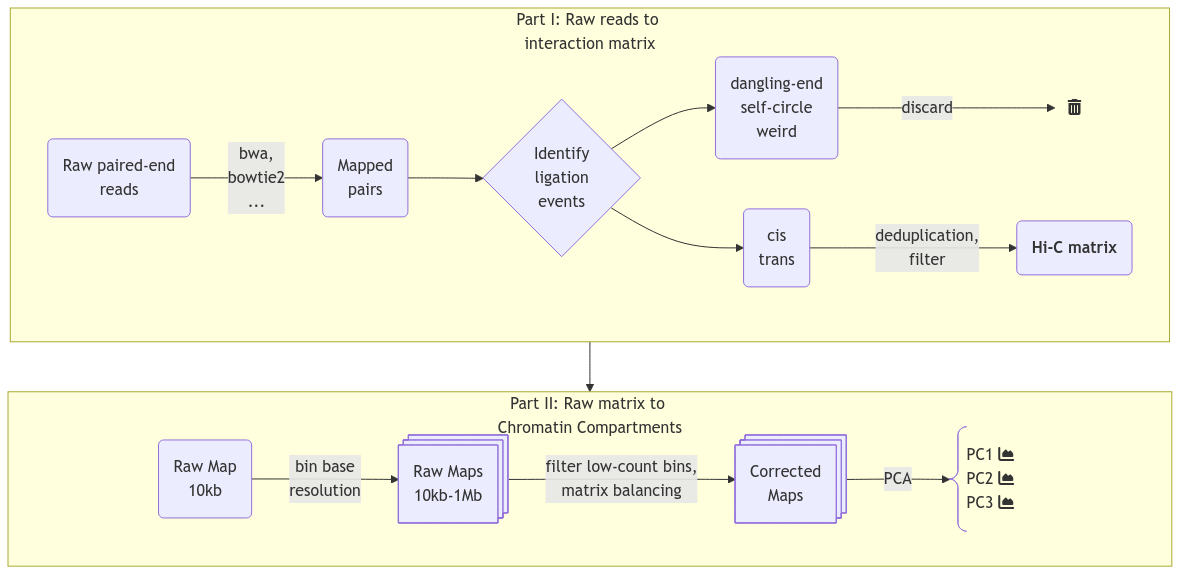
\includegraphics[keepaspectratio]{illustrations/fig-hic-data-analysis.png}}

}

\caption{\label{fig-hic-analysis-flow}A simplified pipeline for Hi-C
data analysis: from raw reads to a Hi-C interaction matrix. See
Table~\ref{tbl-ligation-events} for details on ligation events.}

\end{figure}%

We must align the reads to the reference in such a way that the
\emph{intentional} chimeric read-pairs (as per above-mentioned protocol)
are rescued, and \emph{unintentional} read-pairs are discarded. That is,
we must make sure they represent ligation junction of adjecent chromatin
segments, and not technical artefacts or unintentional (random) fusions
of unrelated DNA.

\subsubsection{Aligning the Hi-C reads}\label{aligning-the-hi-c-reads}

The main difference between Hi-C libraries and standard paired-end
libraries is the high fraction of chimeric reads in Hi-C. As a contact
pair is crosslinked and ligated before sequencing, chimeric reads occur
as a feature, and standard mapping techniques seeks to filter out this
type of reads {[}ref{]}. Thus, we need specialized tools for rescuing
chimeric reads. That said, we have to be cautious distinguishing the
intended chimerism for Hi-C and that of technical artefacts. Any
software for local alignment can be used for aligning reads from a Hi-C
library. However, one should make sure to disable paired-end rescue mode
if possible, otherwise each read in a pair (each mate) should be aligned
separately (Lajoie, Dekker, and Kaplan 2015). This removes the
assumption that the distance between mates fits a known distribution
because the genomic sequences originate from a continuous DNA-fragment.
For example, the \emph{bwa-mem} {[}ref{]} implementation of this (the
\texttt{-P} option) activates the Smith-Waterman algorithm to rescue
missing hits, but disables the search of hits that fit a `proper' pair.
After alignment, each read is typically assigned to the nearest
restriction fragment to enable categorization of pairs into different
categories.

Interestingly, this last step is not included by default in
\emph{pairtools}, as {[}ref{]} observe very similar statistical
properties on pairs that are either close or distant from the nearest
restriction site. Thus, restriction fragment filters are not needed, and
in stead, a simple filter is applied against short-distance pairs that
is automatically calibrated.

\subsubsection{Identifying and Storing Valid Hi-C
Pairs}\label{identifying-and-storing-valid-hi-c-pairs}

One should be cautious when filtering invalid from valid pairs, as they
are not easily distinguished. A ligation event will be categorized into
one of five categories (see Table~\ref{tbl-ligation-events}):
\emph{dangling-end}, \emph{self-circle}, \emph{weird},
\emph{intrachromosomal} (cis), and \emph{interchromosomal} (trans)
(Bicciato and Ferrari 2022, Ch. 1). Either \emph{dangling-end} or
\emph{self-circle} events are reported if a read-pair maps to the same
restriction fragment depending on the orientation, and deemed
uninformative (Lajoie, Dekker, and Kaplan 2015). Usually, \emph{weird}
events are demeed uninformative as well, as it is challenging to
distinguish a sequencing error from the result of a diploid fragment.
PCR duplicates should be discarded as well, having either identical
genomic sequence, or sharing exact 5' alignment positions of the pair
(Lajoie, Dekker, and Kaplan 2015; Bicciato and Ferrari 2022, Ch. 1). The
probability that such pairs are valid (i.e.~there are multiple of the
same pairs) is very low. We also have to distinguish between molecules
with only a single ligation event (one-way contact) or multiple ligation
events (multi-way contacts). For that, a descision should be made on
whether to 1) discard molecules with multiple ligations, 2) report one
of the ligations (e.g.~the 5'-most in both directions), or 3) report all
events on a molecule.

\small

\begin{longtable}[]{@{}
  >{\raggedright\arraybackslash}p{(\linewidth - 2\tabcolsep) * \real{0.2083}}
  >{\raggedright\arraybackslash}p{(\linewidth - 2\tabcolsep) * \real{0.7917}}@{}}
\caption{Five categories of ligation events and a short explanation.
\emph{Hi-C Data Analysis: Methods and Protocols Ch.
1}.}\label{tbl-ligation-events}\tabularnewline
\toprule\noalign{}
\begin{minipage}[b]{\linewidth}\raggedright
Event name
\end{minipage} & \begin{minipage}[b]{\linewidth}\raggedright
Explanation
\end{minipage} \\
\midrule\noalign{}
\endfirsthead
\toprule\noalign{}
\begin{minipage}[b]{\linewidth}\raggedright
Event name
\end{minipage} & \begin{minipage}[b]{\linewidth}\raggedright
Explanation
\end{minipage} \\
\midrule\noalign{}
\endhead
\bottomrule\noalign{}
\endlastfoot
Dangling-end & Non-digested collinear fragments. Fraction can be
high. \\
Self-circle & Collinear fragment(s) have circularized. Very low fraction
could indicate unsuccesful ligation. \\
Weird & Mates have the same orientation on the reference. Is not
possible with single copy fragment. Either sequencing errors or diploid
fragments\footnote{Bicciato and Ferrari (2022) mentions that this type
  of ligations had been used to model interaction between
  sister-chromatids post-replication in \emph{Drosophila}.}. \\
Cis & Pairs from the same chromosome (intrachromosomal) \\
Trans & Pairs from distinct chromosomes (interchromosomal) \\
\end{longtable}

\normalsize

\subsubsection{Quality Control and Interaction
Matrices}\label{sec-matrix-qc}

To determine the quality of the Hi-C library, most tools generate
quality control log files at some point during the filtering steps,
which can then be aggregated and analyzed (with e.g.~MultiQC {[}ref{]}).
The ratios between the different ligation events can be informative
about the quality of the Hi-C library. Here, both the distribution of
discarded reads across categories, as well as the ratios between
\emph{cis}/\emph{trans} interactions for a certain organism provide
information about the library. For example, the biases of different
aligners might be captured by comparing the reason why reads are
discarded between two different aligners, as well as if there is a
preference of \emph{cis} or \emph{trans} in an aligner itself. This
allows for evaluating the mapping parameters as well as the filters
applied downstream. Additionally, \(P(s)\), the contact probability as a
function of genomic separation can be inspected as it should decay with
increasing distance. The \emph{trans}/\emph{cis}-ratio can sometimes be
a good indicator of the noise level in the library, and additionally,
the level of random ligation events can be quantified by counting the
number of \emph{trans} events occurring to mitochondrial genome. They
should not occur naturally, as the mitochondrial genome is separated
from the DNA in the nucleus. This method has some pitfalls that should
be controlled for; some parts of the mitochondrial genome can be
integrated into the host genome, and mitochondrial count may differ
between cell-stages.

Typically, a filter against low mapping quality is applied on the data
before constructing the interaction matrix (Hi-C matrix), and a
conventional threshold is \(mapq < 30\) (Bicciato and Ferrari 2022).
However, a considerable amount of reads do not pass that threshold, and
thus we risk discarding potential valid information and should make sure
to have enough data. Consequently, \emph{HicExplorer} defaults a lower
threshold (\(mapq < 15\)), and \emph{pairtools} enforces no filter by
default, but recommends setting this manually (starting at
\(mapq < 30\)).

A Hi-C interaction matrix simply maps the frequency of interactions
between genomic positions in a sample. The maximum resolution of a Hi-C
matrix is defined by the restriction enzyme, where the size of the
restriction site (probabilistically) determines average space between
each cut. With a 4 bp restriction site, the fragments will average
\(4^4 = 256 bp\) and similarly \(4^6 = 4096 bp\) for a 6 bp restriction
site. This leads to \textasciitilde12,000,000 and \textasciitilde800,000
fragments, respectively. Very deep sequencing is required to achieve
enough coverage to analyze the interaction matrix at the restriction
fragment resolution, but, usually, such high resolution is not required.
Therefore, it is practice to bin the genome into fixed bin sizes, which
also enables a more efficient handling of the data if the full
resolution is not needed (e.g.~when plotting large regions such as a
whole chromosome). The conventional format to store a Hi-C matrix,
consisting of large multidimensional arrays, is HDF5. Each HDF5 file can
store all resolutions and metadata about the sample, resolutions
typically ranging from 10kb to 1Mb. Typically, the stored resolutions
should be multiples of the chosen base-resolution, as the lower
resolutions are constructed by recursive binning of the base resolution.
\emph{cooler} {[}ref{]} neatly offers efficient storage with sparse,
upper-triangle symmetric matrices and naming-conventions of the groups
in their \emph{.h5}-based file format, \emph{.cool}, and they provide a
Python class \texttt{Cooler} as well for efficiently fetching and
manipulating the matrices in Python.

\subsubsection{Inferring from the matrix (Calling
Compartments)}\label{inferring-from-the-matrix-calling-compartments}

The raw frequency matrices are generally not very informative, as the
contact frequencies vary greatly between bins and contain biases in
addition to the \(P(s)\) decay, which results in a diagonal-heavy matrix
with high amount of noise the further we travel from the diagonal.
Therefore, to analyze the three-dimensional structure of the chromatin,
a method for correcting (or balancing) the raw Hi-C matrix has to be
applied. It is unadvisable to correct low-count bins as it will greatly
increase the noise, or to correct very noisy bins, or very high-count
bins. Therefore, some bin-level filters are applied before balancing
(Lajoie, Dekker, and Kaplan 2015);

\begin{itemize}
\tightlist
\item
  Low-count bins are detected by comparing bin sums to the distribution
  of bin sums with a percentile cutoff,
\item
  Noisy bins are detected by comparing bin variance to the variance
  distribution of all bins (and percentile cutoff), and
\item
  Outlier point-interactions are removed (a top-percentile of bin-bin
  interactions)
\end{itemize}

A widely used balancing method is Iterative Correction and
Eigendecomposition (ICE) (Imakaev et al. 2012), which utilizes a
data-driven approach for correcting multiplicative biases. Briefly, is
based on an assumption of equal visibility of all loci, and uses the
pairwise and genome-wide structure to generate a set of biases along
with a map of relative interaction frequencies by iteratively dividing
each row, then each column, by its mean until convergence. This results
in a uniform coverage profile (corrected coverage), yielding a smoother
interaction matrix with slower transitions, thus greatly reduces
visibility-induced biases. It does not distinguish between the sources
of biases, and thus calculates a collective bias for each position.
Imakaev et al. (2012) show that \emph{known} biases are factorizable by
comparing their results to predictions of restriction fragment biases,
GC content, and mappability from a computationally intensive
probabilistic approach. By showing that the product of those known
biases explain \(>99.99%
\) of the variability in their bias estimation, they argue both known
and unknown biases will be captured with their iterative correction
method (also denoted \emph{matrix balancing}).

Even with a binned, filtered, and balanced matrix, we are still left
with the challenge of translating the matrix into biologically relevant
inferations. Importantly, we have to remember that the matrix arise from
a collection of cells and that the interaction frequency cannot be
translated to a fraction of cells. Additionally, the effect from
averaging interaction patterns can cause both individual patterns to be
burried and the average pattern to show a pattern that does not exist in
any of the single cells. Therefore, when pooling matrices one must make
sure that the samples are as similar as possible (e.g.~the same
differentiation stage and so on). We can also not distinguish
interactions that either co-occur in the same cell or ones that are
mutually exclusive. Lastly, the way interaction patterns are defined
poses a challenge; we define the chromatin compartments to be the output
of a method, the `E' in `ICE', eigendecomposition, not as a specific
pattern that we can explicitly search for. Although experimentally
verified to tightly correlate with chromatin states, the inferred
compartments vary with different methods of calculating the eigenvector,
as dicussed in Section~\ref{sec-methods-eigendecomposition} and
Section~\ref{sec-results-eigenvectors}. To further complicate the
challenge, interaction patterns on different scales co-exist and are
difficult to disentangle without simplifying assumptions such as
small-scale interactions are not visible (or they are negligible) at a
certain resolution, or restricting the viewframe to eliminate
large-scale variance between chromosome arms. It is by definition a
speculative exercise to interpret the biological relevance of an
observed pattern, but the consensus is to call compartments on
interacting regions that arise from the eigendecomposition of a Hi-C
matrix without further modifications (Lajoie, Dekker, and Kaplan 2015).
As the eigenvector is only unique up to a sign, a phasing track is used
to orient the eigenvector, aiming for a positive correlation with GC
content (in mammals), making A-compartments represent the active
euchromatin, and B-compartments the closed heterochromatin.

\subsubsection{Compartment Edges and Genomic
Intervals}\label{compartment-edges-and-genomic-intervals}

As arbitrary as a compartment may be defined, we chose to define another
genomic interval for analysis. It is well (Bicciato and Ferrari 2022,
Ch. 3) known that CTCF and other structural proteins preferentially
binds to Topologically Associating Domains (TADs; they were initially
defined as sub-Mb chromatin structures (Lajoie, Dekker, and Kaplan
2015), but now the definition seems to vary based on the method of
extraction {[}ref cooltools{]}). Derived from this, we define a
transition zone between A/B compartments to look for enrichment of
specific regions of interest.

We can test if two sets of genomic intervals correlate (say, compartment
edges and ECH regions) by either proximity of the non-intersecting parts
of the sets, or by intersection over union (Jaccard index). When the
underlying distribution of a statistic (or index) is unknown, a
widespread method in bioinformatics for estimating a p-value is by
bootstrapping. Here, one of the sets are bootstrapped (the intervals are
placed at random positions) a number of times, \(b\), and the fraction
of statistics more extreme than the one we observe is reported as the
p-value.

\section{Reproducibility
Infrastructure}\label{reproducibility-infrastructure}

\textbf{First, describe the importance of reproducibility and the
scientific method. Include a bit of scientific skeptiscism of there is
time.}

Thus, apart from the biological questions we seek to investigate and
answer in this thesis, a major goal of the thesis is to create fully
(and easily) reproducible results through a self-contained and
version-controlled pipeline using git {[}ref{]}, GitHub {[}ref{]},
quarto {[}ref{]}, Conda {[}ref{]}, gwf {[}ref{]}, and Jupyter {[}ref{]}.
See Table~\ref{tbl-reproducibility} for a brief introduction.

\small

\begin{longtable}[]{@{}
  >{\raggedright\arraybackslash}p{(\linewidth - 2\tabcolsep) * \real{0.1944}}
  >{\raggedright\arraybackslash}p{(\linewidth - 2\tabcolsep) * \real{0.8056}}@{}}
\caption{Overview of the tools used for reproducibility of this
thesis.}\label{tbl-reproducibility}\tabularnewline
\toprule\noalign{}
\begin{minipage}[b]{\linewidth}\raggedright
Tool
\end{minipage} & \begin{minipage}[b]{\linewidth}\raggedright
Description
\end{minipage} \\
\midrule\noalign{}
\endfirsthead
\toprule\noalign{}
\begin{minipage}[b]{\linewidth}\raggedright
Tool
\end{minipage} & \begin{minipage}[b]{\linewidth}\raggedright
Description
\end{minipage} \\
\midrule\noalign{}
\endhead
\bottomrule\noalign{}
\endlastfoot
Jupyter & Interactive coding environment for analysis and development
(notebooks are natively rendered with Quarto) \\
Quarto & A Quarto Manuscript project nested inside a Quarto Book for
rendering html (website) and PDF (manuscript) from Markdown via Pandoc.
Supports direct embedding of output from Jupyter Notebook cells (plots,
tables). \\
Conda & For managing software requirements and dependency versions
reproducibly. \\
git & Version control and \texttt{gh-pages} branch for automated render
of Quarto project \\
GitHub & Action was triggered \texttt{on\ push} to render the project
and host on
\href{https://munch-group.org/hic-spermatogenesis/}{munch-group.org} \\
\emph{gwf} & Workflow manager to automate the analysis on a HPC cluster,
wrapped in Python code. \texttt{workflow.py} currently does everything
from \texttt{.fastq} to \texttt{.cool}, but notebooks can be set to run
sequentially as part of the workflow as well. \\
\end{longtable}

\normalsize

\subsection{GWF: workflow management for High-Performance Computing
(HPC)}\label{gwf-workflow-management-for-high-performance-computing-hpc}

To enable consistently reproducing the analyses, a workflow manager is
used. Several exist, but the most well-known must be \emph{snakemake}
{[}ref{]}. However, we use the pragmatic (their own words), lightweight
workflow manager \emph{gwf}, which is optimized for the GenomeDK
insfrastructure, and has the benefit of in-house support.

Briefly, \emph{gwf} works on a python script, conventionally
\texttt{workflow.py}, that wraps all the jobs (\emph{targets} in gwf
lingo) you will submit to the HPC cluster. Each target is submitted from
a template, written as a Python function, which includes \texttt{inputs}
and \texttt{outputs} that \emph{gwf} should look for when building the
depency graph, \texttt{options} list of resources that is forwarded to
the queueing system (\emph{Slurm} in our case), and \texttt{specs},
specifying the submission code in Bash as a formatted Python string
(meaning we can pass Python variables to the submission code), providing
an extremely flexible framework for running large and intensive analyses
in a high-performance computing environment.

\subsection{Project Initialization}\label{project-initialization}

\subsubsection{\texorpdfstring{\emph{gwf}}{gwf}}\label{gwf}

The initialization of the project directory is the basis of
reproducibility and transparency, together with \texttt{workflow.py}
inhabiting the main directory. Specifically, it includes a subdirectory
for (intermediate) files that are produced by the pipeline,
\texttt{steps/}. Everything in this directory is reproducible simply by
re-running the \emph{gwf}-workflow. It is thus not tracked by
\texttt{git}, as the large files (raw reads, aligned read-pairs, etc.)
it contains are already indirectly tracked (\texttt{workflow.py} is
tracked). It can be safely deleted if your system administrator tells
you to free up disk space, although you would have to run the workflow
again to continue the analysis. Several directories are created for
files that are not produced by the pipeline, that is, files that the
workflow uses, configuration files, figures edited by hand, etc.
Ideally, as few files as possible should be outside of \texttt{steps/},
to be as close as possible to an automated analysis.

\subsubsection{Jupyter Notebooks}\label{jupyter-notebooks}

A \texttt{notebooks/} subdirectory contains Jupyter notebooks that are
named chronologically, meaning they operate on data located in either
\texttt{steps/} or generated from a previous notebook. This way, the
workflow can also be set up to run the notebooks (in order) to produce
the figures, tables, and their captions used in this manuscript.

\subsubsection{Quarto}\label{quarto}

Quarto is an open-source scientific and technical publishing system that
uses (pandoc) markdown to create and share production quality output,
integrating Jupyter Notebooks with Markdown and LaTeX and enabling
embedding content across \emph{.ipynb} and \emph{.qmd}. In \emph{.qmd},
code chunks in several programming languages can be executed and
rendered, including Python, R, mermaid (JavaScript-based diagramming). A
Quarto project is configured with a YAML configuration file
(\texttt{\_quarto.yml}) that defines how output is rendered. In this
project, we use a nested structure, nesting a \emph{Slides} project and
a \emph{Manuscript} project inside a \emph{Book} project. To manage the
directory as a Quarto Book project, a quarto configuration file was
placed at the base, defining how the Book should be rendered.
Additionally, configuration files were placed in \texttt{slides/} and
\texttt{thesis/}, to render them as Quarto Slides and Quarto Manuscript,
respectively. This nested structure lets us render different subprojects
with different configurations than the main project, for example to
generate the manuscript, a single Quarto Markdown file, in both
\emph{.html} and \emph{.pdf}, and only including embedded outputs from
specified cells from notebooks in the parent directory. Although the
Quarto framework is extensive, it is still under development and has
several drawbacks worth mentioning. First, one can only embed the output
of code cells from notebooks, meaning the only way to embed text with a
python variable (e.g.~you want the manuscript to reflect the actual
value of a variable, sample sizes
\texttt{n\ =\ {[}1000,\ 10000,\ 100000{]}}, and their respective
outputs) is by converting a formatted python string into Markdown and
send it to the output. Second, embedded figures will be copied as-is in
the notebook, and thus cannot be post-processed with size or layout.
This makes it impractical to e.g.~use the same figures in slides and in
the manuscript. Third, when rendering large projects that is tracked by
git, some output files (that have to be tracked to publish the website)
can exeed GitHub size limits. Especially if rendering in the \emph{jats}
format, producing a MECA Bundle that should be the most flexible way to
exchange manuscripts {[}ref{]}. However, as not applicable to this
thesis, the option was simply disabled. Fourth, some functionality
relies on external dependencies that cannot be installed on a (linux)
remote host (GenomeDK), such as relying on a browser for converting
\texttt{mermaid} diagrams into png for the pdf-manuscript.

\subsection{git and GitHub}\label{git-and-github}

To track the project with git and GitHub, the abovementioned structure
was initialized as a GitHub repository, including a workflow for GitHub
Actions to publish and deploy the website on the \texttt{gh-pages}
branch when pushing commits to \texttt{main}. Briefly, it sets up a
virtual machine with Quarto and its dependencies, renders the project as
specified in the \texttt{\_quarto.yml} configuration file(s), and
publishes the project on the group website
\href{https://munch-group.org/hic-spermatogenesis}{munch-group.org}.

\section{Our research question}\label{our-research-question}

In this project, we formulate two main objectives:

\subsubsection{A}\label{a}

Redo the Hi-C analyses from (Wang et al. 2019) using the latest macaque
reference genome, \emph{rheMac10}, with some modifications. We decided
to use \emph{HiCExplorer}, a Python-based software for command line use,
and supplement the analyses with the \emph{Open2C Ecosystem} ({``Open
{Chromosome Collective} ({Open2C})''} n.d.) that have a Pyton API as
well as command-line functions, which can be paired very well with
Jupyter Notebooks. The majority of the data analysis was run with a
\emph{gwf} workflow, and the commands that were visually inspected were
run in Jupyter Notebooks.

\subsubsection{B}\label{b}

Compare with regions of extended common haplotypes (strong selective
sweeps) that are found in \emph{human}, and with regions of negative
selection of minor parent ancestry in baboons. Investigate the
biological meaning of the results. We use in-house software to compare
genomic intervals.

\chapter{Methods}\label{methods}

All computations were performed on GenomeDK (GDK) {[}ref{]}, an HPC
cluster located on Aarhus Uninversity, and most of the processing of the
data was made into a custom \emph{gwf} workflow {[}ref{]}, a workflow
manager developed at GDK. I would like to thank GDK and Aarhus
University for providing computational resources and support that
contributed to these research results.

With the analysis tools determined in the above section, we decided it
was not feasible to follow the exact approach as Wang et al. (2019) with
any of \emph{HiCExplorer} and \emph{Open2C}, as they use a third
software, \emph{HiC-Pro}. For mapping the raw reads, Hic-Pro internally
uses bowtie2 in end-to-end mode, followed by trimming the 3'-end of the
unmapped reads, then remapping the 5'-ends to rescue chimeric fragments.
I mapped the reads using \texttt{bowtie2\ -\/-end-to-end} without the
rescue-remapping, and it returned a very high fraction of discarded
reads, and it would be silly to spend time on implementing the remapping
approach manually. When redoing analyses, it is not sensical to use
methods that are not state-of-the-art, and judged by the time since last
release (HiC-Pro v3.1.0 in 2021), both HiCExplorer and Open2C are more
recent. Additionally, the HiC-Pro pipeline stops at a normalized contact
map, and is thus not sufficient for downstream analysis. In hindsight,
it would have been more sensical to use \emph{HiC-Pro} to get normalized
contact maps, then continue analyzing with
\emph{cooler}/\emph{cooltools}, then compare the results evenly with the
results achieved from using Open2C from start to finish.
Figure~\ref{fig-hic-tools-comparison} gives an overview of the 3
pipelines metioned in this report.

\begin{figure}

\centering{


\includegraphics[width=0.5\linewidth,height=3\textheight]{illustrations/placeholder2000x360.png}

}

\caption{\label{fig-hic-tools-comparison}A 3-column flow of HiC-Pro,
HiCExplorer, and Open2C}

\end{figure}%

\section{Fetching raw data}\label{fetching-raw-data}

To reproduce the results from (Wang et al. 2019), I chose to use their
raw data directly from the SRA portal {[}ref{]}. I filtered the data to
contain all their paired-end Hi-C reads, and included only macaque
samples. The data set also contains RNAseq data, and the same tissues
for both macaque and mouse. The meta data for the data set was extracted
into a runtable \texttt{SRA-runtable.tsv}. To get an overview of the
data accessions used in this analysis, we will first summarize the
runtable that contains the accession numbers and some metadata for each
sample (Table~\ref{tbl-runtable-summary}). It adds up to
\textasciitilde1Tb of compressed \texttt{fastq} files, holding
\textasciitilde9.5 billion reads, roughly evenly spread on the 5 tissue
types.

\small

\begin{longtable}[]{@{}lllll@{}}

\caption{\label{tbl-runtable-summary}Summary of the data accessions used
in this analysis}

\tabularnewline

\toprule\noalign{}
& source\_name & GB & Bases & Reads \\
\midrule\noalign{}
\endhead
\bottomrule\noalign{}
\endlastfoot
0 & fibroblast & 211.403275 & 553,968,406,500 & 1,846,561,355 \\
1 & pachytene spermatocyte & 274.835160 & 715,656,614,700 &
2,385,522,049 \\
2 & round spermatid & 243.128044 & 655,938,457,200 & 2,186,461,524 \\
3 & sperm & 164.131640 & 428,913,635,400 & 1,429,712,118 \\
4 & spermatogonia & 192.794420 & 518,665,980,300 & 1,728,886,601 \\

\end{longtable}

\normalsize

\subsection{Fetching and indexing the
reference}\label{fetching-and-indexing-the-reference}

Wang et al. (2019) use the 2006-version of the macaque reference,
\emph{rheMac2}. Supporting my previous sentiment about not using
outdated resources I find it reasonable to use the latest reference,
\emph{rheMac10}. Warren et al. (2020) have improved contiguity from
\emph{rhemac8} by 120 fold, going from N50 contig size of 107 Kbp to 46
Mbp. Part of the reasoning for reproducing their results was doing so on
the latest assembly of the \emph{Macaca mulata} genome, which arguably
will result in a more accurate mapping of the reads, and a better
inference of the chromatin compartments as well.

Therefore, the latest reference genome for rhesus macaque/\emph{Macaca
mulata}, \emph{rheMac10}/\emph{Mmul\_10} (UCSC or NCBI naming
conventions, respectively) was downloaded to GDK from UCSC web servers
with \texttt{wget}. To use \texttt{bwa} for mapping, rheMac10 needs to
be indexed with both \texttt{bwa\ index} with the \texttt{-\/-bwtsw}
option and \texttt{samtools\ faidx}, which results in six indexing files
for \texttt{bwa\ mem} to use.

Several mappers were used in different configurations (described in
below), and \texttt{bowtie2} requires its own indexing of the reference,
using \texttt{bowtie2-build\ -\/-large-index}, which creates six index
files for \texttt{bowtie2} to use. \texttt{-\/-large-index} creates the
special indexing format required for large genomes such as macaque.

\section{HiCExplorer trials}\label{hicexplorer-trials}

To get aligned reads in a format compatible with HiCExplorer, the read
mates have to be mapped individually to the reference genome. This
supports the old convention to avoid the common heuristics of local
aligners used for regular paired-end sequencing libraries (Lajoie,
Dekker, and Kaplan (2015)). HiCExplorer provide examples for both
\emph{bwa} and \emph{bowtie2}, so I used both with recommended settings.
\emph{bowtie2} was more resource-intensive, and only succesfully aligned
a small fraction of the reads {[}ref sup-fig-bowtie2-stats{]}, but
likely some parameters could be tuned for better alignment. In both
cases, the aligner outputs a .bam-file for each mate
(\texttt{sample\_R1.bam} and \texttt{sample\_R2.bam}), and HiCExplorer
performs the parsing, deduplication, and filtering of the reads and
builds the raw interaction matrix in a single command,

\texttt{hicBuildMatrix\ -s\ sample\_R1.bam\ sample\_R2.bam\ -o\ matrix.h5\ {[}...{]}},

For parsing, the command needs a \texttt{restrictionCutFile}, locating
the restriction sites from the restriction enzyme used on the reference
genome, which is generated with \texttt{hicFindRestSites} that operates
on the reference genome and restriction sequence. The default filter,
\texttt{-\/-minMappingQuality\ 15}, was applied as described in
Section~\ref{sec-matrix-qc}. Notably, HiCExplorer has no options on
handling multiple ligations, and thus the method is unknown. I assume
that they have the intitial design of Hi-C libraries in mind.

\begin{figure}

\centering{


\includegraphics[width=0.7\linewidth,height=1\textheight]{illustrations/placeholder2000x360.png}

}

\caption{\label{fig-hicexplorer-workflow}Overview of the target
templates used for hicexplorer. As most operations are handled by
\texttt{hicBuildMatrix}, it is rather simple.}

\end{figure}%

\small

\begin{longtable}[]{@{}lllll@{}}

\caption{\label{tbl-hic-exploration}The samples chosen for initial data
exploration with HiCExplorer. From NCBI SRA Portal.}

\tabularnewline

\toprule\noalign{}
& Run & Bases & Bytes & source\_name \\
\midrule\noalign{}
\endhead
\bottomrule\noalign{}
\endlastfoot
0 & SRR6502335 & 73201141800 & 31966430779 & fibroblast \\
1 & SRR6502336 & 65119970100 & 24433383054 & fibroblast \\
2 & SRR6502337 & 52769196300 & 23015357755 & fibroblast \\
3 & SRR6502338 & 52378949100 & 22999581685 & fibroblast \\
4 & SRR6502339 & 28885941600 & 10960123150 & fibroblast \\

\end{longtable}

\normalsize

For the initial exploration of methods with \emph{HiCExplorer}, we chose
five fibroblast samples (see Table~\ref{tbl-hic-exploration}). The goal
was to replicate some of the figures from Wang et al. (2019) using
\emph{HiCExplorer}, especially to reconstruct interaction matrices and
E1 graphs from macaque data. We constructed matrices with
\texttt{hicBuildMatrix} as described from the separately mapped
read-pairs. Along with the matrix \emph{.h5} file, a \emph{.log} file
was created as well, documenting the quality control for the sample.
Multiple logs were aggregated and visualized with \texttt{hicQC}.

Before correction (or balancing) of the interaction matrix, a
pre-correction filter is applied, filtering out low-count bins and very
high-count bins. A threshold for Mean Absolute Deviation (\emph{MAD}) is
estimated by \texttt{hicCorrect\ diagnostic\_plot}, followed by
iterative correction with
\texttt{hicCorrect\ correct\ -\/-correctionMethod\ ICE}. The PCA was
performed with \texttt{hicPCA} on the corrected matrices, yielding the
first 3 PCs.

\texttt{hicPlotMatrix} plots matrices directly to .png (no display).
When keeping the analysis in a Jupyter Notebook (using the builtin
shell-escape commands to execute \texttt{bash} code), the plot files
must be embedded back into the notebook. There is limited support for
modifying the plot (from command-line options), such as to add spacing
for a bigWig track with E1 values, add plot titles, and define the size
and resolution of the plot. I briefly tried to implement a plotting
function on the .h5 matrices and bigWig tracks, but it could not fetch
regions from a matrix on the fly and had to load the full matrix into
memory (that is, all full-length chromosomes).

\section{Open2C pipeline}\label{open2c-pipeline}

\begin{figure}

\centering{

\pandocbounded{
\includegraphics[keepaspectratio]{illustrations/placeholder2000x360.png}}

}

\caption{\label{fig-flowchart-handling-coolers}Showing the \emph{gwf}
target templates used with the \emph{Open2C} pipeline. As it is highly
modular, it is also a bit elaborate.}

\end{figure}%

A \emph{gwf} workflow was created to handle the first part of the data
processing, and each accesion number (read pair, mate pair) from the
Hi-C sequencing was processed in parallel, so their execution was
independent from each other.

\subsubsection{Downloading the reads}\label{downloading-the-reads}

The reads were downloaded from NCBI SRA with SRA-toolkit (DevTeam 2024)
directly to GDK using a docker image of \texttt{sra-downloader} {[}ref
\emph{wwydmanski/sra-downloader}{]} as gunzipped \texttt{.fastq} files.
Although possible to provide a list of accessions to the toolkit, I
submitted each accession as a separate target, as \texttt{SRA\ Toolkit}
acts sequentially, and only starts the next download after all
compression tasks were done. It was therefore a low-hanging fruit to
parallelize the download for efficiency.

\subsubsection{Mapping Hi-C reads}\label{mapping-hi-c-reads}

Suspiciously, ({``Open {Chromosome Collective} ({Open2C})''} n.d.) never
mentions any problems with aligning the Hi-C reads, they just provide an
example using \texttt{bwa\ mem} in paired-end mode and with the
\texttt{-P} option set, which activates the Smith-Waterman {[}ref{]}
algorithm to rescue missing hits, by focusing on assigning only one of
the mates to a good mapping and escape mate-rescue. The documentation of
\texttt{bwa} \href{https://bio-bwa.sourceforge.net}{ref} state that both
bwa-mem and bwa-sw will rescue chimeric reads. Consequently, Open2C does
not have a builtin way of pairing the reads after mapping, and I was
left with two options: \textbf{1)} to re(-)pair the individually mapped
read-mates (.bam) with \texttt{samtools-fixmate} into one of the
specific input formats required for \texttt{cooler} to create an
interaction matrix \emph{cooler}, or \textbf{2)} re-map the reads using
Open2C's recommendations and use their established pipeline for
producing a cooler. I chose the latter, where I mapped the fastq files
to \emph{rheMac10} in paired end mode for a pair (\(m1\), \(m2\)) with
\texttt{bwa\ mem\ -SP\ rheMac10\ m1\ m2}.

\subsubsection{Parse and sort the reads}\label{parse-and-sort-the-reads}

We need to convert the alignments into ligation events, and distinguish
between several types of ligation events. The simplest event is when
each side only maps to one unique segment in the genome `UU'. Other
events, where one or both sides map to multiple segments or the reads
are long enough (\textgreater150bp) to contain two alignments (multiple
ligations) have to be considered as well. Multiple ligations (reads that
have multiple ligation sites, thus having several valid alignments to
the reference) are called \emph{walks} by Open2C, and are treated
according to the \texttt{-\/-walks-policy} when parsing the alignments
into valid pairs (or valid Hi-C contacts). Here, \texttt{mask} is the
most conservative and masks all complex walks, whereas \texttt{5unique}
and \texttt{3unique} reports the 5'-most or 3'-most unique alignment on
each side, respectively, and \texttt{all} reports all the alignments.
The pairs are piped directly into \texttt{pairtools\ sort} after
parsing, as the deduplication step requires a sorted set of pairs. The
\emph{.pairs}-format produced by \texttt{pairtools} is an extension the
\href{https://data.4dnucleome.org/file-formats/pairs/}{4DN
Consortium}-specified format, storing Hi-C pairs as in
Table~\ref{tbl-pairsformat}.

\small

\begin{longtable}[]{@{}
  >{\raggedleft\arraybackslash}p{(\linewidth - 4\tabcolsep) * \real{0.1644}}
  >{\raggedright\arraybackslash}p{(\linewidth - 4\tabcolsep) * \real{0.1644}}
  >{\raggedright\arraybackslash}p{(\linewidth - 4\tabcolsep) * \real{0.6712}}@{}}
\caption{Column specification of the .pairs format as extended by
\texttt{pairtools} {[}ref{]}.}\label{tbl-pairsformat}\tabularnewline
\toprule\noalign{}
\begin{minipage}[b]{\linewidth}\raggedleft
Index
\end{minipage} & \begin{minipage}[b]{\linewidth}\raggedright
Name
\end{minipage} & \begin{minipage}[b]{\linewidth}\raggedright
Description
\end{minipage} \\
\midrule\noalign{}
\endfirsthead
\toprule\noalign{}
\begin{minipage}[b]{\linewidth}\raggedleft
Index
\end{minipage} & \begin{minipage}[b]{\linewidth}\raggedright
Name
\end{minipage} & \begin{minipage}[b]{\linewidth}\raggedright
Description
\end{minipage} \\
\midrule\noalign{}
\endhead
\bottomrule\noalign{}
\endlastfoot
1 & read\_id & the ID of the read as defined in fastq files \\
2 & chrom1 & the chromosome of the alignment on side 1 \\
3 & pos1 & the 1-based genomic position of the outer-most (5') mapped bp
on side 1 \\
4 & chrom2 & the chromosome of the alignment on side 2 \\
5 & pos2 & the 1-based genomic position of the outer-most (5') mapped bp
on side 2 \\
6 & strand1 & the strand of the alignment on side 1 \\
7 & strand2 & the strand of the alignment on side 2 \\
8 & pair\_type & the type of a Hi-C pair \\
9 & mapq1 & mapq of the first mate \\
10 & mapq2 & mapq of the second mate \\
\end{longtable}

\normalsize

I initially used \texttt{-\/-walks-policy\ mask} without fully
understanding the implications, but knowing it was the most conservative
of the options. Only later I realized the recommendations from
\emph{pairtools}, specifically informing that longer reads (\(>150bp\))
might have a significant proportion of reads that contain complex walks.
With this in mind and as the average read-length of our data is 300 bp,
I decided to re-parse the alignments into a new set of pairs, and
equally apply the recommended filter (next section). As both results are
saved, we can compare the two approaches.

\subsubsection{Filter and deduplicate
pairs}\label{filter-and-deduplicate-pairs}

Pairtools comes with a de-duplication function, \texttt{dedup}, to
detect PCR duplication artefacts. At this point we will remove all reads
that are mapped to an unplaced scaffold. Even though the publication of
\emph{rhemac10} assembly states they have closed 99\% of the gaps since
\emph{rhemac8} {[}ref{]}, \emph{rheMac10} still contain more than 2,500
unplaced scaffolds, which are all uninformative when calculating the
chromatin compartments as is the goal of this analysis. Therefore, we
simply only include the list of conventional chromosomes (1..22, X, Y)
when doing the deduplication. Initially, the default values were used to
remove duplicates, where pairs with both sides mapped within 3 base
pairs from each other are considered duplicates. \texttt{cooler}
recommend to store the most comprehensive and unfiltered list of pairs,
and then applying a filter it on the fly by piping from
\texttt{pairtools\ select}. Initially, I missed this step and I did not
filter for mapping quality. After reparsing the alignments and applying
the same analysis, we compare the two pipelines. A quality control
report is generated by \texttt{pairtools\ dedup} as well, and the
reports are merged and visualized with \texttt{MultiQC} {[}ref{]} for
each cell type.

\subsubsection{Create interaction matrices
(coolers)}\label{create-interaction-matrices-coolers}

The final part of the \emph{gwf} workflow takes \texttt{.pairs} as input
and outputs a \texttt{.cool} file (\emph{cooler}). Initially, we read
directly from the newly generated deduplicated pairs without additional
filtering, but the official recommendation is to filter out everything
below \(mapq = 30\) by piping the pairs through
\texttt{pairtools\ select\ "(mapq1\textgreater{}=30)\ and\ (mapq2\textgreater{}=30)"}
to \texttt{cooler\ cload\ pairs}. I then re-parsed the alignments and
created new coolers, including only the Hi-C contacts where
\(mapq \leq 30\), following the current recommendations from
\emph{cooler}.

\subsubsection{Pooling samples (Merging
coolers)}\label{pooling-samples-merging-coolers}

The samples are grouped into \emph{replicates} with a unique
\textbf{BioSample} ID, but we chose to pool all the interaction matrices
for each cell type. We reason that when Wang et al. (2019) determine
compartments to be highly reproducible between replicates, by merging
the replicates we can get a more robust signal.

\texttt{cooler\ merge} was used to merge all samples in each cell-type
directory to just one interaction matrix for each cell type. The
function merges matrices of the same dimensions by simply adding the
interaction frequencies of each genomic position together, resulting in
less empty or low-count bins.

\subsubsection{Create multi-resolution coolers
(zoomify)}\label{create-multi-resolution-coolers-zoomify}

A feature of working inside the ecosystem of \emph{Open2C} {[}ref{]} is
that it natively provides support for storing sparse interaction
matrices in multiple resolutions in the same file by adding HDF5-groups
to the (multires-)cooler. We can then efficiently store resolutions
(i.e., different bin sizes) that is multiples of the smallest bin size.
We chose to use 10kb, 50kb, 100kb, and 500kb bins, and the resolutions
are made by recursively binning the base resolution. They call this
process zoomifying, and \texttt{cooler\ zoomify} does the job (it
recursively calls \texttt{cooler\ coarsen} to merge bins).

\subsubsection{Matrix balancing (Iterative
correction)}\label{matrix-balancing-iterative-correction}

Finally, we balance (or correct) the matrices using the cooler CLI. We
use \texttt{cooler\ balance} with the default options which iteratively
balances the matrix (Iterative Correction).

We balance the matrices on each resolution, and thus it cannot be done
prior to zoomifying. They (Abdennur and Mirny (2020)) state that the
balancing weights are resolution-specific and will no longer retain its
biological meaning when binned with other weights. Therefore, we apply
\texttt{cooler\ balance} to each resolution separately.
\texttt{cooler\ balance} will create a new column in the \texttt{bins}
group of each cooler, \texttt{weight}, which can then be included or not
in the downstream analysis. This means we will have access to both the
balanced and the unbalanced matrix.

The default mode uses genome-wide data to calculate the weights for each
bin. It would maybe be more suitable to calculate the weights for
\emph{cis} contacts only, and that is possible through the
\texttt{-\/-cis-only} flag, and that can be added to another column, so
that we can compare the difference between the two methods easily.
However, when adding the option, the process seemed to stall and had to
be terminated manually, and it was not investigated further.

\subsubsection{Eigendecomposition}\label{sec-methods-eigendecomposition}

The eigendecomposition of a Hi-C interaction matrix is performed in
multiple steps. As value of the eigenvector is only \emph{significant}
up to a sign, it is convention {[}ref{]} to use GC content as a phasing
track to orient the vector. E1 is arbitrarily defined to be positively
correlated with GC content, meaning a positive E1 value signifies an
active chromatin state, which we denote a A-type compartment (or simply
A-compartment). We performed eigendecomposition of two resolutions, 100
Kbp and 500 Kbp. Wang et al. (2019) briefly describes their method to
calculate the eigenvectors as a sliding window approach on the
observed/expected matrix in 100 kb resolution summing over 400 kb bins
with 100 kb step size, a method I was not able to replicate in the
\emph{Open2C} ecosystem. I decided to mimic this by smoothing the 100 kb
E1 values by summing to 500 kb bins in steps of 100 kb, yielding a
comparable resolution which I denote `\emph{pseudo}-500 kb' resolution
(\emph{ps500kb}).

First, we calculate the GC content of each bin of the reference genome,
\emph{rheMac10}, which is binned to the resolution of the Hi-C matrix we
are handling. It is done with \texttt{bioframe.frac\_gc}
(\emph{Open2C}). To calculate the E1 compartments, we use only
within-chromosome contacts (\emph{cis}), as we are not interested in the
genome-wide contacts. \texttt{cooltools.eigs\_cis} will decorrelate the
contact-frequency by distance before performing the eigendecomposition.
\texttt{eigs\_cis} needs a \emph{viewframe} (view) to calculate E1
values, the simplest view being the full chromosome. However, when there
is more variance between chromosome arms than within arms, the sign of
the first eigenvector will be determined largely by the chromosome arm
it sits on, and not by the chromatin compartments. To mitigate this, we
apply a chromosome-arm-partitioned view of the chromosome (as a bedlike
format, described in \texttt{bioframe} docs {[}ref{]}).

Additionally, to mimic the \emph{Local PCA} from (Wang et al. 2019), I
also defined a view of 10 Mb bins. Thoughout the project, I will compare
results from each of the three views and resolutions.

\subsubsection{Plotting matrices}\label{plotting-matrices}

We use matplotlib and seaborn to plot in the \emph{Open2C} framework.
Utilizing the \texttt{cooler} class, we can fetch regions of the matrix
without modifying the file. As my analysis is centered around the X
chromosome, it is efficiently handled by simply fetching `chrX' from the
matrix with
\texttt{cooler.Cooler.matrix().fetch(\textquotesingle{}chrX\textquotesingle{})}.
Many methods of the cooler class returns data selectors, which do not
retrieve data before it is queried {[}ref{]}. This means we can create
many selectors at once without overflowing memory, enabling us to plot
multiple interaction matrices side-by-side, e.g.~the corrected and
un-corrected matrices. This is easily done with the \texttt{balance}
parameter of the matrix selector (\texttt{.matrix()}), which determines
if it should apply the balancing weights to the coordinates and defaults
to \texttt{True}.

The matrix is retrieved an plotted with
\texttt{matplotlib.pyplot.matshow}, which automatically produces a
heatmap image of the matrix. Here, in stead of transforming the
interaction matrix, the color scale is log-transformed with
\texttt{matplotlib.colors.LogNorm}. Additionally, \texttt{cooltools}
comes with more tools to aid visualization: \emph{adative coarsegrain}
and \emph{interpolation}, which can be chained.
\texttt{adaptive\_coarsegrain} iteratively coarsens an array to the
nearest power of two and refines it back to the original resolution,
replacing low-count pixels with NaN-aware averages to ensure no zeros in
the output, unless there are very large regions that exceed the
\texttt{max\_levels} threshold, such as the peri-centromeric region.

I implemented a plotting utility, \texttt{plot\_for\_quarto} in notebook
\texttt{07\_various\_plotting.ipynb} that is compatible with the YAML
cell-options read by Quarto's \texttt{embed} shortcode. It will take an
arbitrary number of samples and plot a chromosome (or region) with or
without its respective E1 value for either of the three viewframes that
has been created. The input is a (subsetted) \emph{pandas DataFrame},
defined from a file search matching a pattern specified to the
\texttt{glob} Python module.

\subsection{Compartments and Their Edges (Transitional
Regions)}\label{compartments-and-their-edges-transitional-regions}

From the eigenvectors, the A-compartments were extracted in
bedgraph-format
(\texttt{{[}\textquotesingle{}chrom\textquotesingle{},\ \textquotesingle{}start\textquotesingle{},\ \textquotesingle{}end\textquotesingle{}{]}})
and compared with ECH90 regions lifted to \emph{rheMac10} from human
{[}ref what reference?{]}. We perform visual inspection of the genomic
intervals and test whether ECH90 regions are enriched near the edges of
the compartments by defining a 200 kilobase transition-zone centered at
each sign change of E1 (referred to as \emph{compartment edge}). We
compare genomic intervals (or sets) both visually by plotting the
regions, and by a proximity test and bootstrapping the Jaccard index.

\subsubsection{Proximity test}\label{proximity-test}

Determines whether the non-overlapping parts of the sets are more
proximal than expected by chance. We define the \emph{annotation} set
and the \emph{query} set, and the distance from each interval on the
\emph{query} to the most proximal interval on the \emph{annotation} is
used to generate an index of proximity by the mean distance to nearest
interval in the \emph{annotation}. Then, bootstrapping (\(b = 100000\))
is performed by randomly \emph{re}placing the query intervals to
generate the null distribution, and finally, the fraction of the
\emph{null} as or more extreme as our observed proximity is reported as
the p-value.

\subsubsection{Jaccard test}\label{jaccard-test}

Measures the significance of the observed Jaccard index (intersection
over union) between two sets. The index is a measure of
\emph{similarity} (\(intersection/union\)) between two sets (between 0
and 1), which is very sensitive to the size difference between the sets,
as even when comparing a set of intervals to a small subset of itself
will yield a very small Jaccard index. When we use bootstrapping to
generate a null distribution (shuffling the intervals of the
\emph{query}), we find the probability that the two sets (with their
respective number and size of intervals), are as similar or more than
what we observe. The ratio is reported as the p-value. However, this
approach is still sensitive to flipping of query/annotation (if the
reginos are not the same size), as only the query is bootstrapped.

\subsubsection{Multiple testing}\label{multiple-testing}

Careful considerations were made to avoid multiple testing biases
(p-hacking): Performing tests on all combinations of variables (cell
type, resolution, viewframe, flip annot, query) will yield 180 p-values
for each test, and we would have to adjust the significance threshold
(with \(\alpha = 0.05\), we expect 9 `significant' tests by chance
alone). However, if we test only a few combinations we will greatly
reduce that.

\chapter{Results}\label{results}

\section{HicExplorer Trials}\label{hicexplorer-trials-1}

\subsection{Quality Control}\label{quality-control}

The separately mapped read-mates were parsed into a \emph{.h5}
interaction matrix by \texttt{hicBuildMatrix}, which include a
\emph{.log} file documenting the builtin quality control (hereafter,
\emph{QC}). Log files from the 5 samples were merged with \texttt{hicQC}
(Figure~\ref{fig-explorer-qc}). We observe showed equal fractions of the
read-orientation of read-pairs
(Figure~\ref{fig-explorer-read-orientation}), which is expected for a
good Hi-C library. Additionally, it determines between 40\% to 50\% of
the total reads to be valid Hi-C contacts
(Figure~\ref{fig-explorer-unique-pairs}), which is usually only
25\%-40\% (as described in HiCExplorer docs).
Figure~\ref{fig-explorer-contact-distance} shows, however, unusually
high fractions of \emph{inter}-chromosomal contacts (up to 30\%)
compared to \emph{intra}-chromosomal contacts (also denoted \emph{trans}
and \emph{cis} contacts, respectively). It is expected that \emph{cis}
contacts are orders of magnitude more frequent than \emph{trans}
contacts (Bicciato and Ferrari 2022, 2301:236; Lieberman-Aiden et al.
2009), and HiCExplorer states it should be below 10\% (docs). The high
fraction may be mitigated by enforcing a stricter \emph{mapq} threshold
for a valid Hi-C pair, as we also observe higher-than expected valid
contacts. However, we continue without the current matrices.

\begin{figure}

\begin{minipage}{0.33\linewidth}

\centering{

\pandocbounded{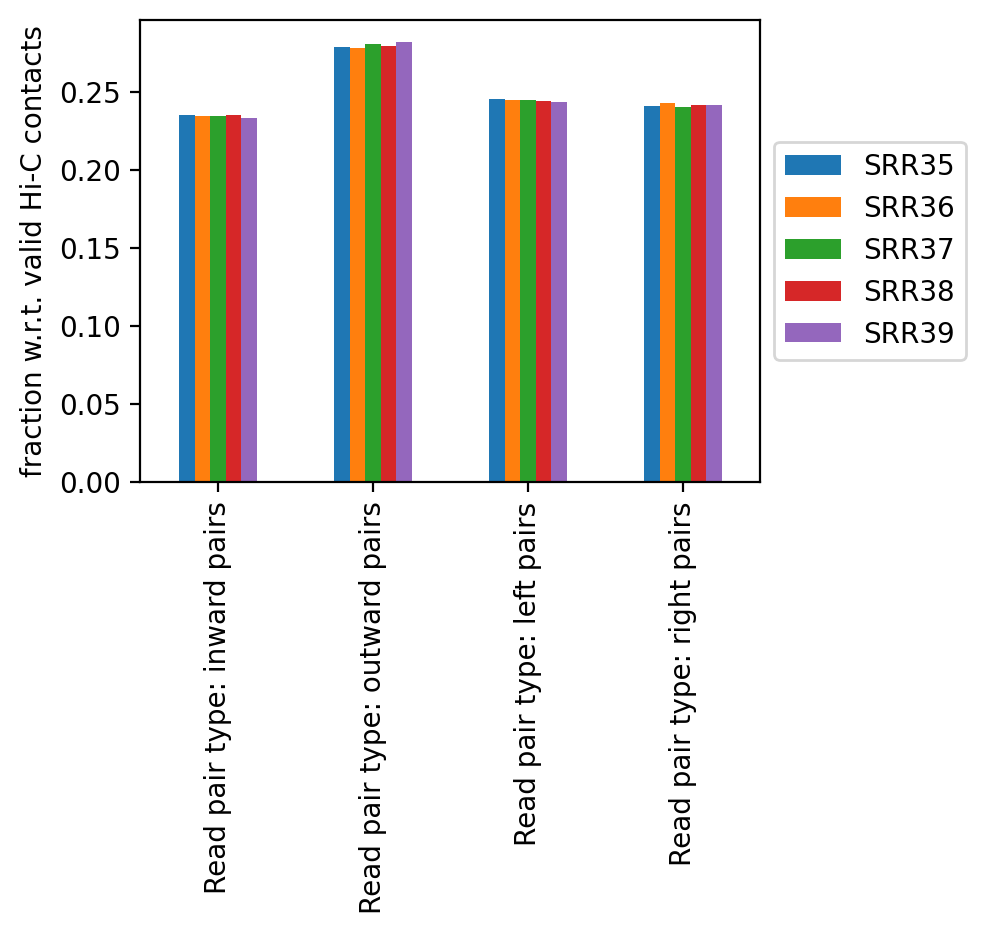
\includegraphics[keepaspectratio]{../steps/bwa/QC_all_samples/read_orientation.png}}

}

\subcaption{\label{fig-explorer-read-orientation}Read orientation}

\end{minipage}%
%
\begin{minipage}{0.33\linewidth}

\centering{

\pandocbounded{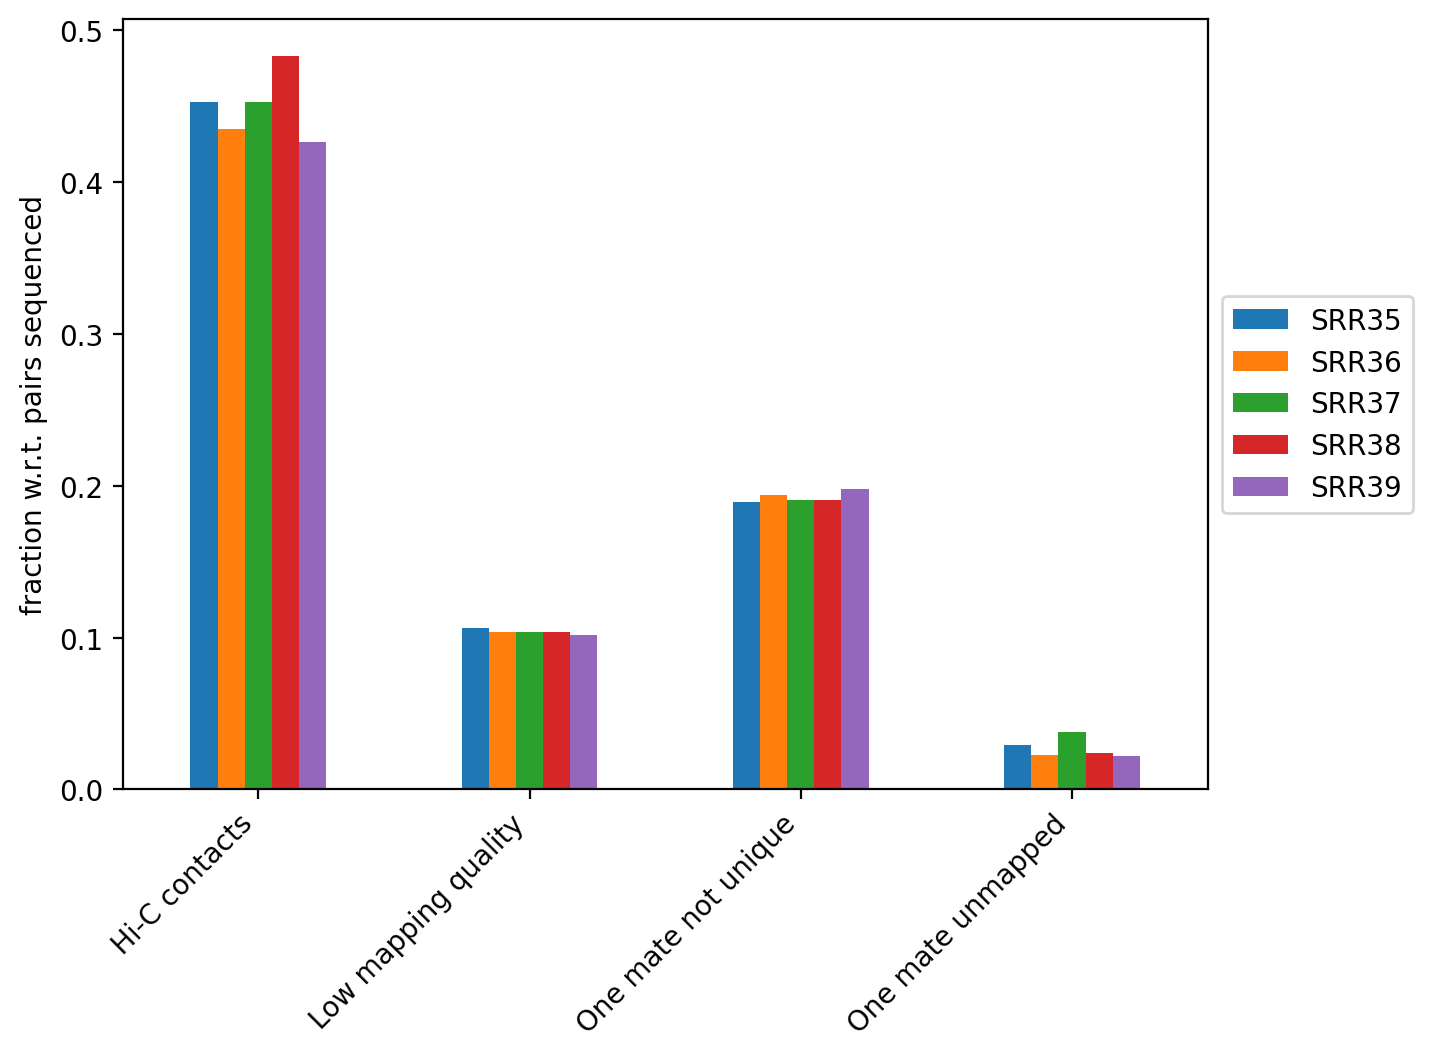
\includegraphics[keepaspectratio]{../steps/bwa/QC_all_samples/unmappable_and_non_unique.png}}

}

\subcaption{\label{fig-explorer-unique-pairs}Unique pairs}

\end{minipage}%
%
\begin{minipage}{0.33\linewidth}

\centering{

\pandocbounded{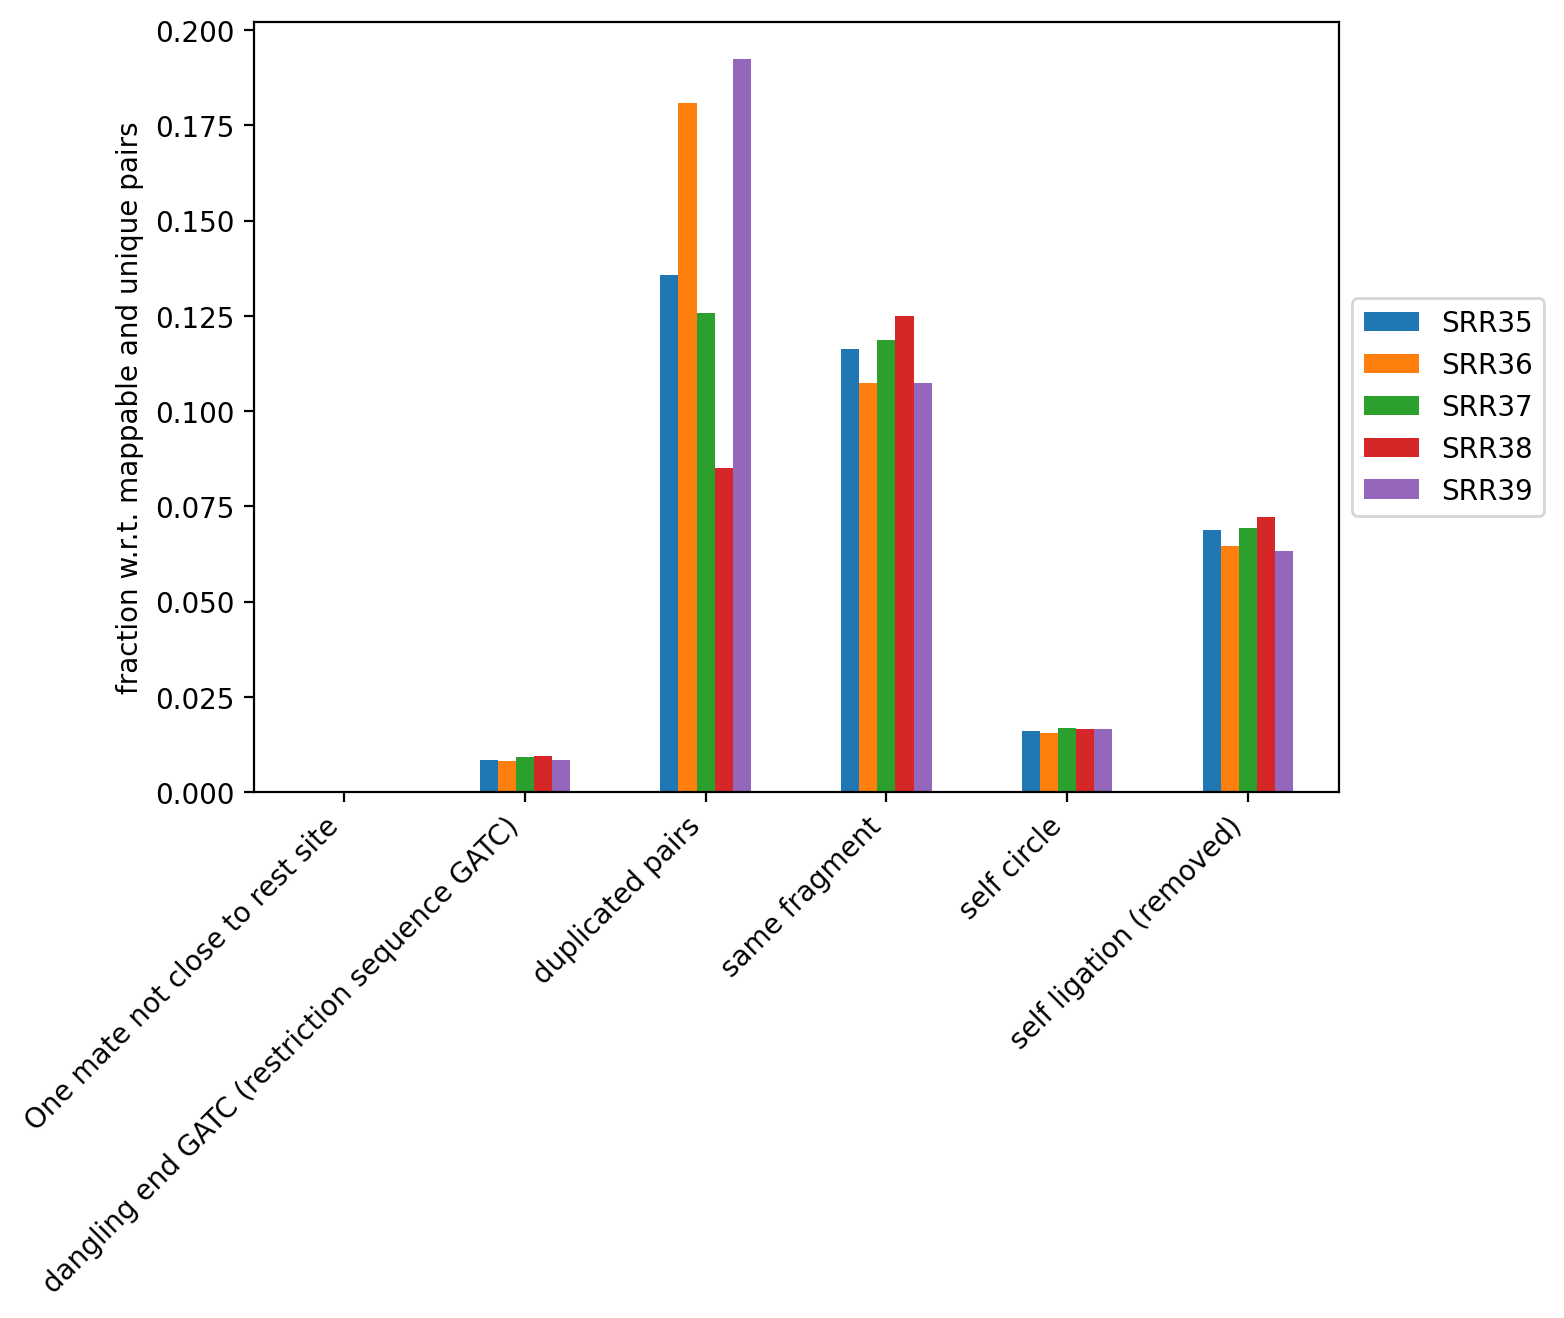
\includegraphics[keepaspectratio]{../steps/bwa/QC_all_samples/pairs_discarded.png}}

}

\subcaption{\label{fig-explorer-discarded-pairs}Discarded pairs}

\end{minipage}%
\newline
\begin{minipage}{0.33\linewidth}

\centering{

\pandocbounded{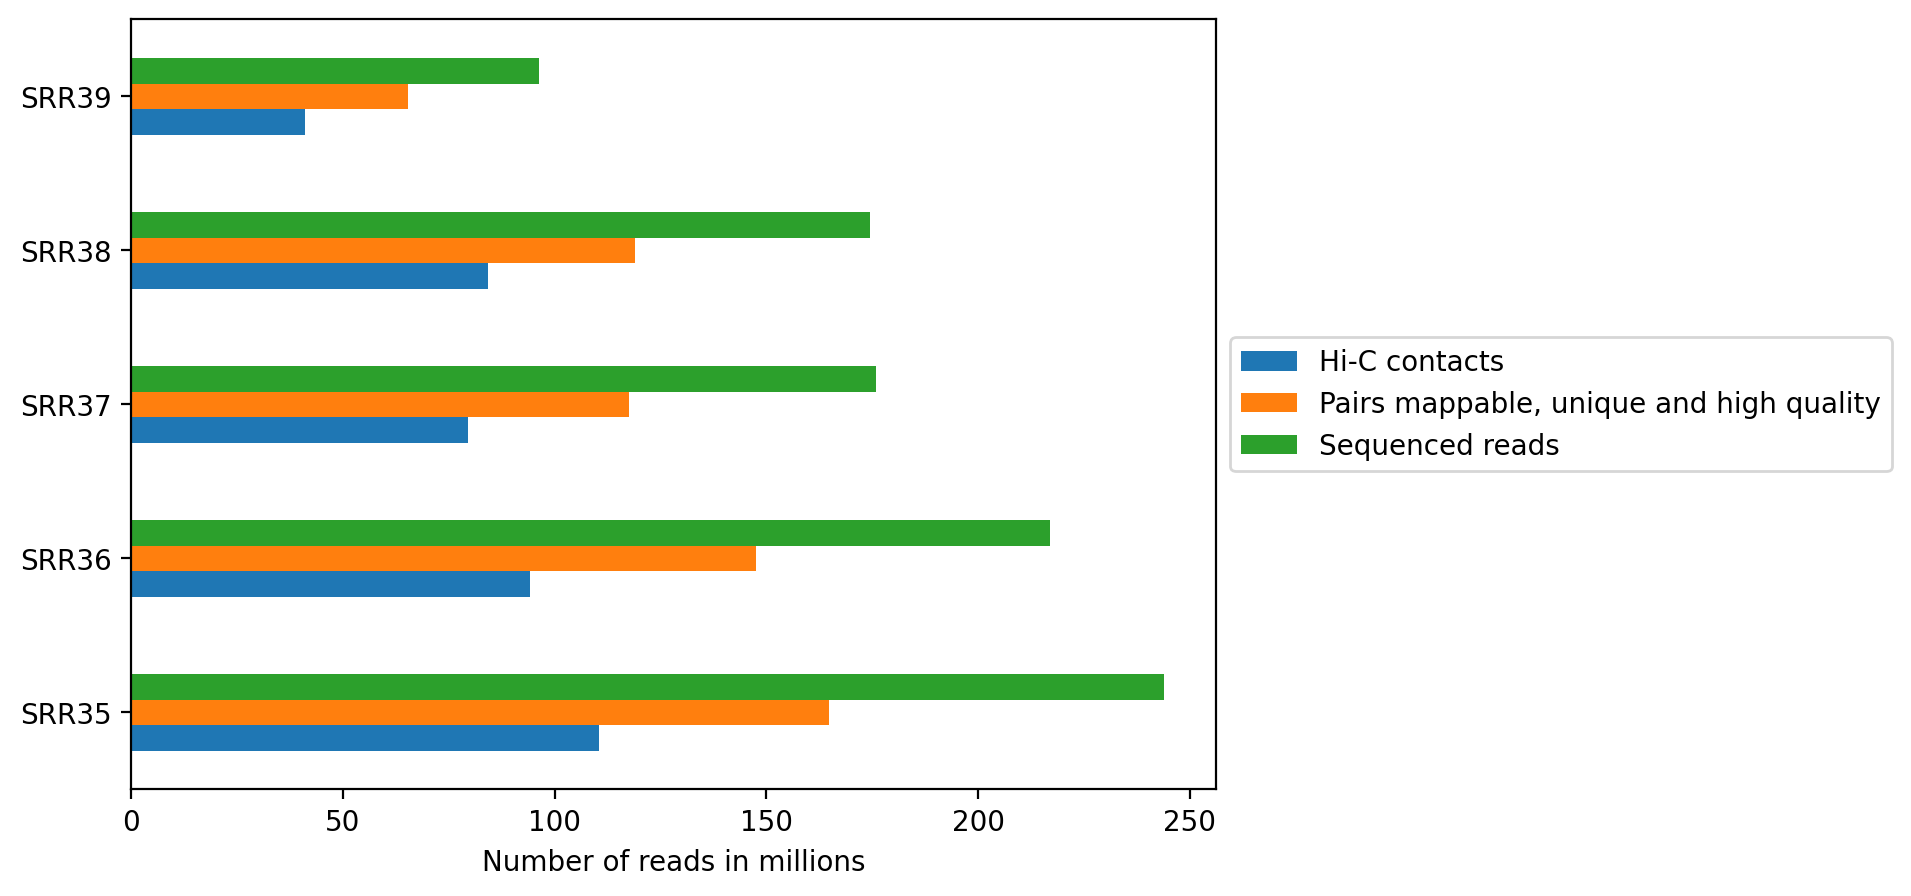
\includegraphics[keepaspectratio]{../steps/bwa/QC_all_samples/pairs_sequenced.png}}

}

\subcaption{\label{fig-explorer-pairs-sequenced}Pairs sequenced}

\end{minipage}%
%
\begin{minipage}{0.33\linewidth}

\centering{

\pandocbounded{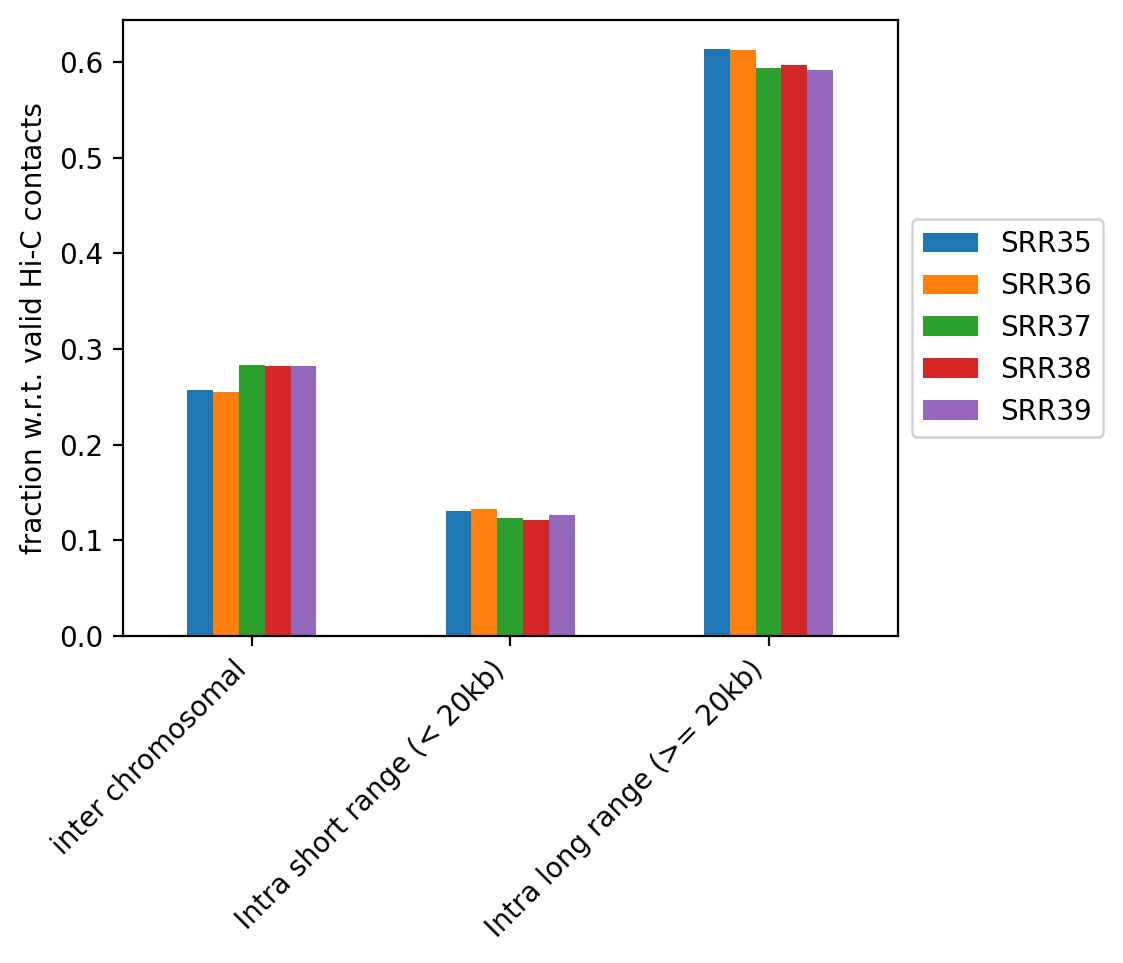
\includegraphics[keepaspectratio]{../steps/bwa/QC_all_samples/distance.png}}

}

\subcaption{\label{fig-explorer-contact-distance}Contact distance}

\end{minipage}%

\caption{\label{fig-explorer-qc}Quality control of the mapped Hi-C reads
using \emph{HiCExplorer} \texttt{hicQC}. The figures should be moved to
Supplementary/Appendix because they are ugly and un-alignable. But that
is the fault of HiCExplorer, not me.}

\end{figure}%

\subsection{Correction}\label{correction}

The correction diagnostic tool yielded a similar \emph{mad} threshold
within the range \([-3,-2]\). Even so, I followed the \emph{HicExplorer}
recommendation to set the lower threshold to at least -2 and the upper
threshold to 5 in the pre-normalization filter. I argue that with a high
number of valid contacts, it is safer to err on the side of caution and
maybe filter out bad data.

\begin{figure}

\begin{minipage}{0.06\linewidth}
~\end{minipage}%
%
\begin{minipage}{0.29\linewidth}

\centering{

\pandocbounded{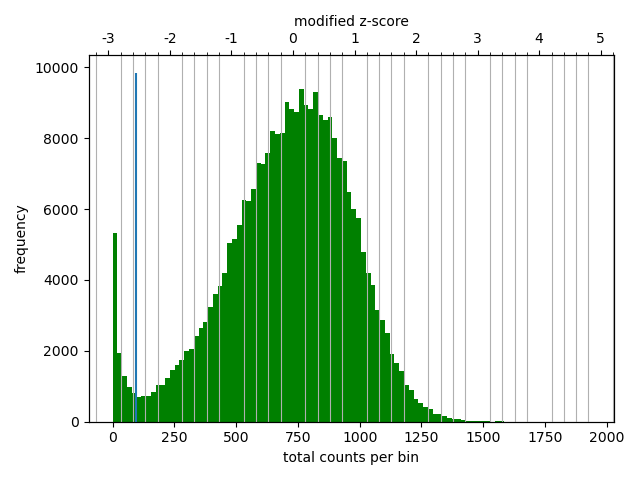
\includegraphics[keepaspectratio]{../figures/bwa/SRR6502335_diag_plot.png}}

}

\subcaption{\label{fig-explorer-pre-correction-SRR6502335}SRR6502335}

\end{minipage}%
%
\begin{minipage}{0.29\linewidth}

\centering{

\pandocbounded{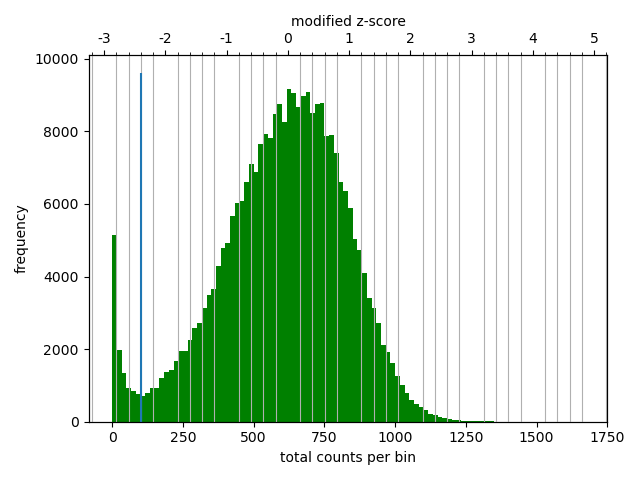
\includegraphics[keepaspectratio]{../figures/bwa/SRR6502336_diag_plot.png}}

}

\subcaption{\label{fig-explorer-pre-correction-SRR6502336}SRR6502336}

\end{minipage}%
%
\begin{minipage}{0.29\linewidth}

\centering{

\pandocbounded{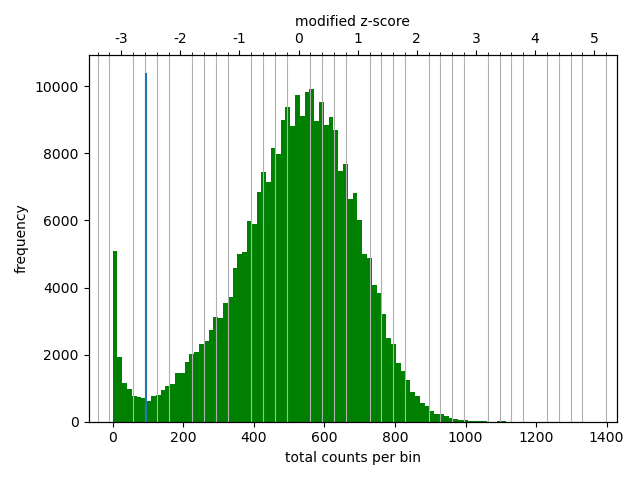
\includegraphics[keepaspectratio]{../figures/bwa/SRR6502337_diag_plot.png}}

}

\subcaption{\label{fig-explorer-pre-correction-SRR6502337}SRR6502337}

\end{minipage}%
%
\begin{minipage}{0.06\linewidth}
~\end{minipage}%
\newline
\begin{minipage}{0.21\linewidth}
~\end{minipage}%
%
\begin{minipage}{0.29\linewidth}

\centering{

\pandocbounded{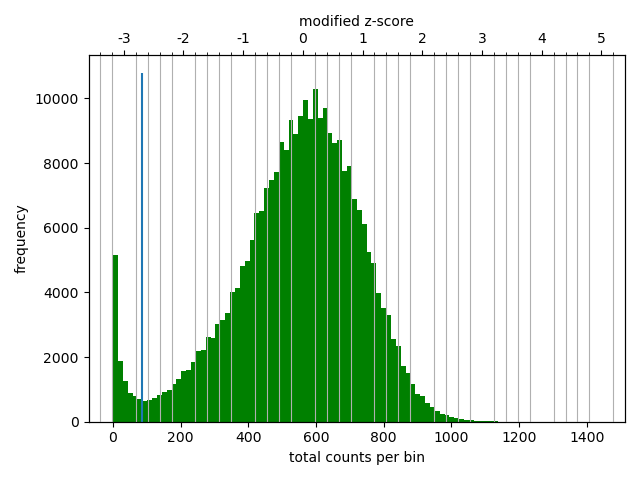
\includegraphics[keepaspectratio]{../figures/bwa/SRR6502338_diag_plot.png}}

}

\subcaption{\label{fig-explorer-pre-correction-SRR6502338}SRR6502338}

\end{minipage}%
%
\begin{minipage}{0.29\linewidth}

\centering{

\pandocbounded{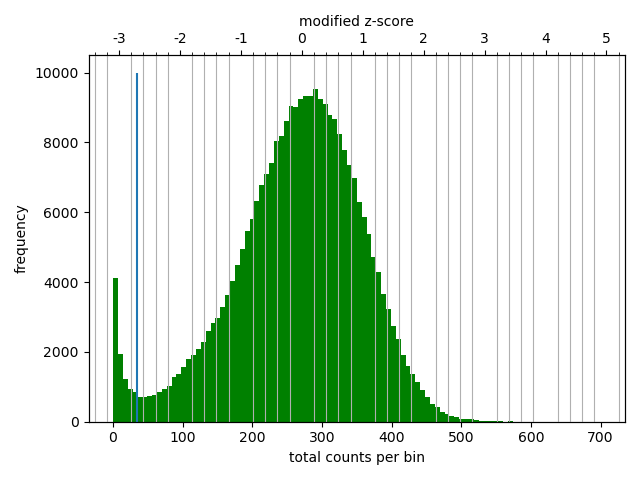
\includegraphics[keepaspectratio]{../figures/bwa/SRR6502339_diag_plot.png}}

}

\subcaption{\label{fig-explorer-pre-correction-SRR6502339}SRR6502339}

\end{minipage}%
%
\begin{minipage}{0.21\linewidth}
~\end{minipage}%

\caption{\label{fig-explorer-pre-correction}Histograms of the number of
counts per bin (bottom x-axis) and the modified z-score (top x-axis)
from which the \emph{mad} threshold is defined.}

\end{figure}%

To compare these mappings with others, the QC results is an easy way.
Therefore, the reads were mapped with \emph{bowtie2} in both end-to-end-
and local-mode followed by \texttt{hiCBuildMatrix}, and the QC from each
method was plotted next to each other
(Figure~\ref{fig-explorer-all-3-qc}). Interestingly, \emph{bowtie2} was
much more computer-intensive in both modes, perhaps because of the
\texttt{-\/-very-sensitive} option. In any case, the QC reveals a major
difference in the total number of reads that are determined to be valid
Hi-C contacts by \texttt{hicBuildMatrix}. As expected, mapping with
\emph{end-to-end-bowtie2} makes locating Hi-C contacts more difficult
than the other methods (Figure~\ref{fig-explorer-all-3-qc}, top row),
finding a very low amount of mappable, unique pairs passing the quality
threshold. In contrast, mapping with \emph{local-bowtie2} performs
similarly to \emph{bwa} in finding mappable, unique, high-quality pairs,
but calls only approximately half the number of valid Hi-C contacts
(\textgreater20\%), resulting in a fraction of valid Hi-C pairs that
hits the expectation from \emph{HicExplorer} docs {[}ref row3{]}. With
\emph{bwa}, the reads were discarded either due to low mapping quality
or non-unique mates, whereas with \emph{local-bowtie2}, the reads were
almost exclusively filtered out due to low mapping quality. This must be
a result of how the mappers assign mapping quality, and I believe
\emph{local-bowtie2} looks suspiciously selective in finding unique but
low quality alignments. \emph{end-to-end-bowtie} almost exclusively
filters out read-pairs where one mate is unmapped, which is expected
when the majority of reads are unmapped.

\begin{figure}[H]

\centering{

\pandocbounded{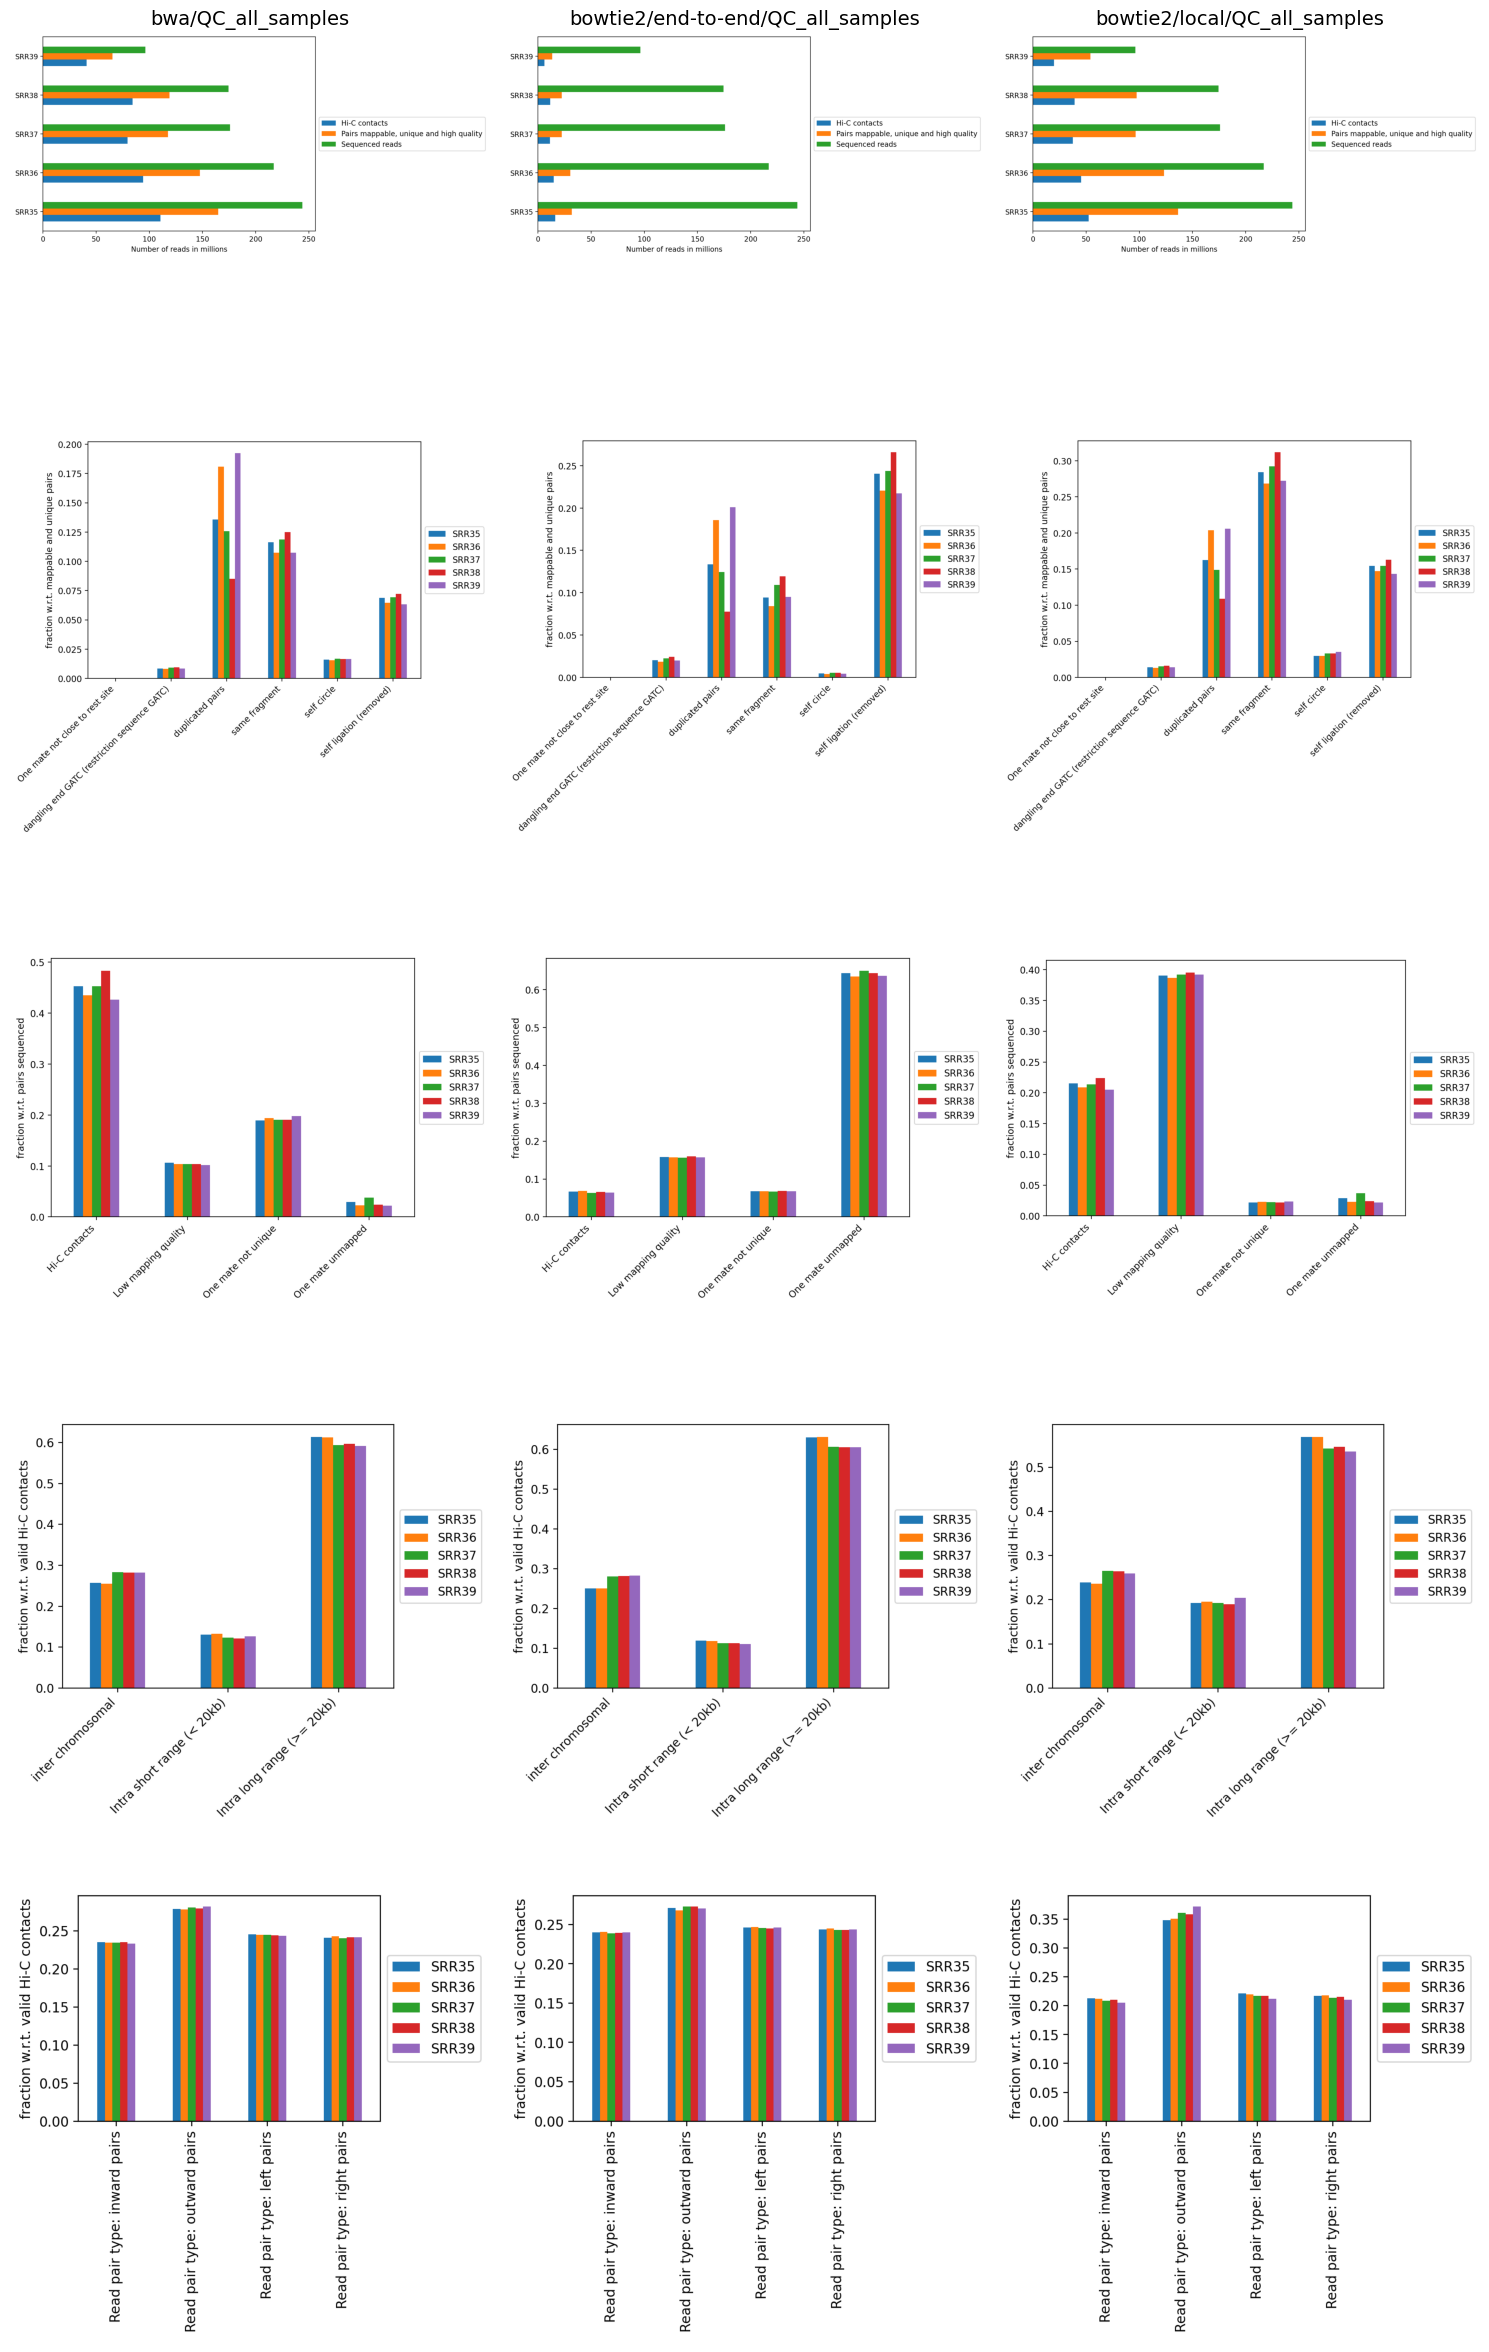
\includegraphics[keepaspectratio]{index_files/figure-latex/..-notebooks-01_hicexplorer-fig-explorer-all-3-qc-output-1.png}}

}

\caption{\label{fig-explorer-all-3-qc}Comparison of HiCExplorer QC plots
for all samples using different alignment tools.}

\end{figure}%

As discussed, the five samples were pooled with \texttt{hicSumMatrices},
and the non-standard contigs (unplaced scaffolds) were filtered out, and
the different resolutions were created (\texttt{hicMergeMatrixBins}).
\emph{HiCExplorer} also comes with a normalization function prior to
correcting the matrix, which should be applied if different samples
should have comparable bin counts. It has no effect when having only one
matrix. Nevertheless, the pooled matrix was normalized and then
corrected compared in Figure~\ref{fig-explorer-pooled-norm-normcorr}.

\begin{figure}

\begin{minipage}{0.50\linewidth}

\centering{

\pandocbounded{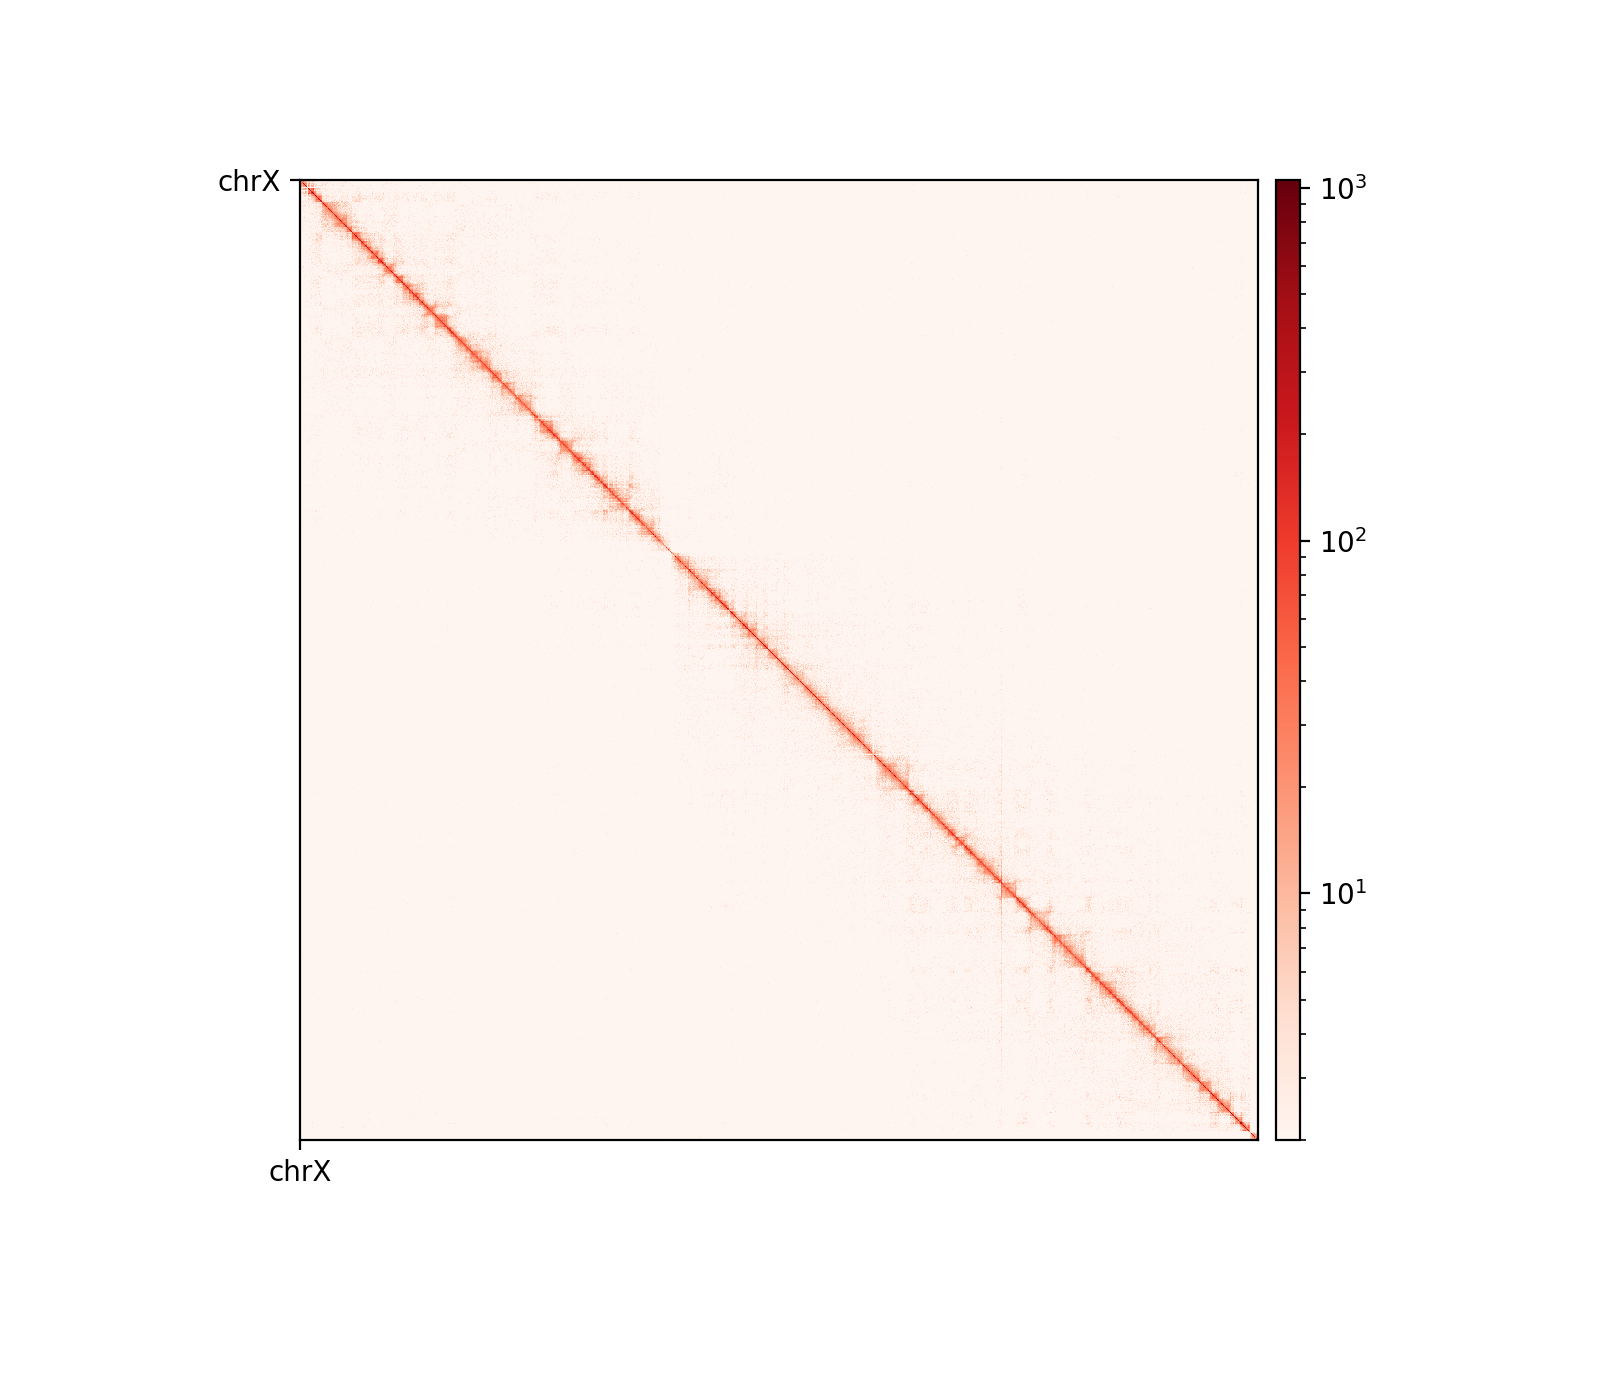
\includegraphics[keepaspectratio]{../figures/bowtie2/local/filter_pooled_50kb_chrX.png}}

}

\subcaption{\label{fig-explorer-pooled-chrX-norm}Normalized matrix chrX}

\end{minipage}%
%
\begin{minipage}{0.50\linewidth}

\centering{

\pandocbounded{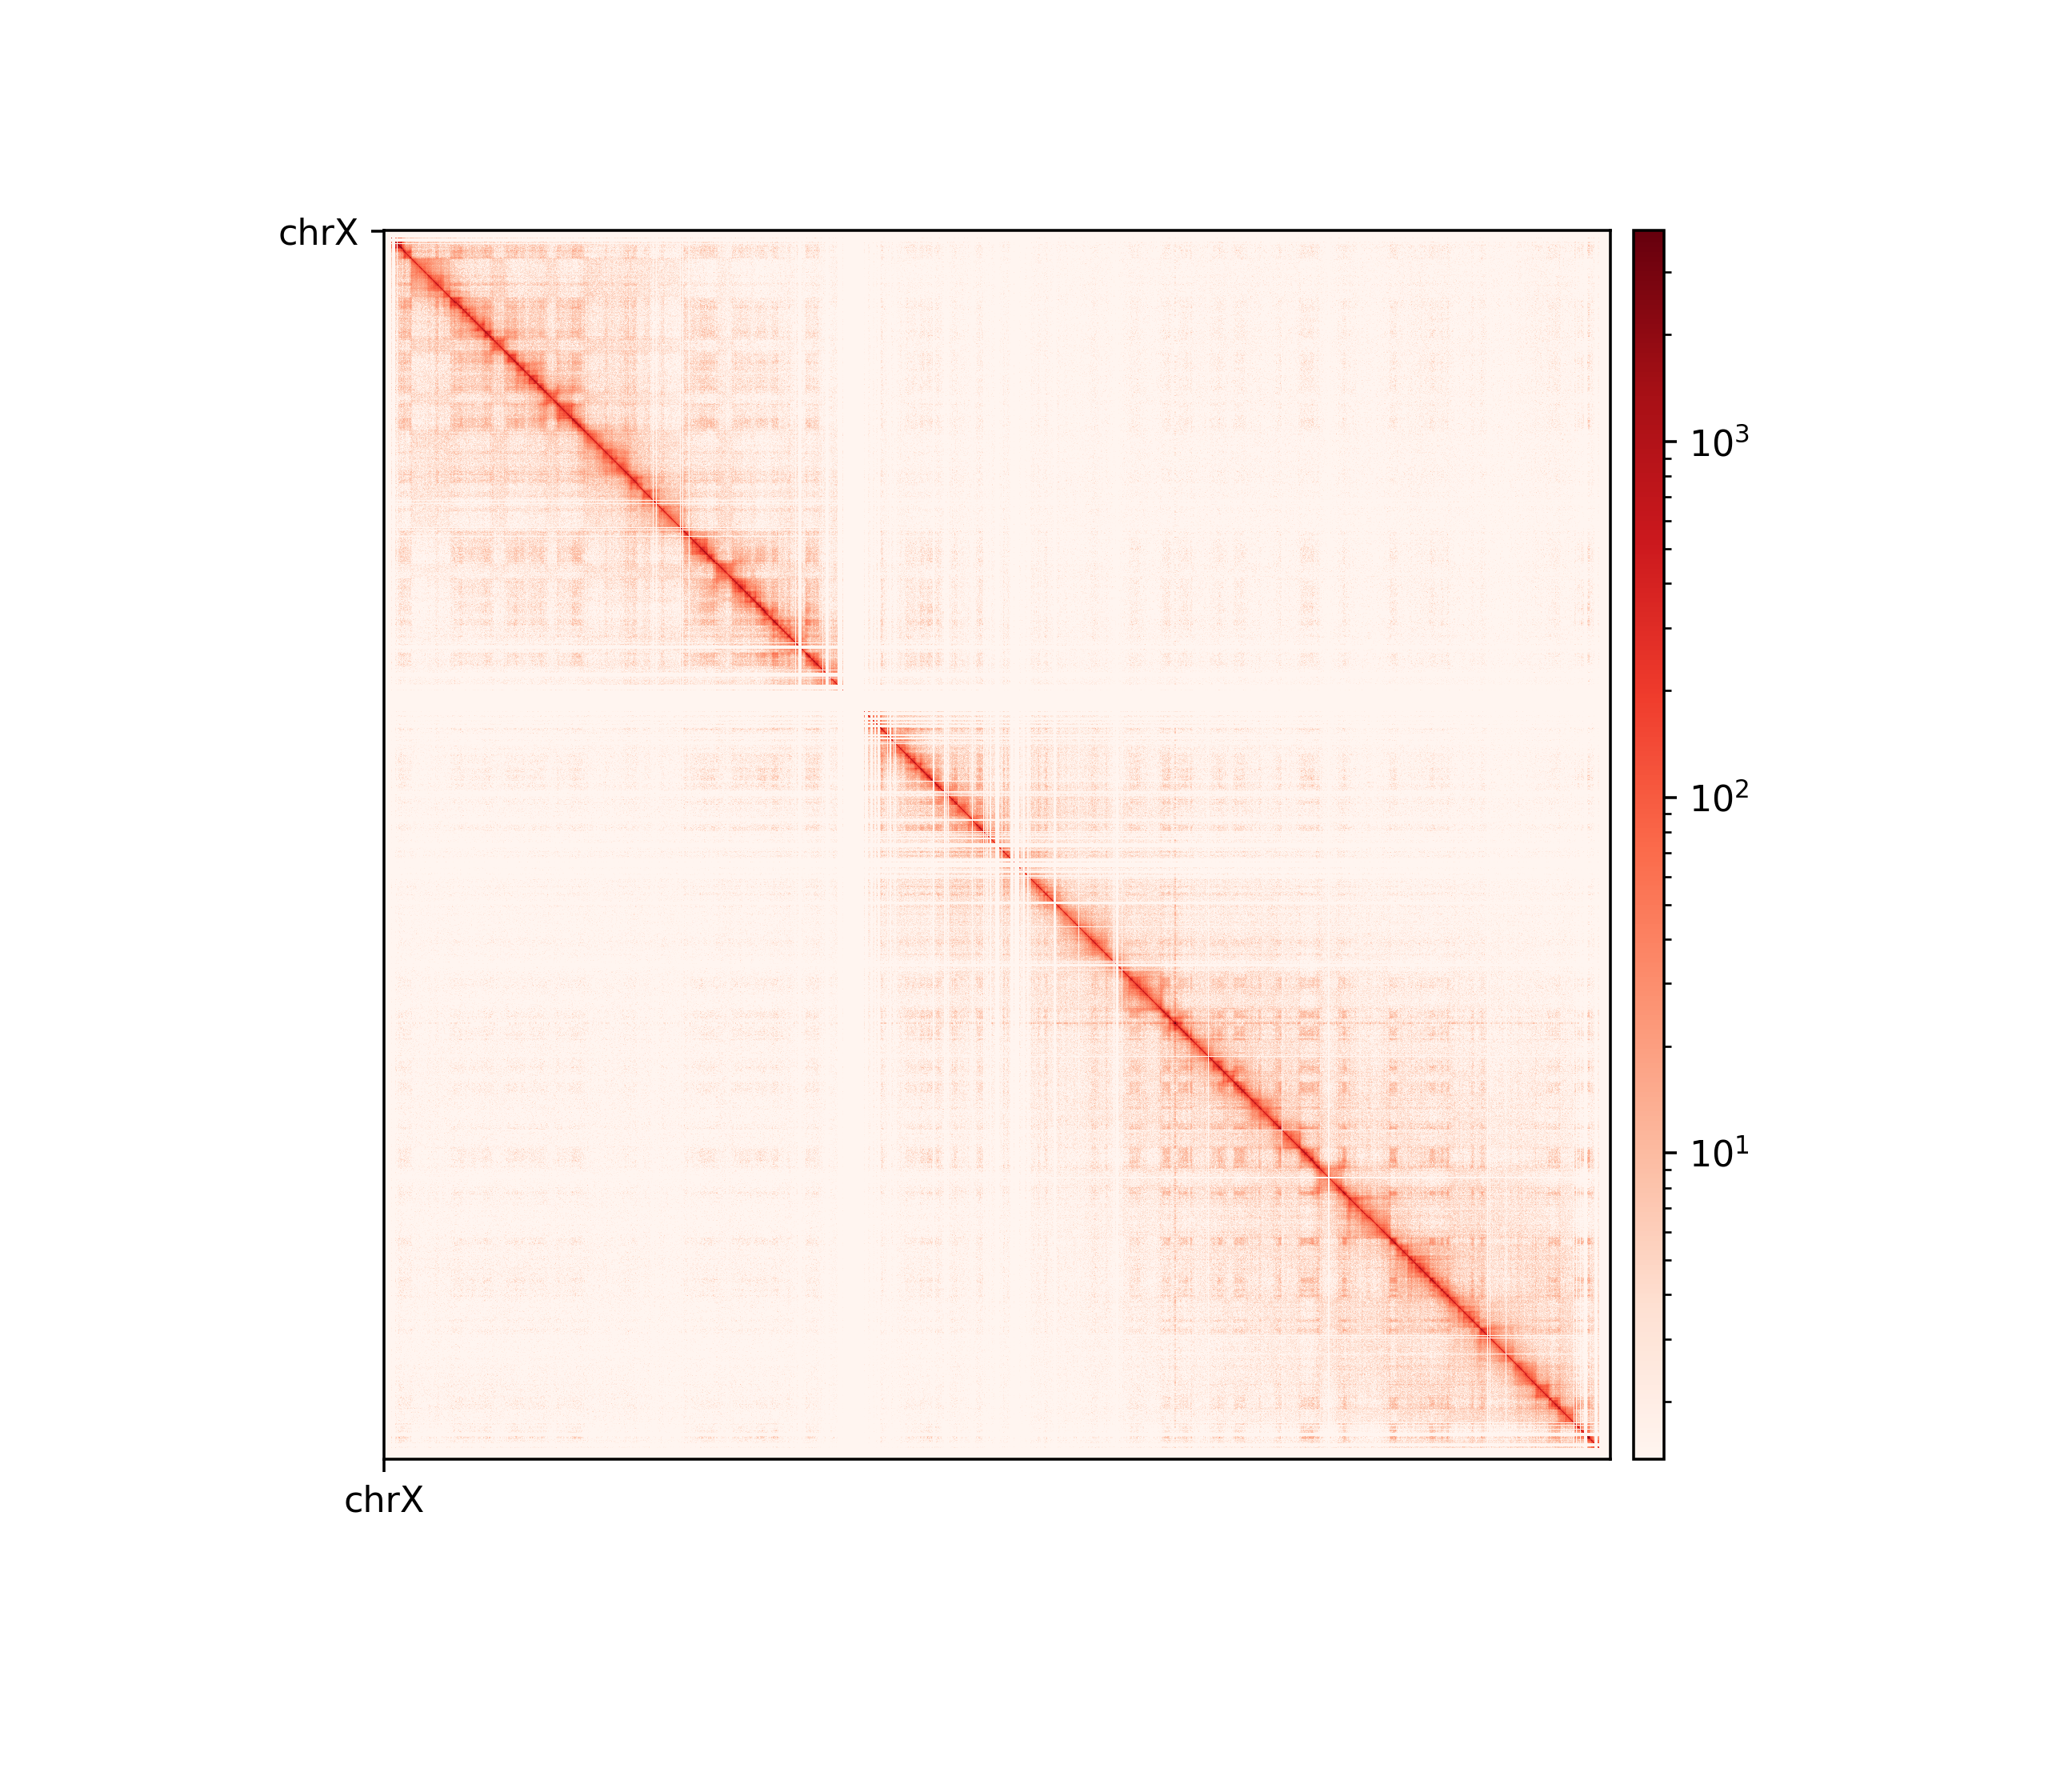
\includegraphics[keepaspectratio]{../figures/bowtie2/local/normalized/normsm_filter_pooled_100kb_corrected_chrX-full.png}}

}

\subcaption{\label{fig-explorer-pooled-chrX-normcorr}Normalized and
corrected chrX}

\end{minipage}%

\caption{\label{fig-explorer-pooled-norm-normcorr}A comparison of
interaction matrices before/after iterative correction
(\emph{HiCExplorer}).}

\end{figure}%

It is now obvious why we have to correct the matrix. The uncorrected
(Figure~\ref{fig-explorer-pooled-chrX-norm}) has no signal apart from
the diagonal. Even though some bins have been filtered out, the expected
\emph{plaid} pattern of a contact matrix is visible along the diagonal
after the correction (Figure~\ref{fig-explorer-pooled-chrX-normcorr}),
leaving evidence for chromatin structure, especially in the first 50
million bases of the chromosome. There is a wide region of empty values
at the place of the centromere.

\subsection{Eigenvectors}\label{eigenvectors}

The PCA performed by \texttt{hicPCA} on the pooled samples at both 50kb
and 100kb resolution yielded the first 3 principal components. For PC1
on both resolutions (Figure~\ref{fig-explorer-pc1-50kb},
Figure~\ref{fig-explorer-pc1-100kb}) we observe only a single sign
change which occurs at around 60 Mbp, the region of the centromere. It
means the PCA has captured more variance between the chromosome arms
than within them, making it uninformative about chromatin compartments.
Upon visual inspection, it is clear that neither of the PC graphs
capture the pattern of the interaction matrix by its change of sign. It
seems the PCs capture variance from a bias that varies slowly and
predictably along the chromosome. The first PC that is supposed to
capture the compartments very suspiciously changes sign at the region of
the centromere, a classic problem that could be solved by restricting
the values from which the PC is calculated along the chromosome.
Unimpressed, I rationalize that the option \texttt{-\/-extra-track} to
provide a gene track or histone coverage should not affect this result
much. It should be provided as a phasing track to orient the eigenvector
to positively correlate with gene density or histone marks, and could
possibly muddle the compartments if not included. I followed
\emph{HiCExplorer} pipeline to plot and explore the matrices. At this
point, I stoppped using \emph{HiCExplorer}, as I assessed that a more
flexible tool was needed.

\begin{figure}

\begin{minipage}{0.33\linewidth}

\centering{

\pandocbounded{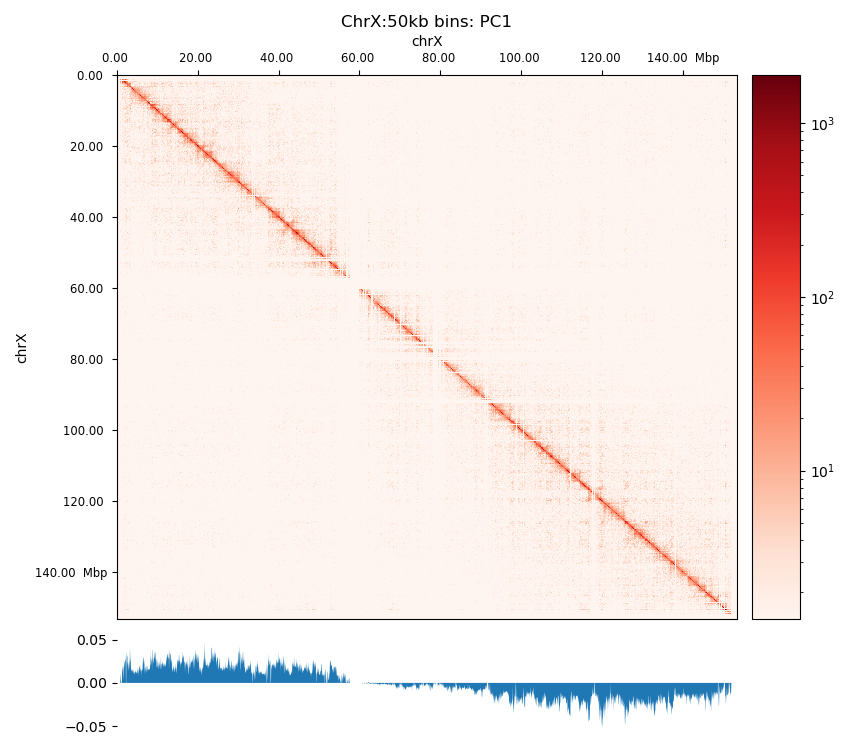
\includegraphics[keepaspectratio]{../figures/bowtie2/local/normalized/pc1_50kb_corrected_chrX.png}}

}

\subcaption{\label{fig-explorer-pc1-50kb}}

\end{minipage}%
%
\begin{minipage}{0.33\linewidth}

\centering{

\pandocbounded{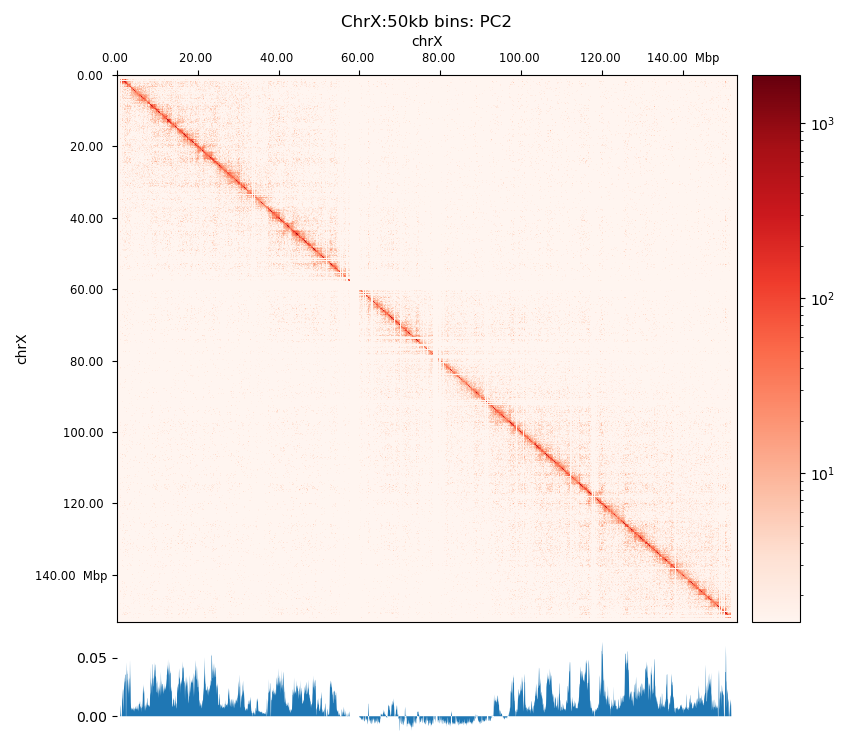
\includegraphics[keepaspectratio]{../figures/bowtie2/local/normalized/pc2_50kb_corrected_chrX.png}}

}

\subcaption{\label{fig-explorer-pc2-50kb}}

\end{minipage}%
%
\begin{minipage}{0.33\linewidth}
\pandocbounded{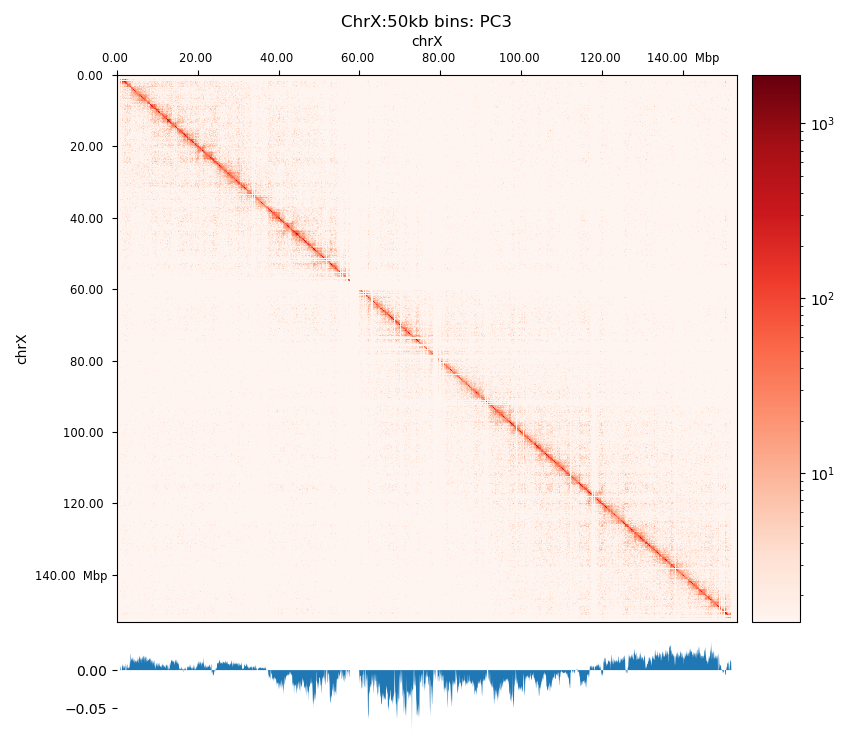
\includegraphics[keepaspectratio]{../figures/bowtie2/local/normalized/pc3_50kb_corrected_chrX.png}}\end{minipage}%
\newline
\begin{minipage}{0.33\linewidth}

\centering{

\pandocbounded{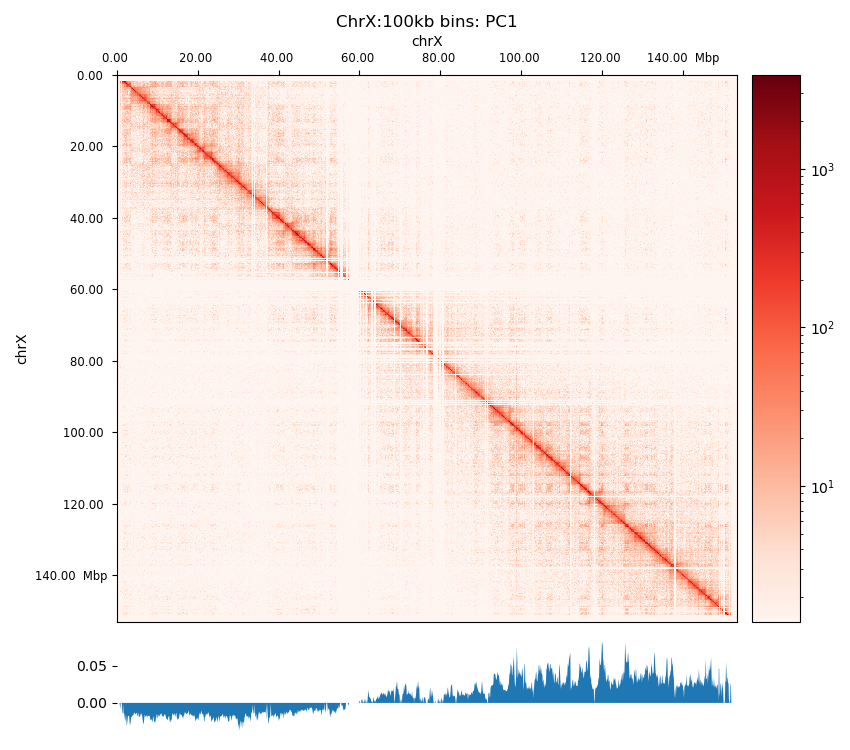
\includegraphics[keepaspectratio]{../figures/bowtie2/local/normalized/pc1_100kb_corrected_chrX.png}}

}

\subcaption{\label{fig-explorer-pc1-100kb}}

\end{minipage}%
%
\begin{minipage}{0.33\linewidth}

\centering{

\pandocbounded{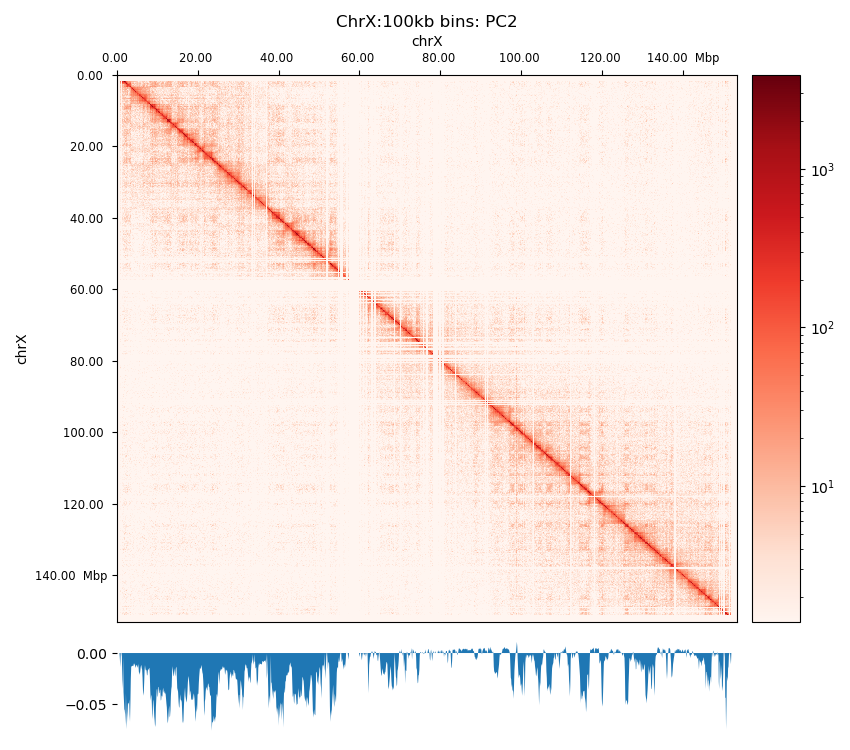
\includegraphics[keepaspectratio]{../figures/bowtie2/local/normalized/pc2_100kb_corrected_chrX.png}}

}

\subcaption{\label{fig-explorer-pc2-100kb}}

\end{minipage}%
%
\begin{minipage}{0.33\linewidth}

\centering{

\pandocbounded{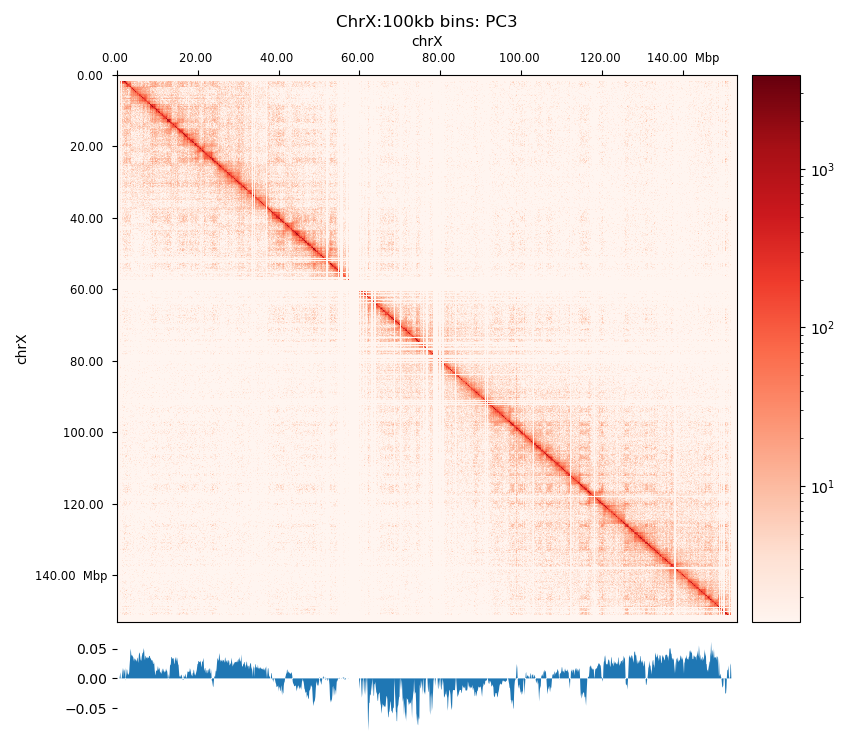
\includegraphics[keepaspectratio]{../figures/bowtie2/local/normalized/pc3_100kb_corrected_chrX.png}}

}

\subcaption{\label{fig-explorer-pc3-100kb}}

\end{minipage}%

\caption{\label{fig-explorer-pca}Corrected interaction matrix for
chromosome X along with PC1, 2, or 3, respectively. a-c: 50kb
resolution, d-f: 100kb resolution. \emph{HiCExplorer}.}

\end{figure}%

\section{Open2c ecosystem}\label{open2c-ecosystem}

\subsection{Quality Control}\label{quality-control-1}

As described, the pairtools module in MultiQC (Ewels et al. 2016) was
used to visualize results from \texttt{pairtools\ stats} for the two
parsing runs, see Figure~\ref{fig-pairtools-qc}.

\subsubsection{\texorpdfstring{\texttt{-\/-walks-policy\ mask}}{-\/-walks-policy mask}}\label{walks-policy-mask}

Comparing the multiQC report for each of the cell sources show similar
distributions of \emph{unmapped} (both sides unmapped), \emph{one-sided}
(one side mapped), \emph{two-sided} (both sides mapped), and
\emph{duplicated} (w.r.t. total mapped) reads. The percentage of
\emph{cis} pairs w.r.t. mapped pairs is around 70\% for all samples
(Figure~\ref{fig-pairtools-multiqc-mask-violin}). The valid pairs also
show similar distributions of pair types divided into 10 categories. The
\(P(s)\) curve looks similar for all samples as well, peaking around 250
bp separation (Figure~\ref{fig-pairtools-multiqc-mask-ps}). The QC does
not show any information about mapping quality of the reads. Note that
the \(P(s)\) curve arise from pre-filtered pairs, meaning it provides
information about the Hi-C library. As expected

\subsubsection{\texorpdfstring{\texttt{-\/-walks-policy\ 5unique}}{-\/-walks-policy 5unique}}\label{walks-policy-5unique}

Parsing alignments with the recommended walks-policy aproximately halves
the percentage of \emph{unmapped} reads, and \emph{one-} and
\emph{two-sided} reads as well \emph{duplicated} reads are slightly
increased. Overall number of unique pairs are increased with more than
20\% increase. The percentage of \emph{cis} pairs are only decreased by
a percentage point at most
(Figure~\ref{fig-pairtools-multiqc-5unique-violin}). Changing the walks
policy does not alter the \(P(s)\) curve, meaning the parameter does not
bias the parsing w.r.t. genomic separation.

\begin{figure}

\begin{minipage}{0.50\linewidth}

\centering{

\pandocbounded{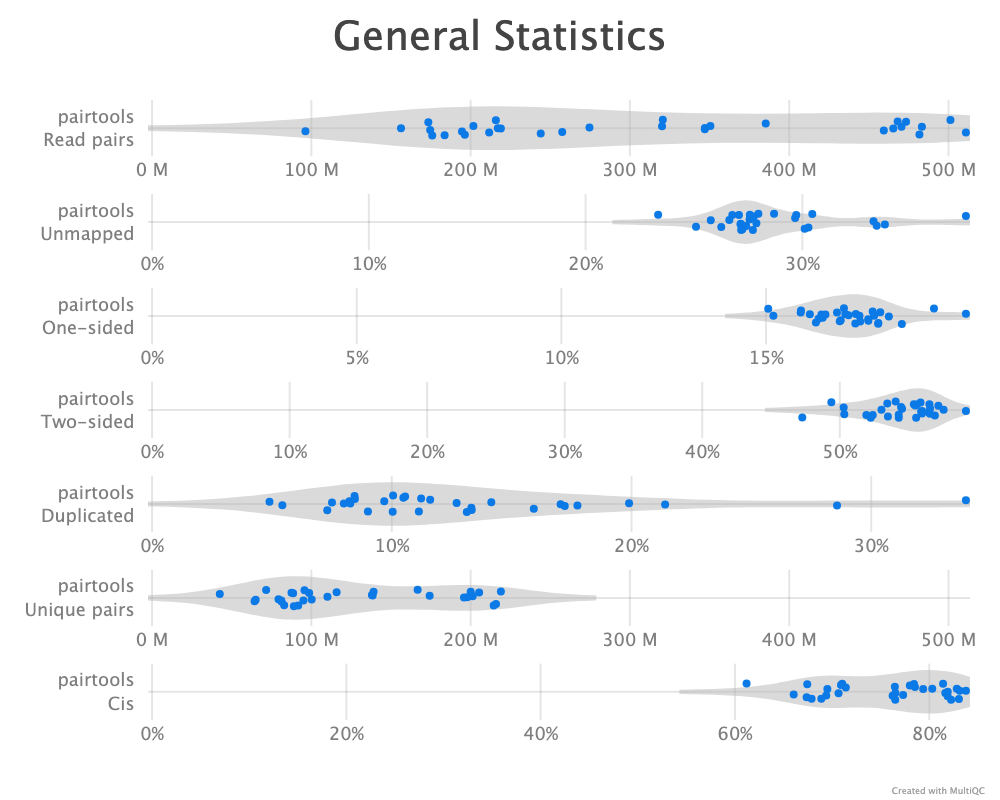
\includegraphics[keepaspectratio]{../figures/fig-pairtools-parse-multiqc-mask-violin.png}}

}

\subcaption{\label{fig-pairtools-multiqc-mask-violin}\texttt{-\/-walks-policy\ mask}}

\end{minipage}%
%
\begin{minipage}{0.50\linewidth}

\centering{

\pandocbounded{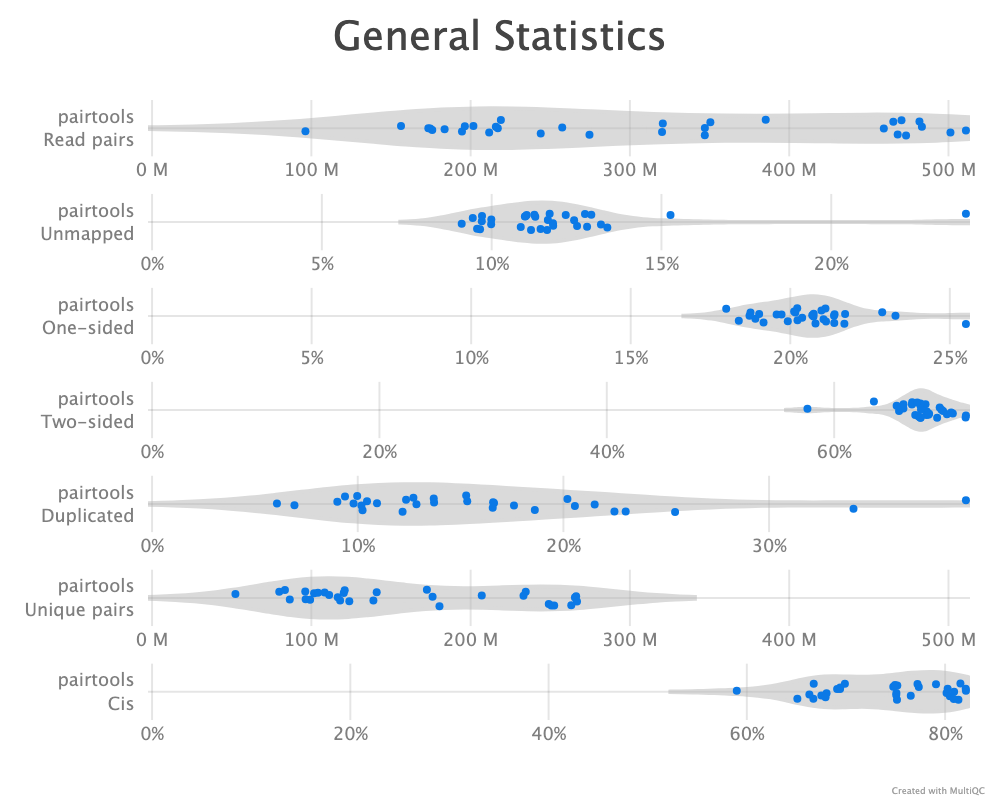
\includegraphics[keepaspectratio]{../figures/fig-pairtools-parse-multiqc-5unique-violin.png}}

}

\subcaption{\label{fig-pairtools-multiqc-5unique-violin}\texttt{-\/-walks-policy\ 5unique}}

\end{minipage}%
\newline
\begin{minipage}{0.50\linewidth}

\centering{

\pandocbounded{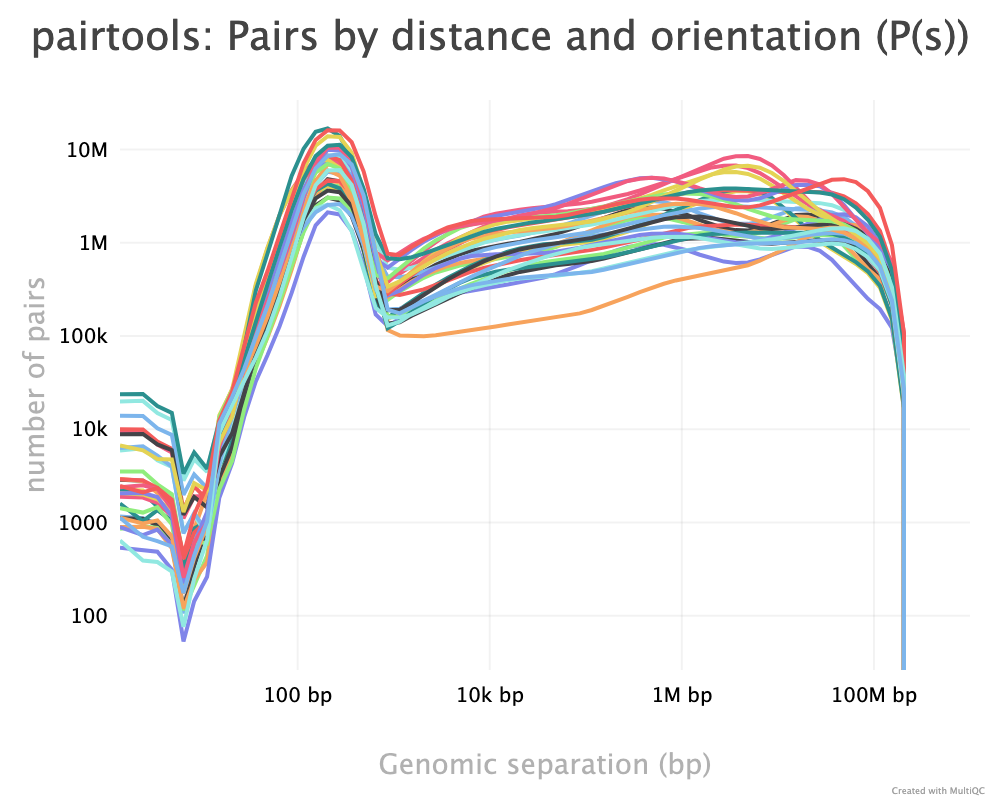
\includegraphics[keepaspectratio]{../figures/fig-pairtools-parse-multiqc-mask-ps.png}}

}

\subcaption{\label{fig-pairtools-multiqc-mask-ps}\texttt{-\/-walks-policy\ mask}}

\end{minipage}%
%
\begin{minipage}{0.50\linewidth}

\centering{

\pandocbounded{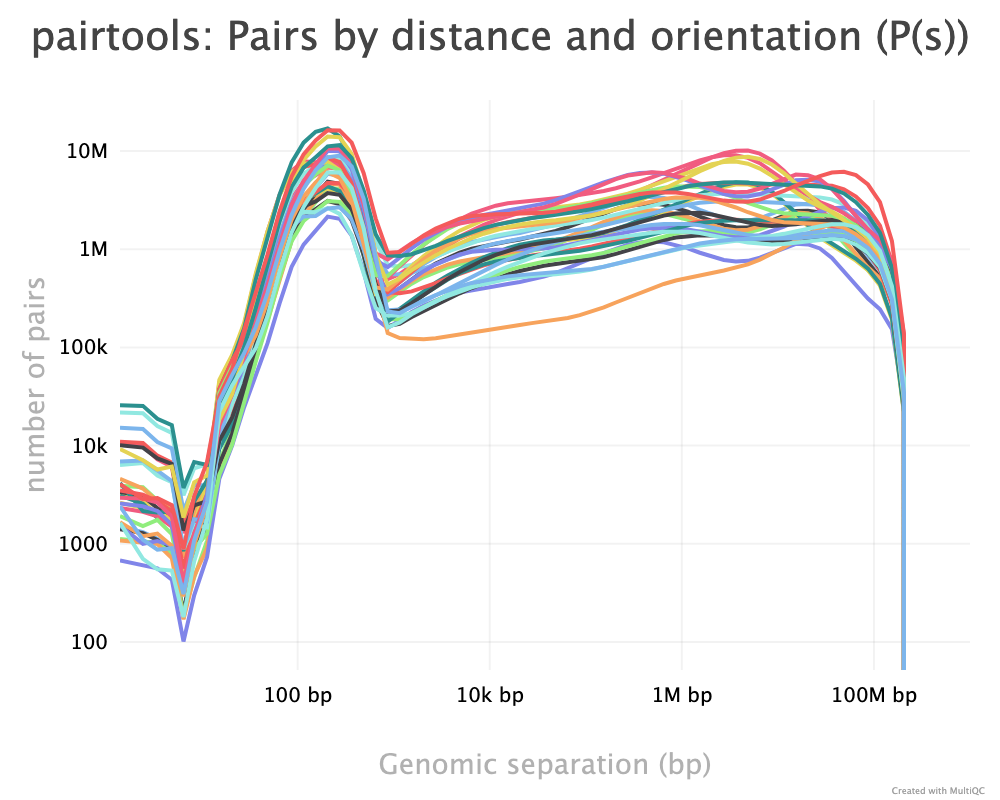
\includegraphics[keepaspectratio]{../figures/fig-pairtools-parse-multiqc-5unique-ps.png}}

}

\subcaption{\label{fig-pairtools-multiqc-5unique-ps}\texttt{-\/-walks-policy\ 5unique}}

\end{minipage}%

\caption{\label{fig-pairtools-qc}Results of \texttt{pairtools\ stats}
run on all samples from the two walks-policies. Left (a+c):
\texttt{mask}; right (b+d): \texttt{5unique}. \emph{Generated by
MultiQC} (Ewels et al. 2016). \emph{Note: X-axes are not shared in the
`Genereal Statistics' plot.}}

\end{figure}%

\subsection{Correction}\label{correction-1}

Matrix balancing did not show major improvement in the plaid pattern, as
it already showed the expected pattern. It does, however, filter out
bins that are deemed too low-count to be informative, for example
peri-centromeric regions. The matrix was expected to be smoother after
balancing (for chromosome-wide maps), as regions along a chromosome
should only vary slowly in contact frequency with other regions as they
are on a continouos molecule. Therefore, sharp contrasts represent a
sudden drop in bin count (Figure~\ref{fig-rs-chrx-raw-balanced-cgi},
raw) and should not be interpreted as devoid of interaction, but an
indication that the data is not sufficient to interpret. It is then
better to simply remove the bins in stead of correcting, which will also
amplify noise. Even with a high-quality Hi-C library we expect that all
bins do not have the same coverage throughout(Lajoie, Dekker, and Kaplan
2015), as restriction enzymes do not bind equally to all regions of the
genome, and therefore, some bins will be underrepresented as an artefact
of binding/cutting efficieny of the restriction enzyme used.

\begin{figure}[H]

\centering{

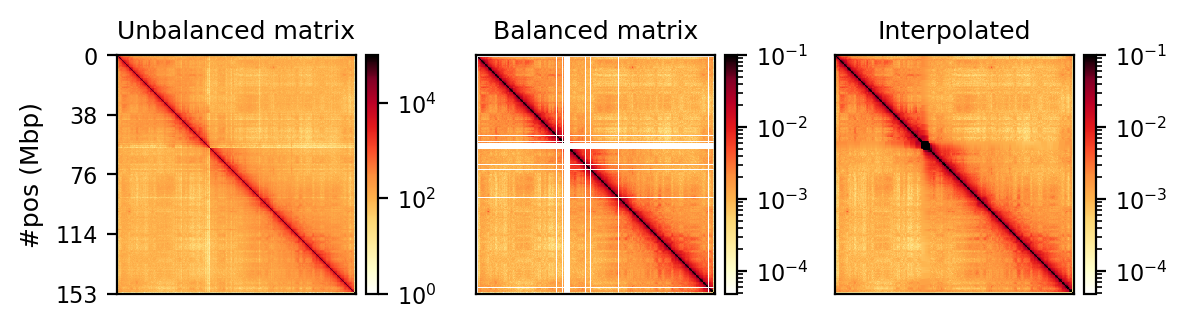
\includegraphics[width=6.17708in,height=1.70833in]{index_files/figure-latex/..-notebooks-05_rec_compartments-fig-rs-chrx-raw-balanced-cgi-output-2.png}

}

\caption{\label{fig-rs-chrx-raw-balanced-cgi}Raw, balanced, and
interpolated chrX interaction matrix in 500kb resolution. The
interpolation is done to make the matrix more visually appealing, but it
is not necessary for the analysis.}

\end{figure}%

\begin{figure}[H]

\centering{

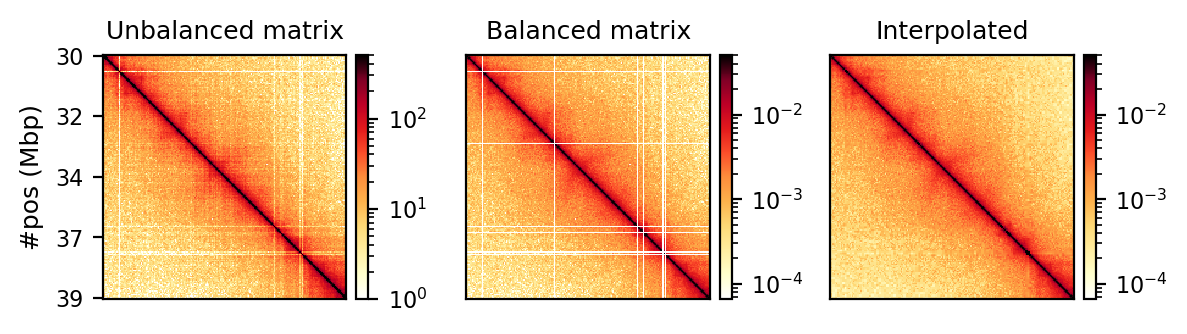
\includegraphics[width=6.17708in,height=1.73958in]{index_files/figure-latex/..-notebooks-05_rec_compartments-fig-rs-chrx-raw-balanced-cgi-subset-output-2.png}

}

\caption{\label{fig-rs-chrx-raw-balanced-cgi-subset}Raw, balanced, and
interpolated chrX interaction matrix in 50kb resolution. The
interpolation is done to make the matrix more visually appealing, but it
is not necessary for the analysis.}

\end{figure}%

We can try to mitigate the white lines of empty bins that now appear in
the matrices. The coarsegrained and interpolated matrix is useful to
make a good-looking interaction matrix, but is not that useful for
analysis purposes. It might get easier to visually inspect the matrix,
but it is not clear how well the interpolated matrix reflects the
structure of the chromatin, and it is not transparent which regions are
interpolated and which that are not. I find it purposeful for
interpolation on high-resolution (zoomed-in) views
(Figure~\ref{fig-rs-chrx-raw-balanced-cgi-subset}) with small empty
regions, but misleading for chromosome-wide maps, where typically the
centromere and extremities of the chromosome have filtered-out bins.
Interpolation is further discussed below.

The regions that are coarsgrained are small zero- or low-count bins
which are averaged, effectively reducing the resolution of those regions
until the count is sufficient. They get more frequent the longer genomic
distance (the further we travel from the diagonal), and effectively
enables us to get some intuition about the interactions. The
coarsegrain, however, does not interpolate the \texttt{NaN}s created
when filtering out whole bins in the balancing step (horisontal and
vertical lines in Figure~\ref{fig-rs-chrx-raw-balanced-cgi} and
Figure~\ref{fig-rs-chrx-raw-balanced-cgi-subset}; middle). This is done
in a subsequent step by linearly interpolating the \texttt{NaN}s.
Examining the interpolated matrix on full chrX
(Figure~\ref{fig-rs-chrx-raw-balanced-cgi}; right) gives the impression
that the pericentromeric (at \textasciitilde60 Mbp) region harbours a
\emph{very} strong compartment, but that is clearly an artefact of the
interpolation on the very large empty region of the centromere, where
the diagonal is somehow extended in a square. On the thinner lines, the
interpolation seem to be more smooth, and barely noticable on the
diagonal.

\subsubsection{\texorpdfstring{\texttt{NaN}
histograms}{NaN histograms}}\label{nan-histograms}

As expected, most of the low quality bins are located on the edges of
the chromosome arms, especially the region around the centromere (Warren
et al. 2020), as they contain many repetitive sequences. The low-quality
bins are filtered out by the balancing algorithm, those bins are
\texttt{NaN} in the Hi-C matrix. The median position of the \texttt{NaN}
values (Figure~\ref{fig-e1_nan_hist}) ranges between \(58\) and
\(63.5\), which is within the estimate of the centromeric region of
\emph{rhemac10}.

\begin{figure}[H]

\centering{

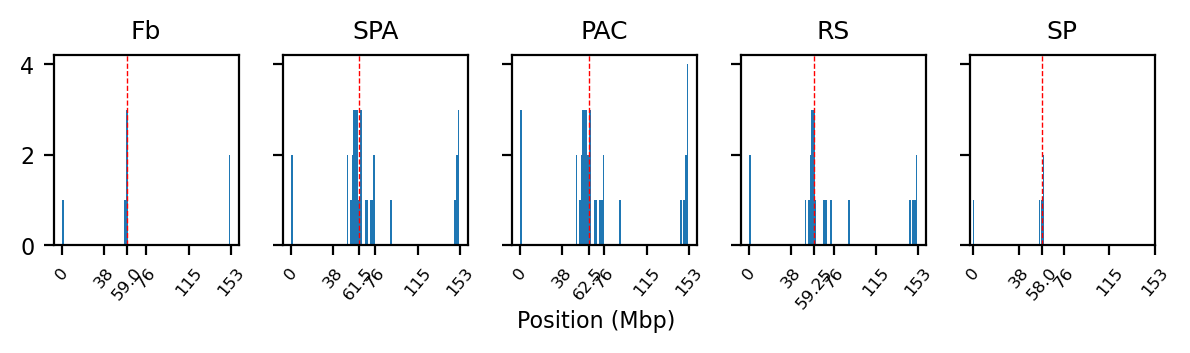
\includegraphics[width=6.19792in,height=1.83333in]{index_files/figure-latex/..-notebooks-05_rec_compartments-fig-e1_nan_hist-output-1.png}

}

\caption{\label{fig-e1_nan_hist}Histogram of NaN values in the E1
eigenvector for each cell type. Median position is marked with a red
dashed line.}

\end{figure}%

The fact that the medians lie within the centromeric region on all cell
sources shows both that the majority of the bad bins are in the
(peri)centromeric region \emph{and} there are approximately equally many
on each side.

\subsection{Compartments (Eigenvectors)}\label{sec-results-eigenvectors}

The three viewframes (\emph{Full}, \emph{Arms}, \emph{10Mb}) for the
calculation of the eigenvectors captured different variability in the
data (Figure~\ref{fig-e1-matrix-full-arms-10mb-round_spermatid}), and as
expected, the inferred compartments (colored red on the E1 tracks) are
more abundant and smaller with smaller viewframes. To determine how well
each of the E1 tracks capture the pattern in the interaction matrix, we
can overlay the matrix with the E1 sign-change and visually determine if
the squares reflect the E1 sign change
(Figure~\ref{fig-e1-matrix-full-arms-10mb-round_spermatid}).

\begin{figure}[H]

\centering{

\centering{

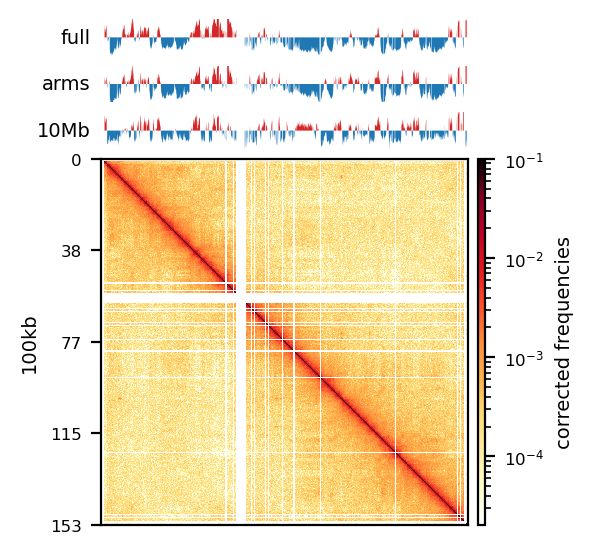
\includegraphics[width=3.09375in,height=2.88542in]{index_files/figure-latex/..-notebooks-07_various_plotting-fig-e1-matrix-full-arms-10mb-round_spermatid-output-1.png}

}

\subcaption{\label{fig-e1-matrix-full-arms-10mb-round_spermatid-1}E1
eigenvector values for merged round spermatid samples at a) 100kb or b)
500kb resolution, as well as the interaction matrix. E1 was restricted
to either Full-chromosome (top), Chromosome-arms (middle), or 10Mb
windows (bottom)}

\centering{

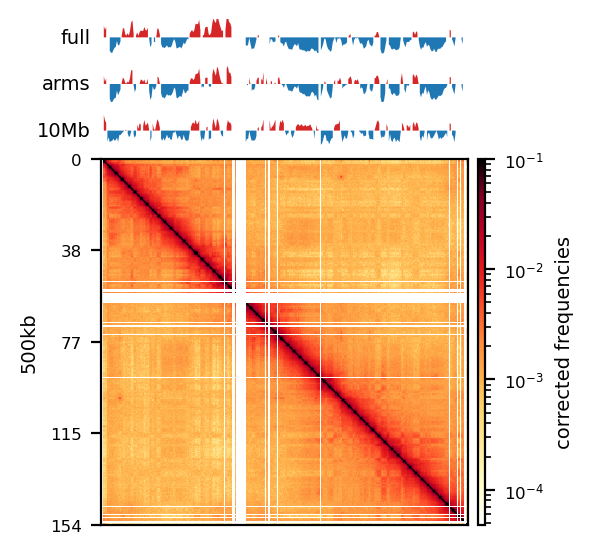
\includegraphics[width=3.09375in,height=2.88542in]{index_files/figure-latex/..-notebooks-07_various_plotting-fig-e1-matrix-full-arms-10mb-round_spermatid-output-2.png}

}

\subcaption{\label{fig-e1-matrix-full-arms-10mb-round_spermatid-2}}

}

\caption{\label{fig-e1-matrix-full-arms-10mb-round_spermatid}}

\end{figure}%

I decide that without more finescaled knowledge than the position of the
centromeres, the arbitrary size of the 10 Mb windowed E1 can not fully
be justified. That is, we could arbitrarily calculate any windowed E1
track. Also, Wang et al. (2019) concludes only for pachytene
spermatocyte to show local interactions in the 10Mb viewframe (what they
refer to as \emph{refined A/B-compartments}), and all the other stages
of spermatogenesis were consistent with the conventional A/B
compartments. The reasonable thing to do is therefore to continue the
analysis, focusing on the arms-restricted eigendecomposition.
Nevertheless, we also keep \emph{refined} compartments in the analysis.

Additionally, as I created coolers with two different sets of parsing
parameters we will compare the resulting matrices and their compartments
(Figure~\ref{fig-rs100-recpe-pe}). As expected, we observe more empty
bins in the Hi-C matrix when comparing the initial run (\texttt{mask})
to the recommended parameters (\texttt{5unique}), but otherwise, the
interaction pattern is indestinguishable. The effect on the E1 is more
noticable, where the absolute magnitude of the E1 values is generally
smaller. There is, however, a small region that changes sign (from A to
B) on the 10Mb-windowed (`refined') E1 track
(Figure~\ref{fig-rs100-recpe-pe};c+d). This region is surrounded by
added empty bins, which could mean that too many low quality pairs in
\texttt{mask} were introducing bias and swapped the sign of E1. It is
supported by the fact that the sign change \emph{only} occured in
\emph{refined} E1, and that the sign after filtering weak pairs
(\(mapq < 30\)) is consistent with the \emph{arms} view. It supports my
previous postulate that it is better to use a viewframe with explicit
molecular meaning than one of an arbitrary window size. That said, the
\texttt{mapq} threshold should really be determined taking both coverage
and resolution into account. For our purposes, and with the \emph{arms}
view, the mapping- and parsing parameters do not seem to be too
sensitive.

\begin{figure}

\begin{minipage}{0.05\linewidth}
~\end{minipage}%
%
\begin{minipage}{0.46\linewidth}

\centering{

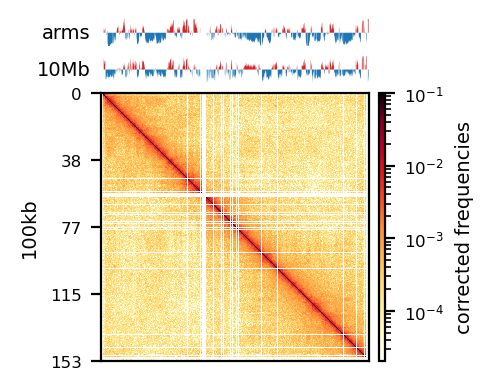
\includegraphics[width=2.57292in,height=2.03125in]{index_files/figure-latex/..-notebooks-07_various_plotting-fig-rs100-recpe-pe-output-1.png}

}

\subcaption{\label{fig-rs100-recpe-pe-1}\texttt{5unique}:
chrX:start-end}

\end{minipage}%
%
\begin{minipage}{0.46\linewidth}

\centering{

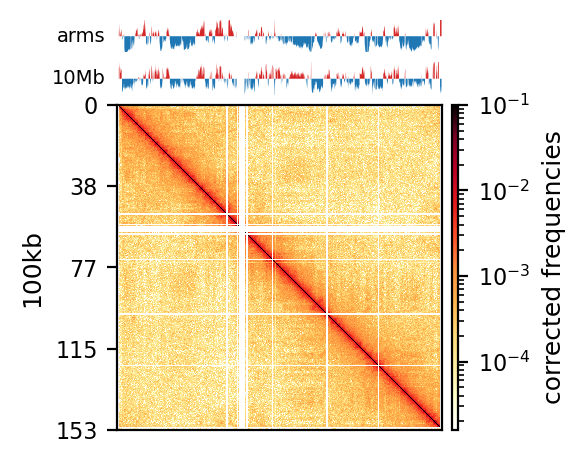
\includegraphics[width=2.57292in,height=2.03125in]{index_files/figure-latex/..-notebooks-07_various_plotting-fig-rs100-recpe-pe-output-2.png}

}

\subcaption{\label{fig-rs100-recpe-pe-2}\texttt{mask}: chrX:start-end}

\end{minipage}%
%
\begin{minipage}{0.05\linewidth}
~\end{minipage}%
\newline
\begin{minipage}{0.05\linewidth}
~\end{minipage}%
%
\begin{minipage}{0.46\linewidth}

\centering{

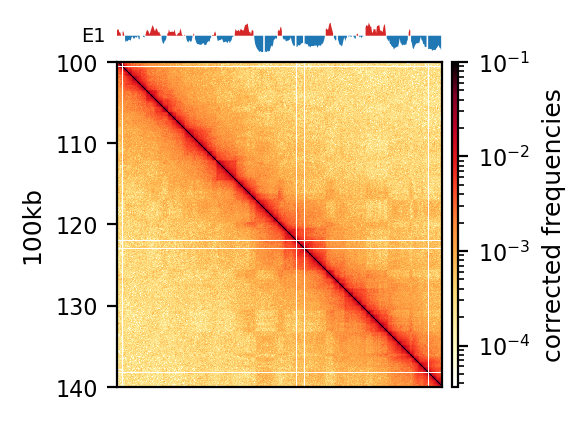
\includegraphics[width=2.57292in,height=2.09375in]{index_files/figure-latex/..-notebooks-07_various_plotting-fig-rs100-recpe-pe-output-3.png}

}

\subcaption{\label{fig-rs100-recpe-pe-3}\texttt{5unique}:
chrX:70Mb-78Mb}

\end{minipage}%
%
\begin{minipage}{0.46\linewidth}

\centering{

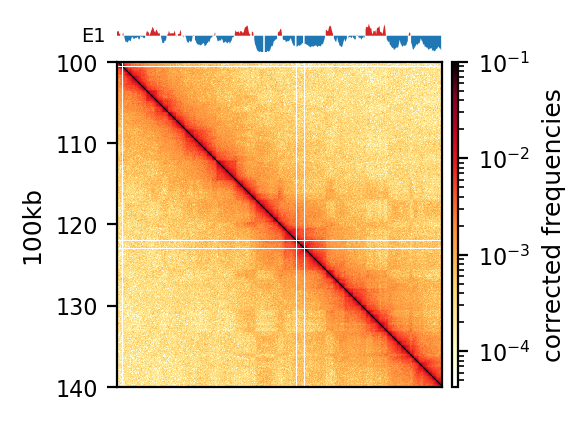
\includegraphics[width=2.57292in,height=2.09375in]{index_files/figure-latex/..-notebooks-07_various_plotting-fig-rs100-recpe-pe-output-4.png}

}

\subcaption{\label{fig-rs100-recpe-pe-4}\texttt{mask}: chrX:70Mb-78Mb}

\end{minipage}%
%
\begin{minipage}{0.05\linewidth}
~\end{minipage}%

\caption{\label{fig-rs100-recpe-pe}Round Spermatid (RS) at 100kb,
comparing the impact of parsing parameters}

\end{figure}%

To emphasize the findings, the sets of A-compartments were compared
between the two parsing runs, showing almost identical compartment
calls. Additionally, the set difference was 8 bins between PE and recPE
for round spermatid 100kb and 5 bins for fibroblast for \emph{arms}
viewframe (Figure~\ref{fig-rs-fb-100-pe-recpe-intervals}; a+b,
respectively). We observe a high number of differences around 76Mb for
the refined compartments (10Mb) of round spermatid, which is consistent
with the sign-flip of E1 values discussed earlier. Anything else would
be surprising, as it is the same data, but visualized in a different
way.

\begin{figure}

\begin{minipage}{0.10\linewidth}
~\end{minipage}%
%
\begin{minipage}{0.40\linewidth}

\centering{

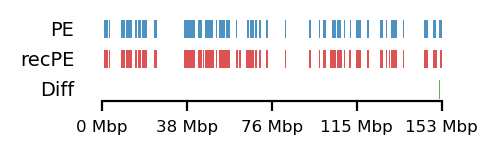
\includegraphics[width=2.59375in,height=0.80208in]{index_files/figure-latex/..-notebooks-07_various_plotting-fig-rs-fb-100-pe-recpe-intervals-output-1.png}

}

\subcaption{\label{fig-rs-fb-100-pe-recpe-intervals-1}RS: arms}

\end{minipage}%
%
\begin{minipage}{0.40\linewidth}

\centering{

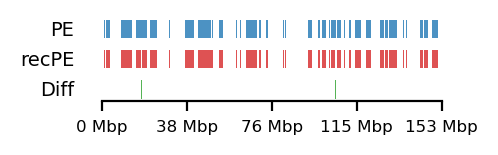
\includegraphics[width=2.59375in,height=0.80208in]{index_files/figure-latex/..-notebooks-07_various_plotting-fig-rs-fb-100-pe-recpe-intervals-output-2.png}

}

\subcaption{\label{fig-rs-fb-100-pe-recpe-intervals-2}Fib: arms}

\end{minipage}%
%
\begin{minipage}{0.10\linewidth}
~\end{minipage}%
\newline
\begin{minipage}{0.10\linewidth}
~\end{minipage}%
%
\begin{minipage}{0.40\linewidth}

\centering{

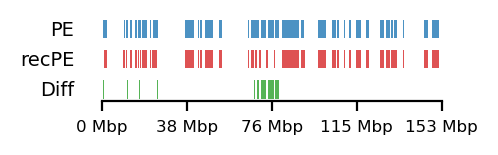
\includegraphics[width=2.59375in,height=0.80208in]{index_files/figure-latex/..-notebooks-07_various_plotting-fig-rs-fb-100-pe-recpe-intervals-output-3.png}

}

\subcaption{\label{fig-rs-fb-100-pe-recpe-intervals-3}RS: 10Mb}

\end{minipage}%
%
\begin{minipage}{0.40\linewidth}

\centering{

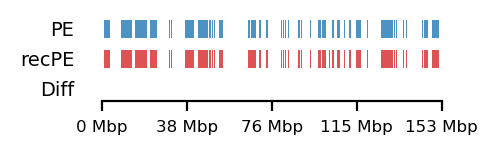
\includegraphics[width=2.59375in,height=0.80208in]{index_files/figure-latex/..-notebooks-07_various_plotting-fig-rs-fb-100-pe-recpe-intervals-output-4.png}

}

\subcaption{\label{fig-rs-fb-100-pe-recpe-intervals-4}Fib: 10Mb}

\end{minipage}%
%
\begin{minipage}{0.10\linewidth}
~\end{minipage}%

\caption{\label{fig-rs-fb-100-pe-recpe-intervals}Round Spermatid (RS)
and Fibroblast (Fb) at 100kb, comparing the impact of parsing parameters
on A-compartment calling at different viewframes; \emph{arms},
\emph{10Mb}. PE: initial parse (masking complex walks); recPE:
recommended parse (reporting the 5'most unique alignment of a complex
walk).}

\end{figure}%

The observed difference between the sets can for our data be attributed
to chance, but we cannot draw general conclusions about the parameters
in general. I argue that the quality and size of the Hi-C library will
influence sensitive to parsing parameters. In that case, the most
flexible approach is still to follow the recommendations from
\texttt{cooler} to report more pairs as valid contacts, and then create
coolers with different \emph{mapq} filters if issues are encountered.

\subsection{Compartment Edges (transition
zones)}\label{compartment-edges-transition-zones}

We compare how the ECH90 regions fit when queried on top of the
A-compartments and equivalently for the edges, for fibroblasts and round
spermatids at 100kb resolution. When queried against the edges in stead,
the the total set size is reduced to less than 50\%. Interestingly, some
of the intersections between A-compartments and ECH90 remain, and new
ones appear as we move to the outside edge of the compartment
(Figure~\ref{fig-comps-edges-ech}). This indicates that most, but not
all, of the intersection between ECH90 regions and the A-compartments
are within 100kb of the compartment edge, and additional overlap is
gained if we define a transition zone on the outside of the edge as
well. To visualize this (outside) edge enrichment, we find the set
difference of the ECH-intersection to compartments and edges,
respectively (Figure~\ref{fig-edge-enrichment}), thus removing all the
`inside' edges. We observe that in almost all of the of the regions of
\(ECH \cap Comp\) are accompanied by an edge also intersecting ECH
(\(ECH \cap Edge\)), localized where the \emph{Diff} track aligns
(within 100kb) with both \(CompInt\) and \(EdgeInt\).

\begin{figure}

\begin{minipage}{0.10\linewidth}
~\end{minipage}%
%
\begin{minipage}{0.40\linewidth}

\centering{

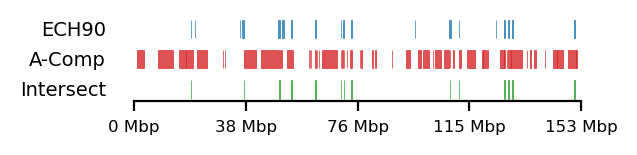
\includegraphics[width=2.58333in,height=0.80208in]{index_files/figure-latex/..-notebooks-07_various_plotting-fig-comps-edges-ech-output-1.png}

}

\subcaption{\label{fig-comps-edges-ech-1}Fibroblast A-compartments}

\end{minipage}%
%
\begin{minipage}{0.40\linewidth}

\centering{

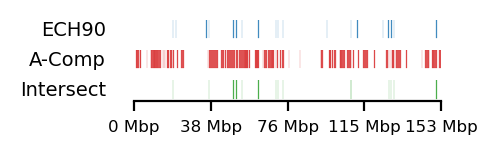
\includegraphics[width=2.58333in,height=0.80208in]{index_files/figure-latex/..-notebooks-07_various_plotting-fig-comps-edges-ech-output-2.png}

}

\subcaption{\label{fig-comps-edges-ech-2}Round Spermatid A-compartments}

\end{minipage}%
%
\begin{minipage}{0.10\linewidth}
~\end{minipage}%
\newline
\begin{minipage}{0.10\linewidth}
~\end{minipage}%
%
\begin{minipage}{0.40\linewidth}

\centering{

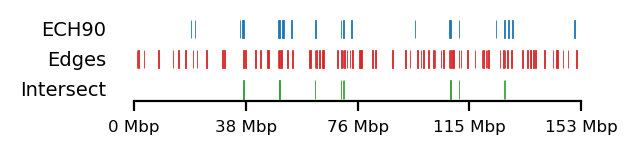
\includegraphics[width=2.58333in,height=0.80208in]{index_files/figure-latex/..-notebooks-07_various_plotting-fig-comps-edges-ech-output-3.png}

}

\subcaption{\label{fig-comps-edges-ech-3}Fibroblast edges}

\end{minipage}%
%
\begin{minipage}{0.40\linewidth}

\centering{

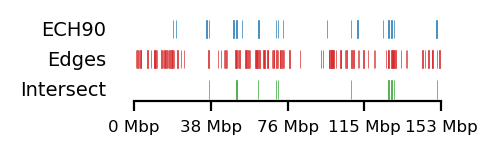
\includegraphics[width=2.58333in,height=0.80208in]{index_files/figure-latex/..-notebooks-07_various_plotting-fig-comps-edges-ech-output-4.png}

}

\subcaption{\label{fig-comps-edges-ech-4}Round Spermatid edges}

\end{minipage}%
%
\begin{minipage}{0.10\linewidth}
~\end{minipage}%

\caption{\label{fig-comps-edges-ech}Visual representation of the genomic
intervals of ECH90, A-compartments (a+b), edges (c+d), and their
intersections. Shown fibroblast (a+c) and round spermatid (b+d) at 100kb
resolution and arms viewframe.}

\end{figure}%

\begin{figure}

\begin{minipage}{0.50\linewidth}

\centering{

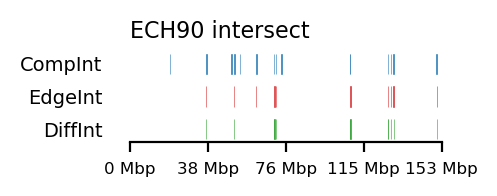
\includegraphics[width=2.58333in,height=1.02083in]{index_files/figure-latex/..-notebooks-07_various_plotting-fig-edge-enrichment-output-1.png}

}

\subcaption{\label{fig-edge-enrichment-1}Round Spermatid}

\end{minipage}%
%
\begin{minipage}{0.50\linewidth}

\centering{

\includegraphics[width=2.58333in,height=1.02083in]{index_files/figure-latex/..-notebooks-07_various_plotting-fig-edge-enrichment-output-2.png}

}

\subcaption{\label{fig-edge-enrichment-2}Fibroblast}

\end{minipage}%

\caption{\label{fig-edge-enrichment}Visual representation of the
enrichment of edges in the intersection of ECH90 and A-compartments.
Shown round spermatid (a) and fibroblast (b) at 100kb resolution and
arms viewframe. Note that the edge-regions are too small to be
distinguished visually from the compartment on the graph, making it look
like they overlap, even though the difference is reported.}

\end{figure}%

We apply both proximity test and Jaccard test, to see how well the
results could occur by chance (Figure~\ref{fig-proximity-jaccard-bar}).
For completeness, the tests are included for all cell types, but we only
use 100kb resolution arms viewframe. We observe that both fibroblast and
round spermatid have \(p < 0.05\) for both tests, meaning the two cell
type have both more intersection with ECH regions than expected by
chance (Jaccard) \emph{and} the non-overlapping intervals are more
proximal to compartment edges than expected by chance (proximity test).
I argue that a significant Jaccard statistic should be interpreted as a
significant amount of overlap between the two sets, i.e.~compartment
edges and ECH90 regions, and the proximity test (when performed on the
edges) gives us information about the potential of expanding or moving
the transition window. That is, if the non-overlapping regions are
\emph{very} proximal, a larger (or shifted) window to only capture the
200kb region outside of the edge might be favourable.

\begin{figure}[H]

\centering{

\includegraphics[width=3.10417in,height=2.05208in]{index_files/figure-latex/..-notebooks-06_rec_genomicintervals-fig-proximity-jaccard-bar-output-1.png}

}

\caption{\label{fig-proximity-jaccard-bar}Proximity and Jaccard index
p-values for ECH90 regions on compartment edges for all cell types at
100kb resolution at arms view \(p=0.05\) is marked as a red line.}

\end{figure}%

\section{Testing against regions of selection in
baboons}\label{testing-against-regions-of-selection-in-baboons}

The data for this analysis was provided by Kasper Munch in bed-like
format, mapped to \emph{panu\_3.0} (PapAnu4) assembly. The intervals
define genomic regions in a hybrid/migrating population of baboon where
strong negative selection acts against minor parent ancestry (Sørensen
et al. 2023). The segments had to be lifted to rheMac10 to be able to
correlate the two sets of intervals. The original UCSC liftOver
(Hinrichs 2006) is very strict and does not try to conserve segments in
favor of accuracy e.g.~inversions or small indels, which results in
highly scattered regions when lifted. To favor preservation of segments,
we use \emph{segment\_liftover} (Gao, Huang, and Baudis 2018), resulting
in much more similar regions to the original
(Figure~\ref{fig-compare-liftover}). As no chain file from
\emph{panu\_3.0} to \emph{Mmul\_10} was available, we had to use
\emph{panu\_2.0} as intermediate.

\begin{figure}[H]

\centering{

\centering{

\includegraphics[width=5.19792in,height=0.80208in]{index_files/figure-latex/..-notebooks-07_various_plotting-fig-compare-liftover-output-1.png}

}

\subcaption{\label{fig-compare-liftover-1}high-olive}

\centering{

\includegraphics[width=5.19792in,height=0.80208in]{index_files/figure-latex/..-notebooks-07_various_plotting-fig-compare-liftover-output-2.png}

}

\subcaption{\label{fig-compare-liftover-2}high-hama}

}

\caption{\label{fig-compare-liftover}Comparison of a) high-olive and b)
high-hama intervals between Panu\_3.0, segment\_liftover, or UCSC
liftOver coordinates.}

\end{figure}%

Initially, the compartment edges of round spermatid at 100kb resolution
(RS100) were plotted against the lifted coordinates from a \emph{P.}
anubis-hamadryas hybrid population, where either all the sampled
individuals have \emph{Papio anubis} ancestry or 95\% of the sampled
individuals have \emph{Papio hamadryas} ancestry. Their respective
intersections were plotted undeneath. We expect less intersection for
\emph{hamadryas} than for \emph{anubis} as the total set size is much
smaller. The compartment edges and \emph{Papio anubis}-derived
regions(Figure~\ref{fig-baboon-rs100-intersect}; b) seem to be highly
enriched in the first 25 Mbp, and thus it has a high degree of
intersection with the compartment edges. Interestingly, the ECH90 set is
nearly empty in that region, making the finding outside the scope of
this analysis, although it could be useful for determining the mechanism
for selecting the \emph{P.anubis} ancestral allele in the hybrid baboon
population. The \emph{P.hamadryas}-derived regions seem intersect the
compartment edges more centered on the chromosome
(Figure~\ref{fig-baboon-rs100-intersect}; a). The proximity test ruled
out that the non-intersecting parts of the respective regions were this
proximal by chance. However, the Jaccard test revealed that the
intersection between the RS100 and both Hi-\emph{P.hama} and
Hi-\emph{P.anu} can be explained by chance alone .

\begin{figure}

\begin{minipage}{0.10\linewidth}
~\end{minipage}%
%
\begin{minipage}{0.40\linewidth}

\centering{

\includegraphics[width=2.58333in,height=0.80208in]{index_files/figure-latex/..-notebooks-07_various_plotting-fig-baboon-rs100-intersect-output-1.png}

}

\subcaption{\label{fig-baboon-rs100-intersect-1}\emph{P. hamadryas} +
arms E1}

\end{minipage}%
%
\begin{minipage}{0.40\linewidth}

\centering{

\includegraphics[width=2.58333in,height=0.80208in]{index_files/figure-latex/..-notebooks-07_various_plotting-fig-baboon-rs100-intersect-output-2.png}

}

\subcaption{\label{fig-baboon-rs100-intersect-2}\emph{P. anubis} + arms
E1}

\end{minipage}%
%
\begin{minipage}{0.10\linewidth}
~\end{minipage}%
\newline
\begin{minipage}{0.10\linewidth}
~\end{minipage}%
%
\begin{minipage}{0.40\linewidth}

\centering{

\includegraphics[width=2.58333in,height=0.80208in]{index_files/figure-latex/..-notebooks-07_various_plotting-fig-baboon-rs100-intersect-output-3.png}

}

\subcaption{\label{fig-baboon-rs100-intersect-3}\emph{P. hamadryas} +
10Mb E1}

\end{minipage}%
%
\begin{minipage}{0.40\linewidth}

\centering{

\includegraphics[width=2.58333in,height=0.80208in]{index_files/figure-latex/..-notebooks-07_various_plotting-fig-baboon-rs100-intersect-output-4.png}

}

\subcaption{\label{fig-baboon-rs100-intersect-4}\emph{P. anubis} + 10Mb
E1}

\end{minipage}%
%
\begin{minipage}{0.10\linewidth}
~\end{minipage}%

\caption{\label{fig-baboon-rs100-intersect}Comparing the A-compartments
of round spermatid (RS) with regions in baboons from hybrid population
where a) 95\% of sampled individuals have \emph{Papio hamadryas}
ancestry or b) 100\% of the samples have \emph{Papio anubis} ancestry.
The regions are extracted and lifted from panu4.0 reference to rhemac10,
then collapsed to non-overlapping intervals with \texttt{genominterv}.}

\end{figure}%

\newpage{}

\chapter{Discussion}\label{discussion}

Here is the discussion

\chapter*{Bibliography}\label{bibliography}
\addcontentsline{toc}{chapter}{Bibliography}

\begingroup
\raggedright

\phantomsection\label{refs}
\begin{CSLReferences}{1}{0}
\bibitem[\citeproctext]{ref-abdennur2020coolerscalablestorage}
Abdennur, Nezar, and Leonid A Mirny. 2020. {``Cooler: Scalable Storage
for {Hi-C} Data and Other Genomically Labeled Arrays.''} Edited by
Jonathan Wren. \emph{Bioinformatics} 36 (1): 311--16.
\url{https://doi.org/10.1093/bioinformatics/btz540}.

\bibitem[\citeproctext]{ref-bicciato2022hicdataanalysis}
Bicciato, Silvio, and Francesco Ferrari, eds. 2022. \emph{Hi-{C Data
Analysis}: {Methods} and {Protocols}}. Vol. 2301. Methods in {Molecular
Biology}. New York, NY: Springer US.
\url{https://doi.org/10.1007/978-1-0716-1390-0}.

\bibitem[\citeproctext]{ref-bravonunez2018geneticvillainskiller}
Bravo Núñez, María Angélica, Nicole L. Nuckolls, and Sarah E. Zanders.
2018. {``Genetic {Villains}: {Killer Meiotic Drivers}.''} \emph{Trends
in Genetics} 34 (6): 424--33.
\url{https://doi.org/10.1016/j.tig.2018.02.003}.

\bibitem[\citeproctext]{ref-devteam2024sratoolkit}
DevTeam, SRA Toolkit. 2024. {``{SRA Toolkit}.''} Wiki. \emph{GitHub}.
https://github.com/ncbi/sra-tools/wiki/01.-Downloading-SRA-Toolkit.
\url{https://trace.ncbi.nlm.nih.gov/Traces/sra/sra.cgi?view=software}.

\bibitem[\citeproctext]{ref-ewels2016multiqcsummarizeanalysis}
Ewels, Philip, Måns Magnusson, Sverker Lundin, and Max Käller. 2016.
{``{MultiQC}: Summarize Analysis Results for Multiple Tools and Samples
in a Single Report.''} \emph{Bioinformatics} 32 (19): 3047--48.
\url{https://doi.org/10.1093/bioinformatics/btw354}.

\bibitem[\citeproctext]{ref-gao2018segment_liftoverpythontool}
Gao, Bo, Qingyao Huang, and Michael Baudis. 2018. {``Segment\_liftover :
A {Python} Tool to Convert Segments Between Genome Assemblies.''}
\emph{F1000Research} 7 (June): 319.
\url{https://doi.org/10.12688/f1000research.14148.2}.

\bibitem[\citeproctext]{ref-hinrichs2006ucscgenomebrowser}
Hinrichs, A. S. 2006. {``The {UCSC Genome Browser Database}: Update
2006.''} \emph{Nucleic Acids Research} 34 (90001): D590--98.
\url{https://doi.org/10.1093/nar/gkj144}.

\bibitem[\citeproctext]{ref-imakaev2012iterativecorrectionhic}
Imakaev, Maxim, Geoffrey Fudenberg, Rachel Patton McCord, Natalia
Naumova, Anton Goloborodko, Bryan R Lajoie, Job Dekker, and Leonid A
Mirny. 2012. {``Iterative Correction of {Hi-C} Data Reveals Hallmarks of
Chromosome Organization.''} \emph{Nature Methods} 9 (10): 999--1003.
\url{https://doi.org/10.1038/nmeth.2148}.

\bibitem[\citeproctext]{ref-jaenike2001sexchromosomemeiotic}
Jaenike, John. 2001. {``Sex {Chromosome Meiotic Drive}.''} \emph{Annual
Review of Ecology and Systematics} 32 (1): 25--49.
\url{https://doi.org/10.1146/annurev.ecolsys.32.081501.113958}.

\bibitem[\citeproctext]{ref-lajoie2015hitchhikersguidehic}
Lajoie, Bryan R., Job Dekker, and Noam Kaplan. 2015. {``The
{Hitchhiker}'s {Guide} to {Hi-C Analysis}: {Practical} Guidelines.''}
\emph{Methods (San Diego, Calif.)} 72 (January): 65--75.
\url{https://doi.org/10.1016/j.ymeth.2014.10.031}.

\bibitem[\citeproctext]{ref-lieberman-aiden2009comprehensivemappinglongrange}
Lieberman-Aiden, Erez, Nynke L. Van Berkum, Louise Williams, Maxim
Imakaev, Tobias Ragoczy, Agnes Telling, Ido Amit, et al. 2009.
{``Comprehensive {Mapping} of {Long-Range Interactions Reveals Folding
Principles} of the {Human Genome}.''} \emph{Science} 326 (5950):
289--93. \url{https://doi.org/10.1126/science.1181369}.

\bibitem[\citeproctext]{ref-munch2024munchgroup}
Munch, Kasper. 2024. {``Munch-Group.''}
https://munch-group.org/research.html.

\bibitem[\citeproctext]{ref-openchromosomecollective}
{``Open {Chromosome Collective} ({Open2C}).''} n.d. Resource.
\emph{Open2C}. https://open2c.github.io/. Accessed November 13, 2024.

\bibitem[\citeproctext]{ref-open2c2024pairtoolssequencingdata}
Open2C, Nezar Abdennur, Geoffrey Fudenberg, Ilya M. Flyamer, Aleksandra
A. Galitsyna, Anton Goloborodko, Maxim Imakaev, and Sergey V. Venev.
2024. {``Pairtools: {From} Sequencing Data to Chromosome Contacts.''}
Edited by Ferhat Ay. \emph{PLOS Computational Biology} 20 (5): e1012164.
\url{https://doi.org/10.1371/journal.pcbi.1012164}.

\bibitem[\citeproctext]{ref-skov2023extraordinaryselectionhuman}
Skov, Laurits, Moisès Coll Macià, Elise Anne Lucotte, Maria Izabel Alves
Cavassim, David Castellano, Mikkel Heide Schierup, and Kasper Munch.
2023. {``Extraordinary Selection on the Human {X} Chromosome Associated
with Archaic Admixture.''} \emph{Cell Genomics} 3 (3): 100274.
\url{https://doi.org/10.1016/j.xgen.2023.100274}.

\bibitem[\citeproctext]{ref-sorensen2023genomewidecoancestryreveals}
Sørensen, Erik F., R. Alan Harris, Liye Zhang, Muthuswamy Raveendran,
Lukas F. K. Kuderna, Jerilyn A. Walker, Jessica M. Storer, et al. 2023.
{``Genome-Wide Coancestry Reveals Details of Ancient and Recent
Male-Driven Reticulation in Baboons.''} \emph{Science} 380 (6648):
eabn8153. \url{https://doi.org/10.1126/science.abn8153}.

\bibitem[\citeproctext]{ref-wang2019reprogrammingmeioticchromatin}
Wang, Yao, Hanben Wang, Yu Zhang, Zhenhai Du, Wei Si, Suixing Fan,
Dongdong Qin, et al. 2019. {``Reprogramming of {Meiotic Chromatin
Architecture} During {Spermatogenesis}.''} \emph{Molecular Cell} 73 (3):
547--561.e6. \url{https://doi.org/10.1016/j.molcel.2018.11.019}.

\bibitem[\citeproctext]{ref-warren2020sequencediversityanalyses}
Warren, Wesley C., R. Alan Harris, Marina Haukness, Ian T. Fiddes,
Shwetha C. Murali, Jason Fernandes, Philip C. Dishuck, et al. 2020.
{``Sequence Diversity Analyses of an Improved Rhesus Macaque Genome
Enhance Its Biomedical Utility.''} \emph{Science} 370 (6523): eabc6617.
\url{https://doi.org/10.1126/science.abc6617}.

\end{CSLReferences}

\endgroup


\backmatter


\end{document}
